\documentclass[a4paper, 12pt]{book}
% \newcommand{\abs}[1]{\lvert #1 \rvert}
\usepackage{course}
\newcommand{\one}{\text{\usefont{U}{bbold}{m}{n}1}}

%--- Fixed head height to satisfy scrlayer-scrpage's minimum.
\setlength{\headheight}{15pt}

%--- The documentation for the title can be found at: https://en.wikibooks.org/wiki/LaTeX/Title_Creation
\title{Machine (or Automated) Learning}
\subtitle{Lecture Notes with Python Companions}
\author{Ahmed U. Ashraf}
\date{\today}

\begin{document}

\frontmatter
\maketitle
%--- Make every table-of-contents item a hyperlink target, so that the
%--- chapter/section headings can link back to their ToC entry.
\makeatletter
\let\hypercontentsline=\contentsline
\renewcommand{\contentsline}[4]{%
  \hypertarget{toc.#4}{}\hypercontentsline{#1}{#2}{#3}{#4}}
\makeatother
%--- We print ToC: Table of Contents
\tableofcontents\label{toc}

\chapter*{Preface}
\addcontentsline{toc}{chapter}{Preface}

These notes collect the core ideas of a first course in machine learning. They are
organised around three questions: \emph{what} are we trying to learn, \emph{how} do
we learn it from data, and \emph{how do we know} that what we learned will work on
new observations? The mathematical prerequisites are reviewed in
Chapters~\ref{ch:calc} and~\ref{ch:prob}; no prior machine-learning background is
assumed.

Each methodological chapter ends with a \emph{code companion}: a short, runnable
Python script in the \texttt{Code/} folder that reproduces the main ideas with
\texttt{scikit-learn}, \texttt{NumPy}, and \texttt{matplotlib}. The scripts are
deliberately small and self-contained; they are meant to be read, modified, and
broken. Jupyter notebooks in the same folder expand on the mathematical background,
the distance metrics, probability, and the worked machine-learning examples.

\begin{quote}
\emph{All models are wrong, but some are useful.} --- George E. P. Box
\end{quote}

\section*{Notation}
\addcontentsline{toc}{section}{Notation}

\begin{center}
\renewcommand{\arraystretch}{1.25}
\begin{tabular}{ll}
\toprule
Symbol & Meaning \\
\midrule
$\mathbf{x} \in \R^d$ & input (feature) vector \\
$y$ or $t$ & target (label, response) \\
$n$ & number of training examples \\
$d$ or $p$ & number of features \\
$\mathbf{X} \in \R^{n \times d}$ & design matrix, one example per row \\
$\boldsymbol{\beta}$ & model parameters \\
$\hat{y}$ & prediction \\
$\ell(\cdot,\cdot)$ & loss function \\
$\mathscr{D}$ & data distribution \\
$\mathcal{H}$ & hypothesis class \\
$\risk(\cdot)$ & risk (expected loss) \\
$\norm{\cdot}_1, \norm{\cdot}_2$ & $\ell_1$ and $\ell_2$ norms \\
$\nabla f$, $H_f$ & gradient and Hessian of $f$ \\
$\E[\cdot]$, $\Var[\cdot]$ & expectation and variance \\
$\mathscr{N}(\mu,\Sigma)$ & Gaussian distribution \\
\bottomrule
\end{tabular}
\end{center}

\newpage
\section*{Abbreviations}
\addcontentsline{toc}{section}{Abbreviations}

\begin{center}
\renewcommand{\arraystretch}{1.25}
\begin{tabular}{ll}
\toprule
Abbreviation & Meaning \\
\midrule
CDF & Cumulative Distribution Function \\
CNN & Convolutional Neural Network \\
PCA & Principal Component Analysis \\
PDF & Probability Density Function \\
PGM & Probabilistic Graphic Models \\  
PSD & positive semidefinite \\
SAD & Sum of Absolute Differences \\
SVM & Support Vector Machines \\
TV & Total Variation \\
\bottomrule
\end{tabular}
\end{center}

\newpage
\section*{Common Datasets}
\addcontentsline{toc}{section}{Common Datasets}

\begin{center}
\renewcommand{\arraystretch}{1.25}
\begin{tabular}{ll}
\toprule
Dataset & Details \\
\midrule
Iris & 150 flowers, 3 species, 4 numeric features; a small multiclass baseline. \\
Digits & 1,797 images of $8\times8$ pixels; a fast stand-in for MNIST. \\
MNIST & 70,000 handwritten digits ($28\times28$ pixels), split 60k/10k. \\
Breast cancer & 569 diagnostic measurements, 2 classes; a binary benchmark. \\
Two moons & Synthetic interleaving crescents needing a non-linear boundary. \\
\bottomrule
\end{tabular}
\end{center}

\mainmatter

\chapter{Mathematical Background}
\label{ch:calc}

\section{Linear algebra}

\subsection{Vectors, matrices, and norms}

We write vectors as columns and use
\begin{align}
    \mathbf{x}^\top \mathbf{y} = \sum_{i=1}^d x_i y_i
\end{align}
for the Euclidean inner product. The most common norms are
\begin{align}
    \norm{\mathbf{x}}_1 &\defn \sum_{i=1}^d |x_i|, \\
    \norm{\mathbf{x}}_2 &\defn \sqrt{\sum_{i=1}^d x_i^2}, \\
    \norm{\mathbf{x}}_\infty &\defn \max_i |x_i|.
\end{align}
\begin{example}[Norms of a vector]
    For $\mathbf{x} = (3,-4)^\top$,
    \begin{align}
        \norm{\mathbf{x}}_1 &= |3|+|-4| = 7, &
        \norm{\mathbf{x}}_2 &= \sqrt{3^2+(-4)^2} = 5, \\
        \norm{\mathbf{x}}_\infty &= \max\{3,4\} = 4.
    \end{align}
    The $\ell_2$ norm is the ordinary Euclidean length, while the $\ell_1$ norm is
    the sum of absolute coordinates and often encourages sparsity when used as a
    penalty.
\end{example}

\begin{definition}
    A symmetric matrix ${A}$ is \emph{positive semidefinite}\index{positive semidefinite} (PSD)\index{PSD} if
    \begin{align}
        \mathbf{x}^\top {A}\mathbf{x} \geq 0
    \end{align}
    for all $\mathbf{x}$. We call it \emph{positive definite}\index{positive definite} if the inequality is strict for $\mathbf{x} \neq \mathbf{0}$.
\end{definition}

\begin{example}[Positive definite, semidefinite, and indefinite matrices]
    The matrix
    \begin{align}
        {A} &= \begin{bmatrix}2&1\\1&2\end{bmatrix}
    \end{align}
    has eigenvalues $1$ and $3$, so it is positive definite. The matrix
    \begin{align}
        {B} &= \begin{bmatrix}1&1\\1&1\end{bmatrix}
    \end{align}
    has eigenvalues $0$ and $2$: it is PSD but not positive definite, because
    $\mathbf{v}=(1,-1)^\top$ gives $\mathbf{v}^\top{B}\mathbf{v}=0$. The matrix
    \begin{align}
        C &= \begin{bmatrix}1&2\\2&1\end{bmatrix}    
    \end{align}
    has an eigenvalue $-1$, so it
    is neither PSD nor positive definite.
\end{example}

\begin{example}[Gram matrices are PSD]
    For any real matrix $X \in \R^{n \times d}$, the Gram matrix
    $X^\top X$ is PSD because
    \begin{align}
        \mathbf{v}^\top X^\top X\mathbf{v}
        = (\norm{X\mathbf{v}}_2)^2 \geq 0.
    \end{align}
    It is positive definite exactly when $X$ has full column rank: if
    $X\mathbf{v}=\mathbf{0}$ for some $\mathbf{v}\neq\mathbf{0}$, then the
    quadratic form vanishes.
\end{example}

\begin{theorem}
    Every covariance matrix is positive semidefinite.
\end{theorem}
\begin{proof}
    Let $X$ be a random vector with mean $\mu$. Its covariance
    matrix is
    \begin{align}
        \Sigma
        = \E\big[(X-\mu)(X-\mu)^\top\big].
    \end{align}
    For any vector $\mathbf{a}$,
    \begin{align}
        \mathbf{a}^\top\Sigma\mathbf{a} &= \E\big[\mathbf{a}^\top(X-\mu)
          (X-\mu)^\top\mathbf{a}\big]\\
       & = \E\big[(\mathbf{a}^\top(X-\mu))^2\big] \geq 0.
    \end{align}
    Hence $\Sigma$ is PSD. It is positive definite unless some non-zero
    linear combination of the coordinates of $X$ is almost surely constant.
\end{proof}

\begin{example}[Covariance matrices for two features]
    Suppose two features have variances $1$ and $4$ and covariance $1$. Their
    covariance matrix is
    \begin{align}
        {\Sigma} = \begin{bmatrix}1&1\\1&4\end{bmatrix}.
    \end{align}
    Its determinant is $1\cdot4-1\cdot1=3>0$ and its trace is $5>0$, so both
    eigenvalues are positive and ${\Sigma}$ is positive definite.
\end{example}

\begin{example}[A rank-one covariance matrix]
    If two features are perfectly correlated, for example $X_2 = 2X_1$ with
    $\Var(X_1)=1$, then
    \begin{align}
        {\Sigma}
        = \begin{bmatrix}1&2\\2&4\end{bmatrix}
        = \begin{bmatrix}1\\2\end{bmatrix}\begin{bmatrix}1&2\end{bmatrix}.
    \end{align}
    This matrix has eigenvalues $0$ and $5$: it is PSD but not positive definite. The
    zero eigenvalue corresponds to the direction $(2,-1)^\top$, along which the data
    have no variation.
\end{example}

\begin{theorem}
    If $\mathbf{x}^\star$ is a local minimizer of a twice continuously differentiable
    function $f$, then the Hessian $H_f(\mathbf{x}^\star)$ is positive semidefinite.
\end{theorem}
\begin{proof}
    Let $\mathbf{u}$ be any direction and define the one-dimensional function
    $g(t) = f(\mathbf{x}^\star + t\mathbf{u})$. Since $\mathbf{x}^\star$ is a local
    minimizer of $f$, $t=0$ is a local minimizer of $g$. Therefore
    $g'(0)=0$ and $g''(0)\geq 0$. By the chain rule,
    \begin{align}
        g'(t) = \nabla f(\mathbf{x}^\star+t\mathbf{u})^\top\mathbf{u},
        \qquad
        g''(t) = \mathbf{u}^\top H_f(\mathbf{x}^\star+t\mathbf{u})\,\mathbf{u}.
    \end{align}
    At $t=0$, $g''(0)=\mathbf{u}^\top H_f(\mathbf{x}^\star)\mathbf{u}\geq 0$. Since
    $\mathbf{u}$ was arbitrary, $H_f(\mathbf{x}^\star)$ is PSD.
\end{proof}

\begin{example}[One-dimensional minima and inflection points]
    For $f(x)=x^2$ at $x=0$, $f'(0)=0$ and $f''(0)=2>0$, so the Hessian is positive
    definite and the point is a strict local minimum. For $f(x)=x^4$ at $x=0$,
    $f'(0)=0$ and $f''(0)=0$: the Hessian is only PSD, yet the point is still a local
    minimum. For $f(x)=x^3$ at $x=0$, again $f'(0)=0$ and $f''(0)=0$, but the point is
    not a minimum. This shows that a PSD Hessian at a stationary point is necessary,
    not sufficient, for a local minimum.
\end{example}

\begin{example}[A saddle point in two dimensions]
    For $f(x,y)=x^2-y^2$ at $(0,0)$, the gradient is zero and the Hessian is
    \begin{align}
        H_f(0,0) = \begin{bmatrix}2&0\\0&-2\end{bmatrix},
    \end{align}
    which is indefinite. The point is a saddle, not a minimum. By contrast,
    $f(x,y)=x^2+y^2$ has Hessian $2\mathbf{1}$ at the origin, which is positive
    definite, and the origin is a strict local (and global) minimum.
\end{example}

\subsection{Useful matrix identities}

For invertible matrices and vectors of compatible dimensions,
\begin{align}
    \nabla_{\mathbf{x}} (\mathbf{a}^\top \mathbf{x}) &= \mathbf{a}, &
    \nabla_{\mathbf{x}} (\mathbf{x}^\top \mathbf{A}\mathbf{x}) &= (A+A^\top)\mathbf{x},\\
    \nabla_{\mathbf{X}} \norm{\mathbf{X}}_F^2 &= 2\mathbf{X}, &
    \nabla_{\mathbf{X}} \tr(\mathbf{A}\mathbf{X}) &= \mathbf{A}^\top.
\end{align}
If $\mathbf{A}$ is symmetric, $\nabla_{\mathbf{x}} \mathbf{x}^\top \mathbf{A}\mathbf{x}
= 2\mathbf{A}\mathbf{x}$.

\section{Calculus}

Differentiation is the operation of transforming one mathematical function to another, called the derivative. The derivative tells the slope, or the rate of change, of the original function.

\subsection{Gradients}

\begin{definition}
    The \emph{gradient} of a differentiable function $f : \R^d \to \R$ at a point $\mathbf{x}$ is the vector of partial derivatives
    \begin{align}
    \nabla f(\mathbf{x}) =
    \begin{bmatrix}
        \dfrac{\partial f}{\partial x_1}(\mathbf{x})\\
        \vdots\\
        \dfrac{\partial f}{\partial x_d}(\mathbf{x})
    \end{bmatrix}.
    \end{align}
    The gradient points in the direction of steepest ascent.
\end{definition}

\begin{example}[Gradient of a polynomial]
    For $f(x,y)=x^2y+3y$,
    \begin{align}
        \nabla f(x,y) = \begin{bmatrix}2xy\\ x^2+3\end{bmatrix}.
    \end{align}
    At $(1,2)$ the gradient is $(4,4)^\top$, so moving in the direction $(1,1)^\top$
    increases $f$ most rapidly at that point.
\end{example}

\begin{example}[Gradient of a least-squares objective]
    For $f(\mathbf{x})=\frac12\norm{\mathbf{A}\mathbf{x}-\mathbf{b}}_2^2$,
    \begin{align}
        \nabla f(\mathbf{x})
        = \mathbf{A}^\top(\mathbf{A}\mathbf{x}-\mathbf{b}).
    \end{align}
    Setting the gradient to zero recovers the normal equations
    $\mathbf{A}^\top\mathbf{A}\mathbf{x}=\mathbf{A}^\top\mathbf{b}$.
\end{example}

\subsection{Directional derivative}
\begin{definition}
    The \emph{directional derivative} of $f$ at a point $\mathbf{x}$ in the direction $\mathbf{u}$ (with $\norm{\mathbf{u}}=1$) is
    \begin{align}
    D_{\mathbf{u}} f(\mathbf{x}) &\defn \nabla f(\mathbf{x})^\top \mathbf{u}
    = \sum_{i=1}^{d} \frac{\partial f}{\partial x_i}(\mathbf{x}) u_i.
    \end{align}
    Its value at $\mathbf{x}_0$ is given by
    \begin{align}
          (D_{\mathbf{u}} f)(\mathbf{x}_0)
          &= \lim_{h \to 0} \frac{f(\mathbf{x}_0 + h\mathbf{u}) - f(\mathbf{x}_0)}{h}.
    \end{align}
\end{definition}
Consequently, $-\nabla f(\mathbf{x})$ is the direction of steepest descent, which is
the intuition behind gradient-based optimisation.

\begin{example}[Directional derivative]
    Let $f(x,y)=x^2+y^2$ and $\mathbf{u}=(3/5,4/5)^\top$, which is a unit vector.
    At $(1,2)$,
    \begin{align}
        \nabla f(1,2) = (2,4)^\top,
        \qquad
        D_{\mathbf{u}}f(1,2) = 2\cdot\frac35 + 4\cdot\frac45 = \frac{22}{5}.
    \end{align}
    Moving a small distance $h$ in direction $\mathbf{u}$ therefore changes $f$ by
    approximately $\frac{22}{5}h$.
\end{example}

\begin{example}[Steepest ascent]
    For the same function, the unit direction of steepest ascent at $(1,2)$ is
    \begin{align}
        \mathbf{u}^\star = \frac{\nabla f(1,2)}{\norm{\nabla f(1,2)}_2}
        = \frac{1}{\sqrt{20}}(2,4)^\top = \frac{1}{\sqrt5}(1,2)^\top.
    \end{align}
    The directional derivative in this direction is
    $\norm{\nabla f(1,2)}_2=\sqrt{20}$, which is the largest value of
    $D_{\mathbf{u}}f(1,2)$ over all unit vectors $\mathbf{u}$ by the
    Cauchy--Schwarz inequality.
\end{example}

\subsection{Jacobian}

If $\mathbf{g} : \R^n \to \R^m$ is differentiable, its \emph{Jacobian}\index{Jacobian} is the $m \times n$ matrix $J_{\mathbf{g}}(\mathbf{x})$ with entries
\begin{align}
    (J_{\mathbf{g}})_{ij} = \frac{\partial g_i}{\partial x_j}.
\end{align}
\begin{example}[Jacobian of a vector-valued function]
    Define the map
    \begin{align}
        \mathbf{g}(x,y) = (x^2y,\ \sin x,\ x+y).
    \end{align}
    Its Jacobian is
    \begin{align}
        J_{\mathbf{g}}(x,y) =
        \begin{bmatrix}
            2xy & x^2\\
            \cos x & 0\\
            1 & 1
        \end{bmatrix}.
    \end{align}
    The first row is the gradient of the first component, the second row is the
    gradient of the second component, and so on.
\end{example}

\begin{example}[Jacobian of polar coordinates]
    The map from polar to Cartesian coordinates is
    \begin{align}
        \mathbf{g}(r,\theta) = (r\cos\theta,\ r\sin\theta),
    \end{align}
    with Jacobian
    \begin{align}
        J_{\mathbf{g}}(r,\theta) =
        \begin{bmatrix}
            \cos\theta & -r\sin\theta\\
            \sin\theta & r\cos\theta
        \end{bmatrix}.
    \end{align}
    Its determinant is $r$, which is the area-scaling factor used when changing from
    Cartesian to polar coordinates in integrals.
\end{example}

\subsection{Chain rule}
\begin{proposition}\label{prop:nabla-jacob}
    For $h(\mathbf{x}) = f(\mathbf{g}(\mathbf{x}))$ with $f : \R^m \to \R$,
\begin{align}
    \nabla h(\mathbf{x}) = J_{\mathbf{g}}(\mathbf{x})^\top \nabla f(\mathbf{g}(\mathbf{x})).
\end{align}
\end{proposition}
\begin{proof}
    Write $\mathbf{y}=\mathbf{g}(\mathbf{x})$ and $y_i=g_i(\mathbf{x})$. By the
    multivariate chain rule,
    \begin{align}
        \frac{\partial h}{\partial x_j}(\mathbf{x})
        = \sum_{i=1}^m
          \frac{\partial f}{\partial y_i}(\mathbf{g}(\mathbf{x}))
          \frac{\partial g_i}{\partial x_j}(\mathbf{x})
        = \sum_{i=1}^m
          (J_{\mathbf{g}})_{ij}(\mathbf{x})\,
          \frac{\partial f}{\partial y_i}(\mathbf{g}(\mathbf{x})).
    \end{align}
    The final expression is exactly the $j$-th entry of
    $J_{\mathbf{g}}(\mathbf{x})^\top\nabla f(\mathbf{g}(\mathbf{x}))$.
\end{proof}
This proposition \ref{prop:nabla-jacob} is the engine behind backpropagation in neural networks
(Chapter~\ref{ch:nn}).
\begin{example}[Chain rule with a linear map]
    Let $f(u,v)=u^2+v^2$ and $\mathbf{g}(x,y)=(x+y,\ x-y)$. Then
    \begin{align}
        h(x,y) = f(\mathbf{g}(x,y)) = (x+y)^2+(x-y)^2 = 2x^2+2y^2,
    \end{align}
    so $\nabla h(x,y)=(4x,4y)^\top$. Checking the proposition,
    \begin{align}
        J_{\mathbf{g}} = \begin{bmatrix}1&1\\1&-1\end{bmatrix},
        \qquad
        \nabla f(\mathbf{g}(x,y)) = \begin{bmatrix}2(x+y)\\2(x-y)\end{bmatrix},
        \qquad
        J_{\mathbf{g}}^\top\nabla f = \begin{bmatrix}4x\\4y\end{bmatrix}.
    \end{align}
\end{example}

\subsection{Hessian}

\begin{definition}
    The \emph{Hessian}\index{Hessian} of a twice differentiable function
    $f : \R^d \to \R$ is the $d \times d$ matrix of second partial derivatives
    \begin{align}
        H_f(\mathbf{x}) =
        \begin{bmatrix}
            \dfrac{\partial^2 f}{\partial x_1^2}(\mathbf{x}) &
            \cdots &
            \dfrac{\partial^2 f}{\partial x_1\partial x_d}(\mathbf{x})\\
            \vdots & \ddots & \vdots\\
            \dfrac{\partial^2 f}{\partial x_d\partial x_1}(\mathbf{x}) &
            \cdots &
            \dfrac{\partial^2 f}{\partial x_d^2}(\mathbf{x})
        \end{bmatrix}.
    \end{align}
\end{definition}
When the second partial derivatives are continuous, Schwarz's theorem implies that
the Hessian is symmetric. The Hessian collects the second-order local information
about $f$: its eigenvalues describe the curvature in the directions of its
eigenvectors. Positive eigenvalues mean upward curvature, negative eigenvalues mean
downward curvature, and a mixture of signs indicates a saddle.

\begin{example}[Hessian of a quadratic]
    For $f(x,y)=x^2+3xy+2y^2$,
    \begin{align}
        \nabla f(x,y) = \begin{bmatrix}2x+3y\\3x+4y\end{bmatrix},
        \qquad
        H_f(x,y) = \begin{bmatrix}2&3\\3&4\end{bmatrix}.
    \end{align}
    The Hessian is constant. Its eigenvalues are $3\pm\sqrt{10}$, one positive and
    one negative, so the quadratic is indefinite and has a saddle at the origin.
\end{example}

\begin{example}[Hessian of least squares]
    For $f(\mathbf{x})=\frac12\norm{\mathbf{A}\mathbf{x}-\mathbf{b}}_2^2$,
    \begin{align}
        H_f(\mathbf{x}) = \mathbf{A}^\top\mathbf{A}.
    \end{align}
    This matrix is always PSD, and it is positive definite when $\mathbf{A}$ has full
    column rank. The least-squares objective is therefore convex, and its unique
    minimizer (when it exists) solves the normal equations.
\end{example}

\subsection{Taylor approximation}

\begin{proposition}
    For a twice-differentiable $f$, the second-order Taylor expansion about
$\mathbf{x}_0$ is
\begin{align}
    f(\mathbf{x}) \approx f(\mathbf{x}_0)
    + \nabla f(\mathbf{x}_0)^\top (\mathbf{x} - \mathbf{x}_0)
    + \frac{1}{2} (\mathbf{x} - \mathbf{x}_0)^\top H_f(\mathbf{x}_0) (\mathbf{x} - \mathbf{x}_0),
\end{align}
where $H_f$ is the \emph{Hessian} matrix of second partial derivatives.
\end{proposition}
\begin{proof}
    Let $\mathbf{d}=\mathbf{x}-\mathbf{x}_0$ and define
    $\varphi(t)=f(\mathbf{x}_0+t\mathbf{d})$ for $t\in[0,1]$. By the
    one-dimensional Taylor theorem,
    \begin{align}
        \varphi(1) = \varphi(0) + \varphi'(0) + \frac12\varphi''(\xi)
    \end{align}
    for some $\xi\in(0,1)$. The chain rule gives
    \begin{align}
        \varphi'(t) = \nabla f(\mathbf{x}_0+t\mathbf{d})^\top\mathbf{d},
        \qquad
        \varphi''(t) = \mathbf{d}^\top H_f(\mathbf{x}_0+t\mathbf{d})\,\mathbf{d}.
    \end{align}
    Substituting $t=0$ and dropping the remainder term
    $\frac12\varphi''(\xi)-\frac12\varphi''(0)$, which is $o(\norm{\mathbf{d}}^2)$
    for twice continuously differentiable $f$, yields the stated expansion.
\end{proof}
The Hessian governs local curvature and hence the stability of gradient-based optimisation. A large ratio between the largest and smallest Hessian eigenvalues (a large \emph{condition number}) makes the loss surface look like a narrow valley and slows first-order methods down.

\begin{example}[Second-order Taylor expansion of the exponential]
    For $f(x)=e^x$ about $x_0=0$, $f(0)=f'(0)=f''(0)=1$, so
    \begin{align}
        e^x \approx 1+x+\frac{x^2}{2}.
    \end{align}
    The approximation is accurate for small $x$ and degrades as $|x|$ grows. Adding
    higher-order terms gives the usual Taylor series.
\end{example}

\begin{example}[Second-order Taylor expansion of a product]
    For $f(x,y)=xy$ about $(1,1)$,
    \begin{align}
        \nabla f(1,1) = (1,1)^\top,
        \qquad
        H_f(1,1) = \begin{bmatrix}0&1\\1&0\end{bmatrix}.
    \end{align}
    Therefore
    \begin{align}
        xy \approx 1 + (x-1) + (y-1) + (x-1)(y-1).
    \end{align}
    In fact this expansion is exact, because $f$ is a quadratic polynomial and all
    higher derivatives vanish.
\end{example}

\subsection{Curvature}

\section{Convexity}

\subsection{Convex sets}
\begin{definition}
    A set $X$ is \emph{convex}\index{convex set} if the segment between any two points in $X$ stays in $X$. A function $f$ is \emph{convex}\index{convex function} if
\begin{align}
    f(\lambda \mathbf{x} + (1-\lambda)\mathbf{y})
    \leq \lambda f(\mathbf{x}) + (1-\lambda) f(\mathbf{y}),
    \qquad \lambda \in [0,1].
\end{align}
\end{definition}

\begin{example}[Convex and non-convex functions]
    The functions $f(x)=x^2$, $f(x)=|x|$, and $f(x)=e^x$ are convex on $\R$. The
    function $f(x)=x^3$ is not convex on $\R$, because its second derivative $6x$ is
    negative for $x<0$; it is convex only on $[0,\infty)$. The function $f(x)=-x^2$
    is concave, not convex.
\end{example}

\begin{example}[Convex sets]
    Balls $\{\mathbf{x}:\norm{\mathbf{x}}_2\leq r\}$, half-spaces
    $\{\mathbf{x}:\mathbf{a}^\top\mathbf{x}\leq b\}$, and the positive orthant
    $\R^d_+$ are convex. The annulus
    $\{\mathbf{x}\in\R^2:1\leq\norm{\mathbf{x}}_2\leq2\}$ is not convex: the segment
    between two points on opposite sides passes through the hole.
\end{example}

\subsection{Convex functions}

\begin{proposition}
    For differentiable $f$, convexity is equivalent to $f(\mathbf{y}) \geq f(\mathbf{x}) + \nabla f(\mathbf{x})^\top(\mathbf{y}-\mathbf{x})$; for twice-differentiable $f$, it is equivalent to $H_f(\mathbf{x}) \succeq 0$ for all $\mathbf{x}$.
\end{proposition}
\begin{proof}
    Suppose first that $f$ is convex and let
    $\mathbf{z}_\lambda=\mathbf{x}+\lambda(\mathbf{y}-\mathbf{x})$ for
    $\lambda\in(0,1)$. Convexity gives
    \begin{align}
        f(\mathbf{z}_\lambda)
        \leq (1-\lambda)f(\mathbf{x})+\lambda f(\mathbf{y}).
    \end{align}
    Rearranging and dividing by $\lambda$,
    \begin{align}
        \frac{f(\mathbf{x}+\lambda(\mathbf{y}-\mathbf{x}))-f(\mathbf{x})}{\lambda}
        \leq f(\mathbf{y})-f(\mathbf{x}).
    \end{align}
    Letting $\lambda\to0^+$ gives
    $\nabla f(\mathbf{x})^\top(\mathbf{y}-\mathbf{x})\leq f(\mathbf{y})-f(\mathbf{x})$.

    Conversely, assume the first-order inequality. For
    $\mathbf{z}=\lambda\mathbf{x}+(1-\lambda)\mathbf{y}$, applying the inequality
    from $\mathbf{z}$ to both $\mathbf{x}$ and $\mathbf{y}$ gives
    \begin{align}
        f(\mathbf{x}) &\geq f(\mathbf{z})+\nabla f(\mathbf{z})^\top(\mathbf{x}-\mathbf{z}),\\
        f(\mathbf{y}) &\geq f(\mathbf{z})+\nabla f(\mathbf{z})^\top(\mathbf{y}-\mathbf{z}).
    \end{align}
    Multiplying the first inequality by $\lambda$, the second by $1-\lambda$, and
    adding yields
    $\lambda f(\mathbf{x})+(1-\lambda)f(\mathbf{y})\geq f(\mathbf{z})$, which is
    convexity.

    For the second-order condition, restrict $f$ to the line
    $t\mapsto f(\mathbf{x}+t\mathbf{d})$. This one-dimensional function is convex
    exactly when its second derivative is non-negative:
    \begin{align}
        \frac{d^2}{dt^2}f(\mathbf{x}+t\mathbf{d})
        = \mathbf{d}^\top H_f(\mathbf{x}+t\mathbf{d})\,\mathbf{d}\geq0.
    \end{align}
    Since this must hold for every direction $\mathbf{d}$ and every point, it is
    equivalent to $H_f(\mathbf{x})\succeq0$ for all $\mathbf{x}$.
\end{proof}

\begin{example}[Checking convexity with the Hessian]
    For $f(x,y)=x^2+xy+y^2$,
    \begin{align}
        H_f = \begin{bmatrix}2&1\\1&2\end{bmatrix},
    \end{align}
    whose eigenvalues are $1$ and $3$. The Hessian is positive definite everywhere,
    so $f$ is strictly convex and has a unique global minimum.
\end{example}

\begin{example}[A convex function with a flat Hessian]
    The function $f(x)=x^4$ has $f''(x)=12x^2\geq0$ for all $x$, so it is convex.
    At $x=0$ the Hessian is zero, so the second-order condition is satisfied but does
    not certify strict convexity. Nevertheless the origin is the unique global
    minimum, because $x^4>0$ for every $x\neq0$.
\end{example}

\begin{proposition}
    Let $f$ be twice differentiable. If $\mathbf{x}^\star$ is a local minimum, then
    $\nabla f(\mathbf{x}^\star)=\mathbf{0}$ and $H_f(\mathbf{x}^\star)$ is PSD.
    Conversely, if $\nabla f(\mathbf{x}^\star)=\mathbf{0}$ and
    $H_f(\mathbf{x}^\star)$ is positive definite, then $\mathbf{x}^\star$ is a strict
    local minimum. For a convex $f$, every stationary point is a global minimum.
\end{proposition}
\begin{proof}
    The necessary conditions follow from Fermat's theorem and the preceding Hessian
    theorem. For the sufficient condition, the second-order Taylor expansion about
    $\mathbf{x}^\star$ with $\nabla f(\mathbf{x}^\star)=\mathbf{0}$ gives
    \begin{align}
        f(\mathbf{x}^\star+\mathbf{d})
        = f(\mathbf{x}^\star)
        + \frac12\mathbf{d}^\top H_f(\mathbf{x}^\star)\mathbf{d}
        + o(\norm{\mathbf{d}}^2).
    \end{align}
    If $H_f(\mathbf{x}^\star)$ is positive definite with smallest eigenvalue
    $\lambda_{\min}>0$, then for sufficiently small $\norm{\mathbf{d}}$ the quadratic
    term dominates the remainder, so $f(\mathbf{x}^\star+\mathbf{d})>f(\mathbf{x}^\star)$
    for all $\mathbf{d}\neq\mathbf{0}$. Finally, if $f$ is convex and
    $\nabla f(\mathbf{x}^\star)=\mathbf{0}$, the first-order condition gives
    \begin{align}
        f(\mathbf{y}) \geq f(\mathbf{x}^\star)
        + \nabla f(\mathbf{x}^\star)^\top(\mathbf{y}-\mathbf{x}^\star)
        = f(\mathbf{x}^\star)
    \end{align}
    for every $\mathbf{y}$, so $\mathbf{x}^\star$ is a global minimum.
\end{proof}

\begin{definition}
    A function is $\mu$-strongly convex and $L$-smooth if
    \begin{align}
        \mu \one \preceq H_f(\mathbf{x}) \preceq L \one
    \end{align}
for all $\mathbf{x}$. The ratio
 \begin{align}
    \kappa &\defn \frac{L}{\mu}
 \end{align}
is the condition number.
\end{definition}

\begin{example}[A perfectly conditioned quadratic]
    For $f(x)=x^2$, the Hessian is $f''(x)=2$ everywhere, so the function is
    $2$-strongly convex and $2$-smooth, and $\kappa=2/2=1$. Gradient descent
    with step size $\eta=1/2$ gives
    \begin{align}
        x_{t+1} = x_t - \frac{1}{2}\,(2x_t) = 0,
    \end{align}
    so it reaches the minimizer in a single step from any starting point. A
    condition number of one means the level sets are circles and the error
    contracts to zero immediately.
\end{example}

\begin{example}[Convex but neither smooth nor strongly convex]
    The function $f(x)=x^4$ is convex because $f''(x)=12x^2\geq0$, but it is not
    $L$-smooth on $\R$: its second derivative is unbounded, so no constant $L$
    bounds $f''$ everywhere. It is also not $\mu$-strongly convex for any
    $\mu>0$, because $f''(0)=0$. On the restricted interval $[-1,1]$ it is
    $12$-smooth, but it remains only convex there. This shows that convexity
    alone does not guarantee the constants required by the convergence
    proposition below.
\end{example}

\begin{proposition}
    Let $f$ be $L$-smooth and $\mu$-strongly convex, and let
    $\mathbf{x}^\star$ be its minimizer. Gradient descent with step size
    $\eta=1/L$ satisfies
    \begin{align}
        f(\mathbf{x}_{t+1})-f(\mathbf{x}^\star)
        \leq \left(1-\frac{\mu}{L}\right)
        \big(f(\mathbf{x}_t)-f(\mathbf{x}^\star)\big).
    \end{align}
    Hence the error contracts at rate $1-1/\kappa$, where $\kappa=L/\mu$.
\end{proposition}
\begin{proof}
    Write $\mathbf{g}_t=\nabla f(\mathbf{x}_t)$. By $L$-smoothness,
    \begin{align}
        f(\mathbf{x}_{t+1})
        = f\left(\mathbf{x}_t-\frac1L\mathbf{g}_t\right)
        \leq f(\mathbf{x}_t)-\frac{1}{2L}\norm{\mathbf{g}_t}_2^2.
    \end{align}
    By $\mu$-strong convexity, the function gap is bounded by the gradient norm:
    \begin{align}
        f(\mathbf{x}_t)-f(\mathbf{x}^\star)
        \leq \frac{1}{2\mu}\norm{\mathbf{g}_t}_2^2.
    \end{align}
    Equivalently, $\norm{\mathbf{g}_t}_2^2\geq
    2\mu\big(f(\mathbf{x}_t)-f(\mathbf{x}^\star)\big)$. Substituting this into the
    previous inequality and subtracting $f(\mathbf{x}^\star)$ gives
    \begin{align}
        f(\mathbf{x}_{t+1})-f(\mathbf{x}^\star)
        \leq \left(1-\frac{\mu}{L}\right)
        \big(f(\mathbf{x}_t)-f(\mathbf{x}^\star)\big).
    \end{align}
    Unrolling the recursion yields the claimed contraction rate.
\end{proof}

\begin{example}[Condition number of a quadratic]
    For $f(x_1,x_2)=\frac12(100x_1^2+x_2^2)$, the Hessian is
    $\operatorname{diag}(100,1)$, so $\mu=1$, $L=100$, and $\kappa=100$. With step
    size $\eta=0.01$, the error contracts by a factor of approximately
    $1-1/100=0.99$ per iteration; after $100$ iterations the gap is still about
    $0.99^{100}\approx0.366$ of its initial value. This slow convergence is caused by
    the ill-conditioning, not by a poor choice of step size.
\end{example}

\begin{example}[Feature scaling improves conditioning]
    If one feature is measured in thousands and another in fractions, the curvature
    of the loss in the two coordinate directions can differ by many orders of
    magnitude, making $\kappa$ enormous. Standardising each feature to zero mean and
    unit variance removes this artificial scale difference and often reduces the
    condition number dramatically, allowing gradient descent to converge in far fewer
    iterations.
\end{example}

\section{Metrics}

\subsection{Euclidean distance}
\begin{definition}[Euclidean distance]
    For $\mathbf{x},\mathbf{y}\in\mathbb{R}^d$, the Euclidean distance is the $\ell_2$ norm of their difference:
    \begin{align}
        d_2(\mathbf{x},\mathbf{y}) \defn \norm{\mathbf{x}-\mathbf{y}}_2
        \defn \sqrt{\sum_{i=1}^d (x_i-y_i)^2}.
    \end{align}
\end{definition}

\begin{example}[Two-dimensional point]
    For $\mathbf{x}=(0,0)$ and $\mathbf{y}=(3,4)$,
    \begin{align}
        d_2(\mathbf{x},\mathbf{y})=\sqrt{3^2+4^2}=5.
    \end{align}
    This is the familiar straight-line length from Pythagoras' theorem.
\end{example}

\begin{example}[Three-dimensional point]
    For $\mathbf{x}=(1,2,2)$ and $\mathbf{y}=(4,6,2)$,
    \begin{align}
        d_2(\mathbf{x},\mathbf{y})=\sqrt{3^2+4^2+0^2}=5.
    \end{align}
    The zero third coordinate contributes nothing because the points share that coordinate.
\end{example}

\begin{example}[Unit ball]
    The set 
    \begin{align}
        S^1 &\defn \{\mathbf{x}:d_2(\mathbf{x},\mathbf{0})=1\}    
    \end{align}
    is the unit circle in $\mathbb{R}^2$. Euclidean distance is invariant under rotations and reflections, unlike coordinate-wise alternatives.
\end{example}

\emph{Applications.} Euclidean distance is the default choice when features share a comparable scale: it defines the neighbourhoods in $k$-nearest-neighbour classification, the clusters in $k$-means, and the squared error in least-squares regression. It also measures ordinary straight-line distance in physical space and pixelwise similarity in image matching. Because distances concentrate in high dimensions, practical use usually involves standardising the features or reducing dimensionality first.

\subsection{Manhattan distance}
\begin{definition}[Manhattan distance]
    The Manhattan (or city-block) distance\index{Manhattan distance} is the $\ell_1$ norm of the difference:
    \begin{align}
        d_1(\mathbf{x},\mathbf{y}) &\defn \norm{\mathbf{x}-\mathbf{y}}_1
        \defn \sum_{i=1}^d \abs{x_i-y_i}.
    \end{align}
\end{definition}

\begin{example}[Two-dimensional point]
    For $\mathbf{x}=(0,0)$ and $\mathbf{y}=(3,4)$,
    \begin{align}
        d_1(\mathbf{x},\mathbf{y})=3+4=7,
    \end{align}
    which is the length of a shortest grid-aligned route rather than a straight line.
\end{example}

\begin{example}[Feature comparison]
    For $\mathbf{x}=(1,2)$ and $\mathbf{y}=(4,6)$,
    \begin{align}
        d_1(\mathbf{x},\mathbf{y})=\abs{1-4}+\abs{2-6}=3+4=7.
    \end{align}
    The distance adds absolute differences in each feature.
\end{example}

\begin{example}[Unit ball]
    The set 
    \begin{align}
        \lozenge_2 &\defn \{\mathbf{x}:d_1(\mathbf{x},\mathbf{0})\leq1\}    
    \end{align}
    is a diamond with vertices $(\pm1,0)$ and $(0,\pm1)$. Its corners lie on the coordinate axes because movement is only horizontal or vertical.
\end{example}

\emph{Applications.} Manhattan distance is natural on grid-like domains: it is the length of a shortest route on a city street grid and the sum of absolute differences (SAD) used for block matching in image and video compression. In statistics and machine learning it underlies the $\ell_1$ penalty of the lasso, whose diamond-shaped unit ball has corners on the axes and therefore encourages sparse coefficients. It is also a robust choice for nearest neighbours when a single feature can take very large values, since it does not square their contribution.

\subsection{Chebyshev distance}
\begin{definition}[Chebyshev distance]
    The Chebyshev distance is the $\ell_\infty$ norm of the difference:
    \begin{align}
        d_\infty(\mathbf{x},\mathbf{y}) &\defn \norm{\mathbf{x}-\mathbf{y}}_\infty\\
        &\defn \max_{1\leq i\leq d}\abs{x_i-y_i}.
    \end{align}
\end{definition}

\begin{example}[Two-dimensional point]
    For $\mathbf{x}=(0,0)$ and $\mathbf{y}=(3,4)$,
    \begin{align}
        d_\infty(\mathbf{x},\mathbf{y})=\max(3,4)=4.
    \end{align}
    Only the largest coordinate difference matters.
\end{example}

\begin{example}[Chessboard interpretation]
    A king moves one square in any direction, so the minimum number of moves from $(1,1)$ to $(4,6)$ is
    \begin{align}
        d_\infty((1,1),(4,6))=\max(3,5)=5.
    \end{align}
\end{example}

\begin{example}[Unit ball]
    The set 
    \begin{align}
        \square_2 &\defn \{\mathbf{x}:d_\infty(\mathbf{x},\mathbf{0})\leq1\}    
    \end{align}
    is the square $[-1,1]^2$. Unlike the Euclidean circle, all coordinates may change simultaneously up to the same bound.
\end{example}

\emph{Applications.} On a chessboard the Chebyshev distance counts the moves a
king needs to reach a square, so it gives a natural board-distance heuristic. In
engineering it describes a tolerance band: a part is acceptable when every
coordinate lies within a fixed bound of its target, i.e.\ inside an $\ell_\infty$
ball. In adversarial machine learning the same norm measures the worst-coordinate
perturbation permitted to an input, and in nearest-neighbour search it gives the
distance to the neighbour that is worst along any single feature.

\subsection{Minkowski distance}
\begin{definition}[Minkowski distance]
    For $p\geq1$, the Minkowski (or $\ell_p$) distance is
    \begin{align}
        d_p(\mathbf{x},\mathbf{y}) = \left(\sum_{i=1}^d \abs{x_i-y_i}^p\right)^{1/p}.
    \end{align}
    The choices $p=1$, $p=2$, and $p\to\infty$ recover the Manhattan, Euclidean, and Chebyshev distances.
\end{definition}

\begin{example}[Intermediate order]
    For $\mathbf{x}=(0,0)$ and $\mathbf{y}=(3,4)$ with $p=3$,
    \begin{align}
        d_3(\mathbf{x},\mathbf{y})=(3^3+4^3)^{1/3}=91^{1/3}\approx4.498.
    \end{align}
    This lies between the Chebyshev value $d_\infty=4$ and the Euclidean value $d_2=5$; larger $p$ emphasises the largest coordinate difference.
\end{example}

\begin{example}[Limiting cases]
    Taking $p=1$ gives $d_1=7$, $p=2$ gives $d_2=5$, and $p\to\infty$ gives $d_\infty=4$ for the same pair $(0,0)$ and $(3,4)$.
\end{example}

\begin{example}[Why $p\geq1$ matters]
    For $p<1$ the triangle inequality fails. With $\mathbf{x}=(1,0)$, $\mathbf{y}=(0,1)$, and $\mathbf{z}=(0,0)$, the $p=1/2$ expression gives $d_p(\mathbf{x},\mathbf{z})=d_p(\mathbf{z},\mathbf{y})=1$ but $d_p(\mathbf{x},\mathbf{y})=(1+1)^2=4>2$, so the triangle inequality is violated. Hence $d_p$ is not a metric.
\end{example}

\emph{Applications.} The Minkowski family lets us tune how strongly large coordinate differences are penalised. The choices $p=1$ and $p=2$ give the sparse and Euclidean geometries above, while large $p$ approaches a worst-coordinate criterion; in $k$-nearest-neighbour models $p$ can itself be chosen by cross-validation. For $0<p<1$ the resulting quasi-norm is not a metric, but minimising it is a standard sparsity-promoting surrogate in compressed sensing and variable selection.

\subsection{Hamming distance}
\begin{definition}[Hamming distance]
    For two equal-length strings (or categorical vectors) $\mathbf{u},\mathbf{v}$ over an alphabet $\Sigma$,
    \begin{align}
        d_{\mathrm{Ham}}(\mathbf{u},\mathbf{v}) = \#\Big\{\,i \in \mathbb{N}:u_i\neq v_i\,\Big\}.
    \end{align}
    It counts the number of positions at which the two strings differ.
\end{definition}

\begin{example}[Binary strings]
    For $\mathbf{u}=10110$ and $\mathbf{v}=11110$, only the second bit differs, so $d_{\mathrm{Ham}}(\mathbf{u},\mathbf{v})=1$.
\end{example}

\begin{example}[Complementary strings]
    For $\mathbf{u}=101010$ and $\mathbf{v}=010101$, every position differs, so $d_{\mathrm{Ham}}(\mathbf{u},\mathbf{v})=6$.
\end{example}

\begin{example}[One-hot labels]
    The one-hot vectors $(1,0,0)$ and $(0,1,0)$ differ in two coordinates, so their Hamming distance is $2$. Equal-length inputs are essential; Hamming distance is undefined for strings of different lengths.
\end{example}

\emph{Applications.} Hamming distance counts positions that disagree, making it the standard measure for equal-length symbolic data. In coding theory the minimum Hamming distance between codewords determines how many errors a code can detect or correct: a minimum distance of $2t+1$ allows correction of up to $t$ errors. It is also used to compare DNA sequences of equal length, to detect duplicate binary records, and to measure disagreement between categorical feature vectors in clustering.

\subsection{Jaccard distance}
\begin{definition}[Jaccard similarity and distance]
    For finite sets $A$ and $B$, the \emph{Jaccard similarity}\index{Jaccard similarity} is given by
    \begin{align}
        J(A,B) &\defn \frac{\abs{A\cap B}}{\abs{A\cup B}},
    \end{align}
    and the \emph{Jaccard distance}\index{Jaccard distance} is given by
    \begin{align}
        d_J(A,B) &\defn 1-J(A,B),
    \end{align}
    with the convention $J(\varnothing,\varnothing)=1$. It measures overlap relative to total support.
\end{definition}

\begin{example}[Partial overlap]
    For $A=\{1,2,3\}$ and $B=\{2,3,4,5\}$, $\abs{A\cap B}=2$ and $\abs{A\cup B}=5$, so $J(A,B)=2/5=0.4$ and $d_J(A,B)=0.6$.
\end{example}

\begin{example}[Nested sets]
    If $A=\{1\}$ and $B=\{1,2,3\}$, then $A\subset B$ gives $J(A,B)=1/3$ and $d_J(A,B)=2/3$. Identical sets give $J=1$ and distance $0$.
\end{example}

\begin{example}[Disjoint sets]
    If $A=\{\text{cat},\text{dog}\}$ and $B=\{\text{car},\text{bus}\}$, then $A\cap B=\varnothing$, so $J(A,B)=0$ and $d_J(A,B)=1$, the maximum distance.
\end{example}

\emph{Applications.} Jaccard distance compares sets by their relative overlap rather than by absolute counts. It is used to compare user preference lists in recommender systems, to detect near-duplicate documents from their token sets, and to compare molecular fingerprints or the label sets of image segments. Because shared absences are ignored, it is especially useful for sparse binary vectors where almost all coordinates are zero.

\subsection{Hellinger distance}
\begin{definition}[Hellinger distance]
    For discrete distributions $p,q: S \longrightarrow [0,1]$, the Hellinger distance is
    \begin{align}
        d_{\mathrm{Hel}}(p,q) &\defn \frac{1}{\sqrt{2}}
        \sqrt{\sum_{x \in S} \left(\sqrt{p(x)}-\sqrt{q(x)}\right)^2}
        = \sqrt{1-\sum_{x \in S}\sqrt{p(x) q(x)}},
    \end{align}
     with the integral form $d_{\mathrm{Hel}}(p,q)=\frac{1}{\sqrt2}\big(\int(\sqrt p-\sqrt q)^2\big)^{1/2}$
    in the continuous case. It is a metric taking values in $[0,1]$.
\end{definition}

\begin{example}[Identical distributions]
    If $p=q=(0.5,0.5)$, every square-root difference is zero, so $d_{\mathrm{Hel}}(p,q)=0$. In general $d_{\mathrm{Hel}}(p,q)=0$ if and only if $p=q$ almost everywhere.
\end{example}

\begin{example}[Disjoint support]
    If $p=(1,0)$ and $q=(0,1)$, then
    \begin{align}
        d_{\mathrm{Hel}}(p,q)=\frac{1}{\sqrt2}\sqrt{(1-0)^2+(0-1)^2}=1,
    \end{align}
    the largest possible value.
\end{example}

\begin{example}[Nearby Bernoulli laws]
    For $p=(0.9,0.1)$ and $q=(0.8,0.2)$,
    \begin{align}
        d_{\mathrm{Hel}}(p,q)=\frac{1}{\sqrt2}\sqrt{(\sqrt{0.9}-\sqrt{0.8})^2
        +(\sqrt{0.1}-\sqrt{0.2})^2}\approx0.100.
    \end{align}
    The square-root transform amplifies small relative differences in the tails.
\end{example}

\emph{Applications.} Hellinger distance is a bounded, well-behaved way to compare probability distributions. It appears in goodness-of-fit testing, in minimum-Hellinger-distance estimation (which is more resistant to contaminated observations than maximum likelihood), and as a loss for density estimation and generative models. Its square-root transform makes it sensitive to differences in the tails, which is why it is also used to compare histograms of image features.

\subsection{Wasserstein distance}

\begin{definition}[Optimal transport distance]
    The \emph{optimal transport distance}\index{optimal transport distance} between two probabilities $p: S \longrightarrow [0,1]$ and $q: S \longrightarrow [0,1]$ is
    \begin{align}
        W(p,q) = \inf_{\gamma \in \Gamma(p,q)} \bigg[ \underset{(x,y) \sim \gamma}{\E}[c(x,y)] \bigg],
    \end{align}
    where $\Gamma(p,q)$ is the set of all joint distributions with marginals $p$ and $q$, and $c(x,y)$ is a cost function. When the cost is the $k$-th power of a metric distance, $c(x,y)=d(x,y)^k$, the optimal transport cost is the $k$-Wasserstein distance:
    \begin{align}
        W_k(p,q) = \left(\inf_{\gamma \in \Gamma(p,q)} \E_{(x,y) \sim \gamma}\left[d(x,y)^k\right]\right)^{1/k}.
    \end{align}
    For $k=1$ this is the 1-Wasserstein distance, also known as the \emph{Earth Mover's Distance}, which by the Kantorovich--Rubinstein duality can be written as
    \begin{align}
        W_1(p,q) = \sup_{f \in F} \left( \underset{X \sim p}{\E}[f(X)] - \underset{Y \sim q}{\E}[f(Y)] \right),
    \end{align}
    where $F$ is the set of all 1-Lipschitz functions.
\end{definition}
Informally, we try to match the two probabilities by \emph{moving} the first to the latter in the shortest distance, and that distance is defined as the 1-Wasserstein distance.

\begin{example}[Point masses]
    For $\mu=\delta_0$ and $\nu=\delta_3$ on $\mathbb{R}$, the only coupling puts all mass at $(0,3)$, so $W_p(\mu,\nu)=3$ for every $p\geq1$. Wasserstein distance records how far the mass must travel.
\end{example}

\begin{example}[Uniform distributions]
    For $\mu=\mathrm{U}(0,1)$ and $\nu=\mathrm{U}(0,2)$, the quantile functions are $u$ and $2u$, so
    \begin{align}
        W_1(\mu,\nu)=\int_0^1 \abs{u-2u}\,du=\frac12.
    \end{align}
    Equivalently, the area between their CDFs is $1/4+1/4=1/2$.
\end{example}

\begin{example}[Sensitivity to small shifts]
    Let $\mu=\delta_0$ and $\nu=\delta_\epsilon$ with $0<\epsilon\ll1$. Then $W_1(\mu,\nu)=\epsilon$, which tends to zero as the atoms approach. By contrast the total variation distance is $1$ for every $\epsilon>0$, because the supports are disjoint.
\end{example}

\emph{Applications.} Unlike the divergences above, Wasserstein distance uses the geometry of the underlying space: moving a small mass a short way is cheap, whereas total variation treats any disjoint supports as maximally different. This makes it useful for comparing images and histograms, for distributional $k$-means and barycentres, and for domain adaptation, where the cost of transporting one data distribution to another is minimised. The Wasserstein GAN replaces the GAN discriminator with this distance to obtain a more informative training signal; in natural-language processing the word-mover's distance uses the same idea to compare documents.

\subsection{Total variation distance}
\begin{definition}[Total variation distance]
    For distributions $p$ and $q$, the total variation distance is
    \begin{align}
        \TV(p,q) &= \frac12\sum_i \abs{p_i-q_i}
        = \sup_{A}\abs{p(A)-q(A)},
    \end{align}
    with the continuous form $\TV(p,q)=\frac12\int\abs{p(x)-q(x)}\,dx$. It is the largest difference in probability assigned to any event.
\end{definition}

\begin{example}[Identical distributions]
    If $p=q$, every absolute difference is zero and $\TV(p,q)=0$. The maximum possible value is $1$, attained when the supports are disjoint.
\end{example}

\begin{example}[Disjoint support]
    For $p=(1,0)$ and $q=(0,1)$,
    \begin{align}
        \TV(p,q)=\frac12(\abs{1-0}+\abs{0-1})=1.
    \end{align}
    The event $A=\{1\}$ separates the two laws perfectly.
\end{example}

\begin{example}[Nearby Bernoulli laws]
    For $p=(0.6,0.4)$ and $q=(0.5,0.5)$,
    \begin{align}
        \TV(p,q)=\frac12(0.1+0.1)=0.1,
    \end{align}
    while the Hellinger distance is about $0.071$. Both are bounded metrics, but they weight tail differences differently.
\end{example}

\emph{Applications.} Total variation has a direct operational meaning: $\TV(p,q)$ is the largest gap in the probability assigned to any event, so it bounds the difference between the probabilities of any decision rule under $p$ and $q$. It is therefore used to quantify distribution shift, to bound the error of binary hypothesis tests, and to measure how quickly a Markov chain converges to its stationary distribution $\pi$ via $\TV(P^t(x,\cdot),\pi)$. The related total-variation seminorm of an image, which penalises large gradients while preserving edges, is the basis of Rudin--Osher--Fatemi denoising.

\subsection{Cosine similarity}
\begin{definition}[Cosine similarity]
    For two non-zero vectors $\mathbf{u}$ and $\mathbf{v}$, the cosine similarity is defined as
    \begin{align}
        \cos(\mathbf{u},\mathbf{v}) = \frac{\mathbf{u} \cdot \mathbf{v}}{\|\mathbf{u}\| \|\mathbf{v}\|},
    \end{align}
    where $\cdot$ denotes the dot product and $\|\cdot\|$ denotes the Euclidean norm.
\end{definition}

\begin{example}
    Consider two vectors $\mathbf{u}=(1,0)$ and $\mathbf{v}=(0,1)$. Then,
    \begin{align}
        \cos(\mathbf{u},\mathbf{v}) = \frac{0}{1 \cdot 1} = 0.
    \end{align}
    This indicates that the vectors are orthogonal.
\end{example}

\begin{example}[Parallel vectors]
    Let $\mathbf{u}=(1,2,3)$ and $\mathbf{v}=(2,4,6)=2\mathbf{u}$. Then
    \begin{align}
        \cos(\mathbf{u},\mathbf{v})
        = \frac{1\cdot2+2\cdot4+3\cdot6}{\sqrt{14}\sqrt{56}}
        = \frac{28}{28} = 1.
    \end{align}
    Cosine similarity is invariant to positive rescaling: $\mathbf{u}$ and
    $2\mathbf{u}$ point in exactly the same direction. For unit vectors,
    $\norm{\mathbf{u}-\mathbf{v}}_2^2=2(1-\cos(\mathbf{u},\mathbf{v}))$.
\end{example}

\begin{example}[Acute and obtuse angles]
    For $\mathbf{u}=(1,1,0)$ and $\mathbf{v}=(1,0,1)$,
    \begin{align}
        \cos(\mathbf{u},\mathbf{v})=\frac{1}{\sqrt2\sqrt2}=\frac12,
    \end{align}
    so the angle between them is $60^\circ$. Replacing $\mathbf{v}$ by
    $-\mathbf{v}$ gives $\cos(\mathbf{u},-\mathbf{v})=-1/2$: the sign records
    whether the vectors point broadly together or apart, while the magnitude
    measures the alignment.
\end{example}

\emph{Applications.} Cosine similarity compares direction rather than magnitude, so it is the standard choice for high-dimensional vectors whose scale is not meaningful. It is used to compare TF--IDF document vectors and word or sentence embeddings in information retrieval, to compare user rating profiles in collaborative filtering, and to match face or image embeddings whose norms change with lighting or exposure. The associated \emph{cosine distance} $1-\cos(\mathbf{u},\mathbf{v})$ satisfies $\norm{\hat{\mathbf{u}}-\hat{\mathbf{v}}}_2^2=2(1-\cos(\mathbf{u},\mathbf{v}))$ for the normalised vectors $\hat{\mathbf{u}},\hat{\mathbf{v}}$, so $k$-means on unit-normalised data effectively uses it.

\subsection{Hausdorff distance}

\begin{definition}[Hausdorff distance]
    Let $A$ and $B$ be non-empty compact subsets of a metric space $(X,d)$. The distance from a point $a$ to the set $B$, and the one-sided (directed) distance from $A$ to $B$, are
    \begin{align}
        d(a,B) &\defn \inf_{b\in B} d(a,b), &
        d(A,B) &\defn \sup_{a\in A} d(a,B).
    \end{align}
    The \emph{Hausdorff distance}\index{Hausdorff distance} is the larger of the two directed distances:
    \begin{align}
        d_{\mathrm{Hau}}(A,B) &\defn \max\big\{d(A,B),\,d(B,A)\big\}.
    \end{align}
    Thus every point of either set lies within $d_{\mathrm{Hau}}(A,B)$ of the other set, and compactness ensures that some point attains this bound. On non-empty compact sets, $d_{\mathrm{Hau}}$ is a metric; in particular $d_{\mathrm{Hau}}(A,B)=0$ if and only if $A=B$. For bounded non-closed sets one applies the definition to their closures, so a zero distance then only forces the closures to coincide.
\end{definition}

\begin{example}[Two finite point sets]
    Let $A=\{(0,0),(1,2),(3,1)\}$ and $B=\{(0,1),(3,2),(5,0)\}$ in $\mathbb{R}^2$ with the Euclidean metric. For $A$, the distances to the nearest point of $B$ are $1$, $\sqrt{2}$, and $1$, so $d(A,B)=\sqrt{2}$. For $B$, they are $1$, $1$, and $\sqrt{5}$, so $d(B,A)=\sqrt{5}$ and
    \begin{align}
        d_{\mathrm{Hau}}(A,B)=\sqrt{5}\approx 2.236.
    \end{align}
    Figure~\ref{fig:hausdorff-points} shows the nearest-neighbour arrows: the directed distance is the longest arrow from one set to the other, and the Hausdorff distance keeps the longer of the two directions.
\end{example}

\begin{figure}[htbp]
\centering
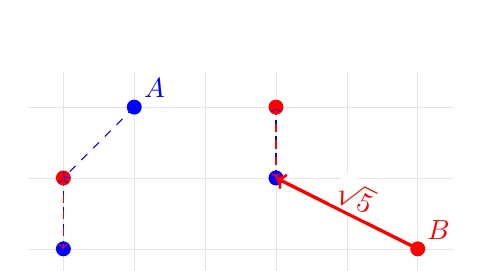
\begin{tikzpicture}[scale=0.9]
    \draw[step=1cm, gray!20, very thin] (-0.5,-0.5) grid (5.5,2.5);
    \fill[blue] (0,0) circle (3pt);
    \fill[blue] (1,2) circle (3pt);
    \fill[blue] (3,1) circle (3pt);
    \fill[red] (0,1) circle (3pt);
    \fill[red] (3,2) circle (3pt);
    \fill[red] (5,0) circle (3pt);
    \draw[->, blue, dashed] (0,0) -- (0,1);
    \draw[->, blue, dashed] (1,2) -- (0,1);
    \draw[->, blue, dashed] (3,1) -- (3,2);
    \draw[->, red, dashed] (0,1) -- (0,0);
    \draw[->, red, dashed] (3,2) -- (3,1);
    \draw[->, red, very thick] (5,0) -- (3,1)
        node[midway, above, sloped, fill=white, inner sep=1pt] {$\sqrt{5}$};
    \node[blue, above right] at (1,2) {$A$};
    \node[red, above right] at (5,0) {$B$};
\end{tikzpicture}
\caption{Nearest-neighbour arrows between two point sets. The longest arrow has length $\sqrt{5}$ and realises $d_{\mathrm{Hau}}(A,B)$.}
\label{fig:hausdorff-points}
\end{figure}

\begin{example}[Sensitivity to a single outlier]
    Let $A=[0,2]\times[0,2]$ be a filled square and let $B=A\cup\{(3,1)\}$ add one point one unit to its right, as in Figure~\ref{fig:hausdorff-outlier}. Every point of $A$ already belongs to $B$, so $d(A,B)=0$. The extra point of $B$ is at distance $1$ from $A$, hence $d(B,A)=1$ and $d_{\mathrm{Hau}}(A,B)=1$. A single outlier therefore determines the whole distance, even though the two sets overlap almost completely.
\end{example}

\begin{figure}[htbp]
\centering
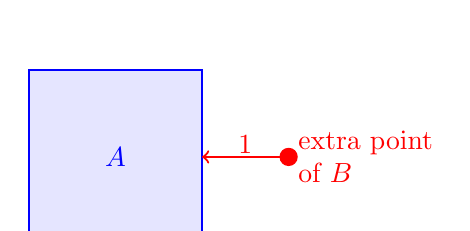
\begin{tikzpicture}[scale=1.1]
    \draw[fill=blue!10, draw=blue, thick] (0,0) rectangle (2,2);
    \fill[red] (3,1) circle (3pt);
    \draw[->, red, thick] (3,1) -- (2,1)
        node[midway, above, fill=white, inner sep=1pt] {$1$};
    \node[blue] at (1,1) {$A$};
    \node[red, right, align=left] at (3,1) {extra point\\of $B$};
\end{tikzpicture}
\caption{Adding one outlier at distance $1$ makes $d_{\mathrm{Hau}}(A,B)=1$; the Hausdorff distance measures worst-case, not average, disagreement.}
\label{fig:hausdorff-outlier}
\end{figure}

\begin{example}[A finite sample of an interval]
    Take $A=[0,1]\subset\mathbb{R}$ and the grid $B=\{0,\tfrac14,\tfrac12,\tfrac34,1\}$. Every point of $B$ lies in $A$, so $d(B,A)=0$. A point of $A$ is at most half a grid spacing away from $B$, attained midway between adjacent grid points, so $d(A,B)=1/8$ and $d_{\mathrm{Hau}}(A,B)=1/8$. More generally, a uniform sample of mesh size $h$ approximates the interval within Hausdorff distance $h/2$.
\end{example}

\emph{Applications.} Hausdorff distance compares shapes rather than corresponding points, because it does not require the two sets to have the same cardinality or parametrisation. It is used to evaluate image segmentations by measuring the distance from a predicted boundary to the ground-truth boundary, to compare point clouds in 3D registration and LiDAR scanning, and to quantify the error introduced by simplifying a mesh. Its worst-case nature makes it sensitive to isolated errors, as in Figure~\ref{fig:hausdorff-outlier}, so practical loss functions often use a trimmed or averaged (Chamfer) variant instead.

\coderef{Code/distance_metrics.ipynb}  
\coderef{Code/probability_distances.ipynb}
\coderef{Code/knn_tutorial.ipynb}

\chapter{Probability Review}
\label{ch:prob}

\section{Random variables and distributions}

\begin{epigraph}
    {You can, for example, never foretell what any one man will do, but you can say with precision what an average number will be up to. Individuals vary, but percentages remain constant. So says the statisticians.}{Sherlock Holmes, The Sign of Four}
\end{epigraph}

This chapter delves into the critical role of statistics and probability in machine learning, starting with an overview of random experiments and variables. It progresses to cover essential topics such as set theory, probability, conditional probability, and key theorems such as the Bayes Theorem and the Central Limit Theorem (CLT). The discussion extends to distribution functions, the significance of expected values and variance,
and the normal distribution, along with a variety of other distributions relevant to ML.The chapter also introduces Moment Generating Functions as vital tools in probability theory, providing a foundation for understanding the CLT's implications for data analysis and prediction in machine learn-
ing. By exploring these statistical concepts, the chapter aims to equip readers with the necessary knowledge to effectively engage with machine learning models and understand the statistical underpinnings of algorithm performance and data analysis.

\begin{definition}[Random Experiment, Outcome Space, Event]
    Experiments for which the outcome cannot be predicted with certainty are called \emph{random experiments}\index{random experiments}. The collection of all possible outcomes of a random experiment is called the \emph{outcome space}\index{outcome space} and is indicated with $S$. An event $A$ is a subset of the outcome space $S$.
\end{definition}

\begin{example}[Coin toss]
    Toss a fair coin once. The outcome space is $S=\{\mathrm{H},\mathrm{T}\}$. The set $A=\{\mathrm{H}\}$ (``heads'') is an event, and so are $\{\mathrm{T}\}$ and $S$ itself.
\end{example}

\begin{example}[Die roll]
    Roll a six-sided die. Here $S=\{1,2,3,4,5,6\}$, and $A=\{2,4,6\}$ is the event ``the result is even''.
\end{example}

\begin{example}[Drawing a card]
    Draw one card from a standard deck. The outcome space is the set of all $52$ cards, and the $13$ hearts form an event.
\end{example}

\begin{definition}[Random variable]
    A \emph{random variable}\index{random variable} $X$ is a function from a sample space $S$ to the real numbers: $X : S \to \mathbb{R}$.
\end{definition}

\begin{example}[Bernoulli variable]
    For the coin toss define $X(\mathrm{H})=1$ and $X(\mathrm{T})=0$. Then $X$ is a Bernoulli random variable encoding the number of heads.
\end{example}

\begin{example}[Indicator of parity]
    For the die roll, $X(s)=s$ maps each face to its numerical value, while $Y(s)=\mathbf{1}_{\{s \text{ even}\}}$ indicates parity.
\end{example}

\begin{example}[Continuous measurement]
    Measure the height of a uniformly chosen student from a class. The map from the student (the outcome) to a real number of centimetres is a random variable.
\end{example}

\begin{definition}[Mutually exclusive events]
    Given an outcome space $S$, we call mutually exclusive events $A_i$ with $i=1,\ldots,k$ (we consider here only a finite set of
events) when 
\begin{align}
    A_i \cap A_j = \varnothing, \qquad i \neq j.
\end{align}
\end{definition}
\begin{example}[Coin toss]
    In a coin toss, $A_1=\{\mathrm{H}\}$ and $A_2=\{\mathrm{T}\}$ are mutually exclusive: $A_1\cap A_2=\varnothing$.
\end{example}

\begin{example}[Die roll]
    In a die roll, $A_1=\{1,2\}$, $A_2=\{3,4\}$ and $A_3=\{5,6\}$ are pairwise disjoint.
\end{example}

\begin{example}[Drawing a card]
    When drawing one card, the events ``heart'' and ``spade'' cannot occur simultaneously, so they are mutually exclusive.
\end{example}

\begin{definition}[Exhaustive events]
    Given an outcome space $S$, we call exhaustive
events $A_i$ with $i= 1,\ldots,k$ (we consider here only a finite set of events) when
\begin{align}
    \bigcup_{i=1}^k A_i = S
\end{align}
\end{definition}
\begin{example}[Coin toss]
    For the coin toss, $\{\mathrm{H}\}\cup\{\mathrm{T}\}=S$, so the two singleton events are exhaustive.
\end{example}

\begin{example}[Die roll]
    For the die roll, $\{1,2,3\}\cup\{4,5,6\}=S$: the events ``low'' and ``high'' exhaust the space.
\end{example}

\begin{example}[Drawing a card]
    The four suit events partition a deck of cards, so they are exhaustive (and mutually exclusive).
\end{example}

Suppose we repeat an experiment $n$ times and we count the number of times we observe event $A$ as output. We indicate this number with $m(A)$. Note that naturally, even if not explicitly indicated, $m(A)$ is dependent on $n$.

\begin{definition}
    The \emph{relative frequency} of event $A$ is defined as
    \begin{align}
        p_n(A) = \frac{m(A)}{n}
    \end{align}
    Note that this is rather rapidly varying numbers in practice, but that it tends to vary less as $n$ grows. We can define
    \begin{align}
         p(A) &\defn \lim_{n \rightarrow \infty} \frac{m(A)}{n}
     \end{align}
\end{definition}
\begin{example}[Coin toss]
    Toss a fair coin $n=1000$ times and observe $m(\mathrm{H})=497$. Then $p_n(\mathrm{H})=0.497$, close to the limiting probability $p(\mathrm{H})=0.5$.
\end{example}

\begin{example}[Die roll]
    Roll a die $n$ times; the relative frequency $p_n(\{6\})$ converges to $\dfrac{1}{6}$ as $n\to\infty$, although it fluctuates noticeably for small $n$.
\end{example}

\begin{example}[Spam filtering]
    If $23$ of the first $100$ emails are spam, $p_{100}(\text{spam})=0.23$; with more messages this estimate stabilises around the true spam rate.
\end{example}

\begin{definition}
     A collection $\mathcal{Q}$ of subsets of $S$ is called a $\sigma$-algebra if it satisfies the following three properties:
\begin{enumerate}
    \item The empty set $\varnothing \in \mathcal{Q}$.
    \item If $A \in \mathcal{Q}$, then $A^c \in \mathcal{Q}$.
    \item If $A_1, A_2, \ldots \in \mathcal{Q}$, then 
    \begin{align}
        \bigcup_{i=1}^\infty A_i \in \mathcal{Q}    
    \end{align}
\end{enumerate}
\end{definition}

\begin{example}[Trivial $\sigma$-algebra]
    The collection $\mathcal{Q}=\{\varnothing,S\}$ is a $\sigma$-algebra for any outcome space $S$.
\end{example}

\begin{example}[Power set]
    For $S=\{\mathrm{H},\mathrm{T}\}$, the power set $\{\varnothing,\{\mathrm{H}\},\{\mathrm{T}\},S\}$ is a $\sigma$-algebra.
\end{example}

\begin{example}[A non-example]
    For $S=\{1,2,3,4\}$, $\mathcal{Q}=\{\varnothing,\{1,2\},\{3,4\},S\}$ is a $\sigma$-algebra, while $\{\varnothing,\{1,2\},S\}$ is not: the complement of $\{1,2\}$ is missing.
\end{example}

\begin{definition}
      Given a sample space $S$ and an associated $\sigma$-algebra $\mathcal{Q}$, a \emph{probability function}\index{probability function} $\Pr(A)$ with domain $\mathcal{Q}$ is a real-valued set function $\Pr: \mathcal{Q} \to \mathbb{R}$ such that
     \begin{enumerate}
         \item $\Pr(A) \geq 0$ for all $A \in \mathcal{Q}$,
         \item $\Pr(S) = 1$,
         \item if $A_i \in \mathcal{Q}$ and $A_i \cap A_j = \emptyset$ for $i \neq j$ (mutually exclusive events), then
         $$\Pr\left(\bigcup_{i=1}^\infty A_i\right) = \sum_{i=1}^\infty \Pr(A_i).$$
     \end{enumerate}
\end{definition}
Note that the three properties given in the definition are referred as the axioms of probability or the \emph{Kolmogorov axioms}\index{Kolmogorov axioms}. 
\begin{example}[Fair coin]
    For a fair coin, $\Pr(\{\mathrm{H}\})=\Pr(\{\mathrm{T}\})=1/2$ and $\Pr(S)=1$; the axioms give $\Pr(\varnothing)=0$.
\end{example}

\begin{example}[Fair die]
    For a fair die, $\Pr(\{i\})=1/6$ for each $i$, hence $\Pr(\{2,4,6\})=1/2$ by additivity.
\end{example}

\begin{example}[Continuous uniform]
    The uniform distribution on $[0,1]$ assigns $\Pr([a,b])=b-a$: length is non-negative, $\Pr([0,1])=1$, and disjoint intervals add.
\end{example}

\begin{definition}
    Given two events $A$ and $B$, they are said to be independent if and only if
    \begin{align}
        \Pr(A \cap B) = \Pr(A)\Pr(B)
    \end{align}
\end{definition}

\begin{example}[Two coin tosses]
    Toss a fair coin twice. Let $A$ be ``heads first'' and $B$ ``heads second''. Then $\Pr(A\cap B)=1/4=\Pr(A)\Pr(B)$, so $A$ and $B$ are independent.
\end{example}

\begin{example}[Different experiments]
    Roll a die and toss a coin. The event ``die shows $6$'' and the event ``coin shows heads'' are independent because the two experiments do not influence one another.
\end{example}

\begin{example}[With and without replacement]
    Draw two cards \emph{with} replacement: their colours are independent. Without replacement they are dependent, since $\Pr(\text{second red}\mid\text{first red})=25/51\neq 1/2$.
\end{example}

\begin{theorem}
    Let $S = \{s_1, \ldots, s_n\}$ be a finite set. Let $\mathcal{Q}$ be any $\sigma$-algebra of subsets of $S$. Let $p_1, \ldots, p_n$ be positive real numbers such that $\sum_{i=1}^n p_i = 1$. For any $A \in \mathcal{Q}$, define $\Pr(A)$ by
    \begin{align}
        \Pr(A) &\defn \sum_{s_i \in A} p_i
    \end{align}
    Then $\Pr$ is a probability function on $\mathcal{Q}$. This remains true if $S$ is a countable set.
\end{theorem}
\begin{proof}
    Non-negativity is immediate: since $p_i>0$ for every $i$, $\Pr(A)=\sum_{s_i\in A}p_i\geq 0$ for all $A\in\mathcal{Q}$.
    Normalisation follows from $\Pr(S)=\sum_{i=1}^n p_i=1$.
    For countable additivity, let $A_1,A_2,\ldots\in\mathcal{Q}$ be pairwise disjoint. Because all terms are non-negative, the series may be rearranged:
    \begin{align}
        \Pr\left(\bigcup_{j=1}^\infty A_j\right)
        &= \sum_{s_i \in \bigcup_j A_j} p_i\\
        &= \sum_{j=1}^\infty\ \sum_{s_i \in A_j} p_i\\
        &= \sum_{j=1}^\infty \Pr(A_j).
    \end{align}
    The rearrangement is legitimate because disjointness ensures each $s_i$ belongs to at most one $A_j$. The identical argument applies when $S$ is countable.
\end{proof}

\begin{example}[Weighted die]
    For $S=\{1,\ldots,6\}$ with $p_i = \dfrac{i}{21}$ (these weights sum to $1$), the probability of an even face is 
    \begin{align}
        \Pr(\{2,4,6\}) &= \frac{2+4+6}{21} \\
        &= \frac{12}{21} \\
        &= \frac{4}{7}.
    \end{align}
\end{example}

\begin{example}[Uniform finite choice]
    Choosing a name uniformly from a list of $n$ students corresponds to
    \begin{align}
        p_i &= \frac{1}{n}
    \end{align}
    any subset $A$ of size $m$ then has probability $\dfrac{m}{n}$.
\end{example}

\begin{example}[Biased coin]
    A biased coin with $p_{\mathrm{H}}=0.7$ and $p_{\mathrm{T}}=0.3$ is the finite model underlying a Bernoulli trial.
\end{example}

\begin{definition}
    Given a vector $\mathbf{v} = (v_1, \ldots, v_n)$
with $n$ some integer the softmax function is a function $\mathrm{SM}: \mathbb{R}^n \longrightarrow \mathbb{R}^n$ that gives as output for its $i$th component
\begin{align}
    \mathrm{SM}(\mathbf{v})_i &\defn  \frac{e^{v_i}}{\displaystyle  \sum_{j=1}^n e^{v_j}}
\end{align}
\end{definition}

\begin{example}[Three logits]
    For $\mathbf{v}=(1,2,3)$, $\mathrm{SM}(\mathbf{v})\approx(0.090,0.245,0.665)$. The largest logit receives the largest probability, and the components sum to $1$.
\end{example}

\begin{example}[Shift invariance]
    Adding a constant to every logit leaves softmax unchanged: 
    \begin{align}
        \mathrm{SM}(\mathbf{v}+c\mathbf{1})=\mathrm{SM}(\mathbf{v})
    \end{align}
    Numerical implementations therefore subtract $\max_i v_i$ before exponentiating.
\end{example}

\begin{example}[Multiclass classification]
    In multiclass logistic regression the model outputs logits $f_1(\mathbf{x}),\ldots,f_k(\mathbf{x})$ and predicts class $i$ with probability $\mathrm{SM}(\mathbf{f}(\mathbf{x}))_i$.
\end{example}

\begin{definition}[\emph{probability mass function}]
    The probability massfunction (PMF) of a discrete random variable $X$ is defined by
    \begin{align}
        f_X(x) &\defn \Pr(X=x)
    \end{align}
    In this case it is easy to see that
    \begin{align}
        F_X(x) &\defn \Pr(X \leq x) = \sum_{x' \leq x} f_X(x')
    \end{align}
    assuming that the discrete random variable $X$ can only assume a finite set of $N$ values indicated by $x_k$ with $k=1,\ldots,N$, and $A=\{k \mid x_k \leq x\}$, so $F_X(x)=\sum_{k \in A} f_X(x_k)$.
\end{definition}
\begin{example}[Bernoulli PMF]
    For $X\sim\mathrm{Bernoulli}(p)$ the mass function is $f_X(1)=p$, $f_X(0)=1-p$, and $f_X(x)=0$ otherwise. The CDF is the step function $F_X(x)=0$ for $x<0$, $1-p$ for $0\leq x<1$, and $1$ for $x\geq1$.
\end{example}

\begin{example}[Fair die]
    For a fair die, $f_X(k)=1/6$ for $k=1,\ldots,6$. Hence $F_X(3.5)=\sum_{k=1}^3 1/6=1/2$, illustrating that the CDF is piecewise constant between the attainable values.
\end{example}

\begin{example}[Binomial PMF]
    If $X\sim\mathrm{Binomial}(n,p)$ counts successes in $n$ independent trials, then $f_X(k)=\binom{n}{k}p^k(1-p)^{n-k}$ for $k=0,\ldots,n$, and these masses sum to $1$ by the binomial theorem.
\end{example}

\begin{definition}
The probability density function (PDF) $f_X(x)$ of a continuous random variable $X$ is the function $f_X(x)$ that satisfy
\begin{align}
    F_X(x) = \int_{-\infty}^x f_X(t)\,dt
\end{align}
for all $x$.
\end{definition}
\begin{example}[Uniform density]
    For $X\sim\mathrm{Unif}[0,1]$, $f_X(x)=1$ on $[0,1]$ and $0$ elsewhere. Then $F_X(x)=\int_0^x dt=x$ for $0\leq x\leq1$, with $F_X(x)=0$ below $0$ and $1$ above $1$.
\end{example}

\begin{example}[Exponential density]
    If $f_X(x)=\lambda e^{-\lambda x}$ for $x\geq0$, then $F_X(x)=\int_0^x\lambda e^{-\lambda t}dt=1-e^{-\lambda x}$. This is the waiting time until the first event of a Poisson process.
\end{example}

\begin{example}[Standard normal density]
    The standard normal density $\phi(x)=\frac{1}{\sqrt{2\pi}}e^{-x^2/2}$ integrates to $1$ (the Gaussian integral), so it is a valid PDF; its CDF $\Phi(x)=\int_{-\infty}^x\phi(t)dt$ has no elementary closed form.
\end{example}

\begin{theorem}
    A function $f_X(x)$ is a probability density function if and only if
    \begin{enumerate}
        \item $f_X(x) \geq 0$ for all $x$, and
        \item $\int_{-\infty}^\infty f_X(x)\,dx = 1$.
    \end{enumerate}
\end{theorem}
\begin{proof}
    ($\Rightarrow$) If $f_X$ is a density, then $F_X(x)=\int_{-\infty}^x f_X(t)dt$ is non-decreasing, which forces $f_X(x)\geq0$ wherever the derivative exists. Taking $x\to\infty$ gives $\int_{-\infty}^\infty f_X(t)dt=\lim_{x\to\infty}F_X(x)=1$.
    ($\Leftarrow$) Conversely, if $f_X\geq0$ and $\int f_X=1$, define $F(x)=\int_{-\infty}^x f_X(t)dt$. Then $F$ is non-decreasing, $\lim_{x\to-\infty}F(x)=0$ and $\lim_{x\to\infty}F(x)=1$, so $F$ is a valid CDF and $f_X$ is its density.
\end{proof}
\begin{example}[Uniform over unit interval]
    $f(x)=1$ for $0\leq x\leq1$ and $0$ otherwise is non-negative and integrates to $1$, hence a PDF.
\end{example}

\begin{example}[Triangular density]
    $f(x)=2x$ on $[0,1]$ is non-negative and $\int_0^1 2x\,dx=1$; it is a valid density that concentrates mass near $1$.
\end{example}

\begin{example}[A non-example]
    $g(x)=x$ on $[0,2]$ is non-negative but $\int_0^2 x\,dx=2\neq1$, so it cannot be a density; rescaling to $g(x)=x/2$ fixes it.
\end{example}

\section{Expectation, variance, and covariance}

\begin{definition}
    The \emph{expected value} of a discrete random variable is
\begin{align}
    \E[X] &\defn \sum_x x \, \Pr(X = x),
\end{align}
and for a continuous random variable with density $p_X$,
\begin{align}
    \E[X] = \int x \, p_X(x) \, dx.
\end{align}
\end{definition}
\begin{example}[Expectation of a die roll]
    For a fair six-sided die, $X\in\{1,\ldots,6\}$ with $\Pr(X=k)= \dfrac{1}{6}$. Thus
    \begin{align}
        \E[X] = \sum_{k=1}^6 k\cdot\frac16
        = \frac{1+2+3+4+5+6}{6} = \frac{21}{6} = 3.5.
    \end{align}
    The mean need not be a value that the variable can actually take.
\end{example}

\begin{example}[Expectation of an exponential variable]
    For $X\sim\mathrm{Exp}(\lambda)$ (the notation $X\sim\mathscr{D}$ means that $X$ is distributed according to $\mathscr{D}$) with density
    $p_X(x)=\lambda e^{-\lambda x}$ on $x\geq0$,
    \begin{align}
        \E[X] = \int_0^\infty x\,\lambda e^{-\lambda x}\,dx
        = \frac{1}{\lambda},
    \end{align}
    which follows by integrating by parts. A larger $\lambda$ means a shorter
    typical waiting time.
\end{example}

\begin{proposition}
    Linearity of expectation holds regardless of independence:
    \begin{align}
        \E[aX + bY] = a\E[X] + b\E[Y].
    \end{align}
\end{proposition}
\begin{proof}
    Consider the discrete case and write $p(x,y)=\Pr(X=x,Y=y)$. Then
    \begin{align}
        \E[aX+bY]
        &= \sum_x\sum_y (ax+by)\,p(x,y)\\
        &= a\sum_x x\sum_y p(x,y) + b\sum_y y\sum_x p(x,y)\\
        &= a\sum_x x\,\Pr(X=x) + b\sum_y y\,\Pr(Y=y)\\
        &= a\,\E[X] + b\,\E[Y].
    \end{align}
    The first equality uses the joint mass function, the second rearranges the finite sums, and the third uses the marginalisation identities
    \begin{align}
        \sum_y p(x,y) &= \Pr(X=x) \\
        \sum_x p(x,y) &= \Pr(Y=y).
    \end{align}
    The continuous case is identical with sums replaced by integrals. Independence is never used, so the result holds for any pair of random variables with finite expectations.
\end{proof}
\begin{example}[Sum of two dice]
    Let $X_1$ and $X_2$ be the outcomes of two fair dice. Linearity gives
    \begin{align}
        \E[X_1+X_2] = \E[X_1]+\E[X_2]
        = 3.5+3.5 = 7.
    \end{align}
    We do not need to enumerate the $36$ equally likely pairs, and the result
    does not rely on the dice being independent.
\end{example}

\begin{example}[Expectation of a binomial variable]
    If $X\sim\mathrm{Binomial}(n,p)$, write $X=\sum_{i=1}^n X_i$ where $X_i$ is
    the indicator that trial $i$ succeeds. Each $X_i$ is Bernoulli with mean $p$,
    so linearity gives
    \begin{align}
        \E[X] = \sum_{i=1}^n \E[X_i] = np.
    \end{align}
    This is much simpler than summing $k\binom{n}{k}p^k(1-p)^{n-k}$ over all $k$.
\end{example}

\begin{example}[The sample mean is unbiased]
    For independent observations $X_1,\ldots,X_n$ with common mean $\mu$, the
    sample mean $\bar X = \frac1n\sum_{i=1}^n X_i$ satisfies
    \begin{align}
        \E[\bar X]
        = \frac1n\sum_{i=1}^n \E[X_i]
        = \frac1n\cdot n\mu = \mu.
    \end{align}
    Linearity is the only property needed for unbiasedness; independence is not
    required here, although it is needed to compute the variance of $\bar X$.
\end{example}

\begin{definition}
        The \emph{variance} measures spread about the mean:
\begin{align}
    \Var(X) = \E[(X - \E[X])^2] = \E[X^2] - \E[X]^2.
\end{align}
\end{definition}

\begin{example}[Variance of a die roll]
    For a fair die, $\E[X^2]=\frac{1^2+\cdots+6^2}{6}=\frac{91}{6}$, so $\Var(X)=\frac{91}{6}-\left(\frac72\right)^2=\frac{35}{12}\approx2.92$.
\end{example}

\begin{example}[Variance of a uniform variable]
    For $X\sim\mathrm{Unif}[a,b]$, $\E[X]=(a+b)/2$ and $\E[X^2]=(a^2+ab+b^2)/3$, giving $\Var(X)=(b-a)^2/12$.
\end{example}

\begin{example}[Variance of a Gaussian]
    If $X\sim\mathscr{N}(\mu,\sigma^2)$, then by definition $\Var(X)=\sigma^2$; the parameter $\sigma$ is the standard deviation, the natural scale of the fluctuations about $\mu$.
\end{example}

\begin{definition}
    The \emph{covariance} of random variables $X$ and $Y$ is defined as:
\begin{align}
    \Cov(X,Y) = \E[(X-\E[X])(Y-\E[Y])] = \E[XY] - \E[X]\E[Y],
\end{align}
It measures joint variation.
\end{definition}
\begin{example}[Independent variables]
    If $X$ and $Y$ are independent, $\E[XY]=\E[X]\E[Y]$, hence $\Cov(X,Y)=0$.
\end{example}

\begin{example}[Perfect positive dependence]
    Taking $Y=X$ gives $\Cov(X,X)=\Var(X)$ and correlation $1$.
\end{example}

\begin{example}[Perfect negative dependence]
    Taking $Y=-X$ gives $\Cov(X,Y)=-\Var(X)$ and correlation $-1$.
\end{example}

\begin{example}[Variance of a Bernoulli variable]
    For $X\sim\mathrm{Bernoulli}(p)$, $X^2=X$ because $X$ takes only the values
    $0$ and $1$. Hence $\E[X^2]=p$ and
    \begin{align}
        \Var(X) = \E[X^2]-\E[X]^2 = p-p^2 = p(1-p).
    \end{align}
    The variance is largest at $p=1/2$ and vanishes at $p=0$ and $p=1$.
\end{example}

\begin{proposition}
    The variance satisfies the following properties:
    \begin{enumerate}
        \item $\Var(X) \geq 0$.
        \item $\Var(a) = 0$ for any constant $a$.
        \item $\Var(X + a) = \Var(X)$ for any constant $a$.
        \item $\Var(aX) = a^2\Var(X)$ for any constant $a$.
        \item $\Var(aX+bY) = a^2\Var(X)+b^2\Var(Y)+2ab\Cov(X,Y)$.
    \end{enumerate}
\end{proposition}
\begin{proof}
    (1) $\Var(X)=\E[(X-\E[X])^2]\geq0$ because squares are non-negative.
    (2) For a constant $a$, $\E[a]=a$, so $\Var(a)=\E[(a-a)^2]=0$.
    (3) $\Var(X+a)=\E[(X+a-\E[X]-a)^2]=\Var(X)$.
    (4) $\Var(aX)=\E[(aX-a\E[X])^2]=a^2\Var(X)$.
    (5) Writing $\tilde X=X-\E[X]$ and $\tilde Y=Y-\E[Y]$,
    \begin{align}
        \Var(aX+bY)&=\E[(a\tilde X+b\tilde Y)^2]\\
        &=a^2\E[\tilde X^2]+b^2\E[\tilde Y^2]+2ab\,\E[\tilde X\tilde Y]\\
        &=a^2\Var(X)+b^2\Var(Y)+2ab\,\Cov(X,Y).\qedhere
    \end{align}
\end{proof}

\begin{definition}
    The \emph{correlation} between random variables $X$ and $Y$ is defined as:\begin{align}
    \rho_{XY} = \Cov(X,Y)/\sqrt{\Var(X)\Var(Y)} \in [-1,1].
\end{align}
\end{definition}
\begin{example}[Perfect positive correlation]
    If $Y=X$ with $\Var(X)>0$, then $\rho_{XY}=\Var(X)/\Var(X)=1$.
\end{example}

\begin{example}[Perfect negative correlation]
    If $Y=-X$, then $\rho_{XY}=-\Var(X)/\Var(X)=-1$: the two variables move in exactly opposite directions.
\end{example}

\begin{example}[Uncorrelated but dependent]
    Independence gives $\Cov(X,Y)=0$ and hence $\rho_{XY}=0$; the converse fails, e.g.\ $X\sim\mathrm{Unif}[-1,1]$ and $Y=X^2$ are dependent but uncorrelated.
\end{example}

\begin{example}[Affine transformations and sums]
    For constants $a,b$,
    \begin{align}
        \Var(aX+b) &= a^2\Var(X),\\
        \Var(X+Y) &= \Var(X)+\Var(Y)+2\Cov(X,Y).
    \end{align}
    Adding a constant does not change the spread, multiplying by $a$ scales the variance by $a^2$, and variances add exactly when $\Cov(X,Y)=0$. Independent
    variables have zero covariance, but the converse is false in general.
\end{example}

\begin{example}[Computing a correlation]
    Let $X$ and $Y$ be binary with joint probabilities
    $\Pr(0,0)=0.4$, $\Pr(0,1)=0.1$, $\Pr(1,0)=0.1$, and $\Pr(1,1)=0.4$. Then
    $\E[X]=\E[Y]=0.5$ and $\E[XY]=\Pr(1,1)=0.4$, so
    \begin{align}
        \Cov(X,Y) &= 0.4-0.5\cdot0.5 = 0.15,\\
        \Var(X)=\Var(Y) &= 0.5-0.25 = 0.25.
    \end{align}
    Therefore $\rho_{XY}=0.15/0.25=0.6$: the variables are positively but not
    perfectly correlated.
\end{example}

\begin{definition}
    For a random vector $X$, the \emph{covariance matrix}\index{covariance matrix} is
\begin{align}
    \Sigma = \E[(\vec{X}-\vec{\mu})(\vec{X}-\vec{\mu})^\top].
\end{align}
\end{definition}
\begin{example}[Independent coordinates]
    If $X_1$ and $X_2$ are independent with unit variance, then $\Sigma=I_2$: zero off-diagonal entries record the absence of linear dependence.
\end{example}

\begin{example}[Binary variables]
    For the binary pair with joint masses $0.4,0.1,0.1,0.4$ from the correlation example, $\Sigma=\begin{bmatrix}0.25&0.15\\0.15&0.25\end{bmatrix}$.
\end{example}

\begin{example}[Rescaling a coordinate]
    If $Y=2X$ and $\Var(X)=1$, the vector $(X,Y)$ has covariance matrix $\begin{bmatrix}1&2\\2&4\end{bmatrix}$; the correlation remains $1$.
\end{example}

\begin{example}[From covariance matrix to correlation matrix]
    Suppose $\Var(X_1)=4$, $\Var(X_2)=9$, and $\Cov(X_1,X_2)=3$. The covariance
    matrix is
    \begin{align}
        \Sigma =
        \begin{bmatrix}4&3\\3&9\end{bmatrix},
    \end{align}
    and the correlation is $\rho=3/\sqrt{4\cdot9}=3/6=0.5$. Dividing each entry
    by the corresponding standard deviations gives the correlation matrix
    \begin{align}
        R =
        \begin{bmatrix}1&0.5\\0.5&1\end{bmatrix}.
    \end{align}
    The diagonal of $\Sigma$ carries the scales, while $R$
    removes them.
\end{example}

\begin{proposition}
    If $\vec{Y}=A \vec{X}+\vec{b}$, then
    \begin{align}
        \Sigma_{\vec{Y}}
        = A\,\Sigma_{\vec{X}}\,A^\top.
    \end{align}
\end{proposition}
\begin{proof}
    Let $\vec\mu=\E[\vec X]$. Since $\E[\vec Y]=A\vec\mu+\vec b$, the constant $\vec b$ cancels in the centred vector:
    \begin{align}
        \Sigma_{\vec Y}&=\E\!\left[(\vec Y-\E\vec Y)(\vec Y-\E\vec Y)^\top\right]\\
        &=\E\!\left[A(\vec X-\vec\mu)(\vec X-\vec\mu)^\top A^\top\right]\\
        &=A\,\Sigma_{\vec X}\,A^\top,
    \end{align}
    where $A$ and $A^\top$ are deterministic and may be pulled outside the expectation.
\end{proof}

\begin{example}[Covariance under a linear transformation]
    Let
    $\Sigma_{X}=\begin{bmatrix}2&1\\1&2\end{bmatrix}$
    and $A=\begin{bmatrix}1&1\\1&-1\end{bmatrix}$,
    \begin{align}
        A\Sigma_{X}A^\top
        = \begin{bmatrix}6&0\\0&2\end{bmatrix}.
    \end{align}
    The transformed coordinates are uncorrelated even though the original ones
    were not.
\end{example}

\begin{example}[A singular covariance matrix]
    Let $X_1$ and $X_2$ be independent with unit variance, and let
    $X_3=X_1+X_2$. Then
    \begin{align}
        \Cov(X_1,X_3)=\Cov(X_1,X_1)+\Cov(X_1,X_2)=1,
    \end{align}
    and similarly $\Cov(X_2,X_3)=1$, while
    $\Var(X_3)=\Var(X_1)+\Var(X_2)=2$. Hence
    \begin{align}
        \Sigma =
        \begin{bmatrix}1&0&1\\0&1&1\\1&1&2\end{bmatrix},
    \end{align}
    which has rank two: the vector $(1,1,-1)^\top$ lies in its null space because
    $X_3-X_1-X_2=0$. Singular covariance matrices signal an exact linear
    dependence among the features.
\end{example}

\begin{example}[Variance along a direction]
    For a unit vector $\vec u$, the variance of the projection $\vec u^\top\vec X$ equals $\vec u^\top\Sigma\vec u$; the principal axes of the ellipsoid $\vec x^\top\Sigma^{-1}\vec x=\mathrm{const}$ are the eigenvectors of $\Sigma$.
\end{example}

\begin{example}[Variance of a sum]
    For $\vec 1=(1,1)^\top$, $\Var(X_1+X_2)=\vec 1^\top\Sigma\vec 1=\Var(X_1)+\Var(X_2)+2\Cov(X_1,X_2)$.
\end{example}

\begin{example}[Diagonalisation]
    If $\Sigma=Q\Lambda Q^\top$ with $Q$ orthogonal, the change of coordinates $\vec Z=Q^\top\vec X$ has diagonal covariance $\Lambda$; the transformed features are uncorrelated.
\end{example}

\section{Associated distributions}

\begin{definition}
    The \emph{joint distribution}\index{joint distribution} of two random variables $X, Y$ is
$\Pr(X = x, Y = y)$. The \emph{marginal distribution}\index{marginal distribution} is obtained by summing (or integrating) out the other variable:
\begin{align}
    \Pr(X = x) = \sum_y \Pr(X = x, Y = y).
\end{align}
\end{definition}
\begin{example}[Two coin tosses]
    For two fair tosses, $\Pr(X=\mathrm{H},Y=\mathrm{H})=1/4$ for each of the four pairs. Marginalising, $\Pr(X=\mathrm{H})=\sum_y\Pr(X=\mathrm{H},Y=y)=1/2$.
\end{example}

\begin{example}[Two dice]
    Let $X$ be the first die and $S$ the sum of two dice. The joint mass satisfies $\Pr(X=x,S=s)=\Pr(X=x)\Pr(Y=s-x)=1/36$ whenever $1\leq s-x\leq6$; summing over $s$ recovers $\Pr(X=x)=1/6$.
\end{example}

\begin{example}[Continuous uniform on a square]
    If $(X,Y)$ is uniform on $[0,1]^2$, the joint density is $f(x,y)=1$ there. The marginal $f_X(x)=\int_0^1 f(x,y)\,dy=1$, so each coordinate is uniform on $[0,1]$.
\end{example}

\begin{definition}
    The \emph{conditional distribution}\index{conditional distribution} is
    \begin{align}
        \Pr(Y = y \mid X = x) = \frac{\Pr(X = x, Y = y)}{\Pr(X = x)},
        \qquad \Pr(X=x) > 0.
    \end{align}
\end{definition}
\begin{example}[Coin tosses]
    For two fair tosses, $\Pr(Y=\mathrm{H}\mid X=\mathrm{H})=\frac{\Pr(X=\mathrm{H},Y=\mathrm{H})}{\Pr(X=\mathrm{H})}=\frac{1/4}{1/2}=1/2$; knowing the first toss does not change the second.
\end{example}

\begin{example}[Die roll]
    For a fair die, $\Pr(X\text{ even}\mid X>3)=\Pr(\{4,6\})/\Pr(\{4,5,6\})=(2/6)/(3/6)=2/3$.
\end{example}

\begin{example}[Spam filtering]
    If $10\%$ of messages are spam and $50\%$ of spam but only $5\%$ of legitimate messages contain ``free'', then $\Pr(\text{spam}\mid\text{``free''})=\frac{0.5\cdot0.1}{0.5\cdot0.1+0.05\cdot0.9}\approx0.53$.
\end{example}

\section{Bayes' rule}

\begin{proposition}
    Let $X$ and $Y$ be random variables. Then
    \begin{align}
    \Pr(Y = y \mid X = x)
    = \frac{\Pr(X = x \mid Y = y) \, \Pr(Y = y)}{\Pr(X = x)}.
\end{align}
\end{proposition}

The denominator is a normalising constant: $\Pr(X=x) = \sum_{y'} \Pr(X=x \mid Y=y')\Pr(Y=y')$. In Bayesian terminology, $\Pr(Y=y)$ is the \emph{prior}, $\Pr(X=x\mid Y=y)$ the \emph{likelihood}, and $\Pr(Y=y\mid X=x)$ the \emph{posterior}.

The random variables $X$ and $Y$ are \emph{independent} if $\Pr(X=x, Y=y) = \Pr(X=x)\Pr(Y=y)$ for all $x, y$, equivalently $\Pr(Y=y \mid X=x) = \Pr(Y=y)$. They are \emph{conditionally independent} given $Z$ if $\Pr(X,Y\mid Z) = \Pr(X\mid Z)\Pr(Y\mid Z)$.

\begin{example}[Medical testing]
    A disease affects $1\%$ of a population. A test is positive for $99\%$ of sick people and $5\%$ of healthy people. With $D$ denoting disease and $+$ a positive result,
    \begin{align}
        \Pr(D\mid +)&=\frac{0.99\cdot0.01}{0.99\cdot0.01+0.05\cdot0.99}\approx0.167.
    \end{align}
    Despite the accurate test, a positive result is more likely to be a false alarm because the prior is small.
\end{example}

\begin{example}[Spam classification]
    With prior $\Pr(S)=0.1$ and likelihoods $\Pr(\text{``free''}\mid S)=0.5$, $\Pr(\text{``free''}\mid \neg S)=0.05$, Bayes' rule gives the posterior $\Pr(S\mid\text{``free''})\approx0.53$ computed above. The posterior becomes the prior for the next word.
\end{example}

\begin{example}[Naive Bayes]
    Under conditional independence of words given the class, $\Pr(S\mid w_1,\ldots,w_m)\propto\Pr(S)\prod_j\Pr(w_j\mid S)$. This turns a joint distribution with exponentially many entries into a product of per-word estimates.
\end{example}

\section{Common distributions}

\begin{definition}
    The \emph{Bernoulli distribution}, denoted by $\mathscr{B}(p)$, is a discrete probability distribution for a random variable that takes the value 1 with probability $p$ and the value 0 with probability $1-p$.
\end{definition}
\begin{example}[Coin toss]
    A fair coin gives $X\sim\mathscr{B}\left( \frac{1}{2} \right)$:
    \begin{align}
        \Pr(X=1) &= \frac{1}{2}, \\
        \Pr(X=0) &=\frac{1}{2},
    \end{align}
    with mean $\dfrac{1}{2}$ and variance $\dfrac{1}{4}$.
\end{example}

\begin{example}[Quality control]
    If $2\%$ of manufactured items are defective, the indicator of ``defective'' for a randomly chosen item is $\mathscr{B}(0.02)$.
\end{example}

\begin{example}[Building block]
    A binomial random variable is a sum of independent Bernoulli variables: $X\sim\mathrm{Binomial}(n,p)$ counts the number of ones in $n$ Bernoulli$(p)$ trials.
\end{example}

\begin{definition}
  The \emph{Gaussian (Normal) distribution}\index{Normal distribution} $X \sim \mathscr{N}(\mu, \sigma^2)$ is a continuous probability distribution with probability density function
  \begin{align}
    p(x) = \frac{1}{\sqrt{2\pi\sigma^2}}
    \exp\!\left(-\frac{(x-\mu)^2}{2\sigma^2}\right).
\end{align}
\end{definition}
\begin{example}[Standard normal]
    For $X\sim\mathscr{N}(0,1)$ the density is the familiar symmetric bell curve with its peak at $0$. Its graph shows that about $68\%$ of the mass lies in $[-1,1]$ and about $95\%$ in $[-2,2]$.
\end{example}

\begin{example}[Heights]
    Adult heights are often modelled as $\mathscr{N}(170,10^2)$ (in centimetres). The bell curve is centred at $170$ and has inflection points at $160$ and $180$, so most values fall in that range.
\end{example}

\begin{example}[Effect of variance]
    Plotting $\mathscr{N}(0,1)$ and $\mathscr{N}(0,4)$ together shows that increasing $\sigma^2$ flattens and widens the bell while keeping the total area equal to one; the peak height falls as $1/\sigma$.
\end{example}

\begin{definition}
    The \emph{Multivariate Gaussian distribution} $\vec{X} \sim \mathscr{N}(\vec{\mu}, \vec{\Sigma})$ is a continuous probability distribution with probability density function
    \begin{align}
    p(\vec{x}) = \frac{1}{(2\pi)^{d/2}|{\Sigma}|^{1/2}}
    \exp\!\left(-\frac{1}{2}(\vec{x}-\vec{\mu})^\top
    {\Sigma}^{-1}(\vec{x}-\vec{\mu})\right).
    \end{align}
    where $\vec{\Sigma}$ is the covariance matrix with entries
    \begin{align}
        (\vec{\Sigma})_{ij} = \E[(X_i - \mu_i)(X_j - \mu_j)]
    \end{align}
\end{definition}
A key property of the normal distribution is that it is completely specified by its first two moments. Another key property is that the normal distribution is preserved under linear transformations. 

\begin{example}[Linear transformation]
    If $\vec Z\sim\mathscr{N}(\vec 0,I_2)$ and $\vec X=\vec\mu+A\vec Z$ with $\vec\mu=(1,2)^\top$ and $A=\begin{bmatrix}2&0\\1&3\end{bmatrix}$, then
    \begin{align}
        \vec X\sim\mathscr{N}\!\left(\begin{bmatrix}1\\2\end{bmatrix}, AA^\top\right)
        = \mathscr{N}\!\left(\begin{bmatrix}1\\2\end{bmatrix},
        \begin{bmatrix}4&2\\2&10\end{bmatrix}\right).
    \end{align}
    The off-diagonal covariance $2$ appears because both coordinates share the first standard normal.
\end{example}

\begin{example}[Marginals and conditioning]
    For $\vec X=(X_1,X_2)^\top\sim\mathscr{N}(\vec 0,\Sigma)$ with $\Sigma=\begin{bmatrix}2&0.6\\0.6&1\end{bmatrix}$, the marginal is $X_1\sim\mathscr{N}(0,2)$. The conditional distribution is
    \begin{align}
        X_2\mid X_1=x_1 \sim \mathscr{N}\!\left(\frac{0.6}{2}x_1,\;1-\frac{0.6^2}{2}\right)
        = \mathscr{N}(0.3x_1,\;0.82).
    \end{align}
    Observing $X_1$ shifts the mean of $X_2$ and reduces its variance from $1$ to $0.82$.
\end{example}

\begin{example}[Isotropic Gaussian]
    For $\vec X\sim\mathscr{N}(\vec 0,I_2)$ the density depends only on $\|\vec x\|^2$, so its level sets are concentric circles centred at the origin: the coordinates are independent standard normals.
\end{example}

\begin{example}[Correlated Gaussian]
    With $\Sigma=\begin{bmatrix}1&0.8\\0.8&1\end{bmatrix}$ the contours become ellipses tilted along the line $x_1=x_2$; the strong positive covariance means large values tend to occur together.
\end{example}

\begin{example}[Unequal variances]
    For $\Sigma=\mathrm{diag}(2,1)$ the ellipses are axis-aligned and twice as wide in the $x_1$ direction. Conditioning on one coordinate shifts the mean and shrinks the variance of the other.
\end{example}

\coderef{Code/multivariate_gaussian.ipynb}
\coderef{Code/probabilistic_models.py}

\begin{definition}
    The \emph{Exponential family} of distribution is a class of probability distributions that can be expressed in the form
    \begin{align}
        p_{\vec{\theta}}(x) = h(x)\exp\!\left(\vec{\theta}^\top \mathbf{t}(x) - A(\vec{\theta})\right),
    \end{align}
    where $\mathbf{t}(x)$ is the sufficient statistic and $A$ the log-partition function.
\end{definition}

\begin{example}[Bernoulli]
    Writing $p=\sigma(\theta)=1/(1+e^{-\theta})$, the Bernoulli mass becomes $\exp\!\big(\theta x-\log(1+e^\theta)\big)$, so $t(x)=x$ and $A(\theta)=\log(1+e^\theta)$.
\end{example}

\begin{example}[Gaussian with known variance]
    For $\mathscr{N}(\mu,\sigma^2)$ with fixed $\sigma^2$, take $\vec\theta=(\mu/\sigma^2,-1/(2\sigma^2))$ and $\mathbf t(x)=(x,x^2)$; then $A(\vec\theta)=\mu^2/(2\sigma^2)+\tfrac12\log(2\pi\sigma^2)$.
\end{example}

\begin{example}[Poisson]
    The Poisson mass $p(x\mid\lambda)=e^{-\lambda}\lambda^x/x!=\exp\!\big(x\log\lambda-\lambda-\log x!\big)$ belongs to the family with $\theta=\log\lambda$, $t(x)=x$, $A(\theta)=e^\theta$.
\end{example}

\section{Law of large numbers}

The \emph{law of large numbers} says that the sample mean converges to the expectation, which is why empirical risk is a sensible proxy for expected risk. 

\section{Central limit theorem}

\begin{proposition}
    The \emph{central limit theorem} says that, under mild conditions, the normalised sample mean is approximately Gaussian:
\begin{align}
    \frac{1}{\sqrt{n}}\sum_{i=1}^n (X_i - \mu)
    \xrightarrow{d} \mathscr{N}(0,\sigma^2).
\end{align}
\end{proposition}

Given data $\mathbf{x}^{(1)},\ldots,\mathbf{x}^{(n)}$ from $p(\cdot\mid\theta)$, the
\emph{maximum-likelihood estimate} (MLE) is
\begin{align}
    \hat{\theta}_{\mathrm{MLE}}
    = \arg\max_{\theta} \sum_{i=1}^n \log p(\mathbf{x}^{(i)}\mid\theta).
\end{align}
The \emph{maximum a posteriori} (MAP) estimate adds a prior:
\begin{align}
    \hat{\theta}_{\mathrm{MAP}}
    = \arg\max_{\theta} \left\{
    \sum_{i=1}^n \log p(\mathbf{x}^{(i)}\mid\theta) + \log p(\theta)
    \right\}.
\end{align}
An estimator is \emph{unbiased} if $\E[\hat{\theta}] = \theta$, and its
\emph{mean squared error} decomposes as
$\E[(\hat{\theta}-\theta)^2] = \mathrm{Bias}(\hat{\theta})^2 +
\Var(\hat{\theta})$. Regularisation is often a MAP estimate with a particular prior:
an $\ell_2$ penalty corresponds to a Gaussian prior, and an $\ell_1$ penalty to a
Laplace prior.

\section{Information theory}
Information theory was founded by Claude Shannon in 1948 as a discipline to study the quantification, storage, and communication of information. In the past decades, it has played a critical role in modern communication as well as many other applications in engineering and computer science. The references for this section are \cite{unpingco2016python}.

Let us consider the space of all messages to have a probability distribution. The probability distribution tell us how likely is it that we get a certain message. So we have some information about the occurrence of each message. Once we have received a message, we gain some amount of information. For example, if probability of given message is 1, then we do not gain any new information after the occurrence of that message. The gain in the amount of information depends on the probability of its occurrence. Therefore, we can write the amount of information conveyed by a message $x$ as $I(p_x)$. This is also referred to as \emph{suprisal}\index{surprisal}, as it measures the amount of surprise we have after observing the message. 

\emph{Desidarata}: We would like the function $I: [0,1] \longrightarrow \mathbb{R}_{\geq 0}$ to satisfy the following properties:
\begin{enumerate}
    \item \emph{Non-negativity}: The information conveyed by a message cannot be negative. It has to be at least 0, that is
    \begin{align}
        I(p_x) \geq 0
    \end{align}
    % \item If the event is definite, that is, if the probability of the occurrence of the event is 1, then the corresponding information conveyed by the event will be 0. That is, 
    % \begin{align}
    %     I(1) &= 0
    % \end{align}
    \item \emph{Additivity}: The information conveyed by composite independent messages is simply given by the sum of the individual information content. That is,
    \begin{align}
        I(p_x p_y) &= I(p_x) + I(p_y)
    \end{align}
    \item \emph{Continuity}: The information $I$ is a continuous function.
\end{enumerate}

% ref: Python for Probability, Statistics and Machine Learning by Jose Unpingco
The only mathematical operator that satisfies these relations is the logarithm operator (up to scalar multiple). Therefore, we have the following definition:
\begin{definition}
    The \emph{Shannon} \emph{information content} (or \emph{uncertainty content} or \emph{surprisal}) of an outcome $X = x$ is defined by
    \begin{align}
    I(x) &\defn \log\left(  \frac{1}{\Pr(X = x)} \right) \\
    &= -\log(p(x))
    \end{align}
\end{definition}
The unit of the information is bits, nats or Hartley (or decits), when the base of the logarithm is the number $2$, the Euler's number $e$, or the number 10, respectively. The Shannon information can be interpreted as quantifying the level of \emph{surprise} of a particular outcome.

\begin{example}[Fair coin]
    A fair coin has $\Pr(H)=\Pr(T)=\dfrac{1}{2}$, so either outcome conveys
    \begin{align}
        I(H)=I(T)=\log_2\left(\frac{1}{\frac{1}{2}}\right)=1~\text{bit}.
    \end{align}
    On average one binary question is needed to communicate the result.
\end{example}

\begin{example}[Biased coin]
    Suppose $\Pr(H)=0.9$ and $\Pr(T)=0.1$. Then
    \begin{align}
        I(H) &= -\log_2(0.9) \approx 0.152~\text{bits}, \\
        I(T) &= -\log_2(0.1) \approx 3.322~\text{bits}.
    \end{align}
    A head is nearly unsurprising, while the rare tail carries over 3 bits of information.
\end{example}

\begin{example}[Two dice and additivity]
    A fair six-sided die has $I(x)=\log_2 6\approx2.585$ bits per roll. For two independent rolls,
    \begin{align}
        I(x,y) &= \log_2 36 = \log_2 6 + \log_2 6 \approx 5.170~\text{bits},
    \end{align}
    which illustrates additivity.
\end{example}

\begin{definition}
    The (\emph{Shannon}) \emph{entropy}\index{entropy} or \emph{uncertainty} of a discrete random variable $X$ with a probability distribution function $p: S \longrightarrow [0,1]$ is defined by
    \begin{align}
        H(X) &\defn \sum_{x \in S} p(x) \log\left( \frac{1}{p(x)} \right)  \\
        &= -\sum_{x \in S} p_x \log(p_x) \\
        &= \E[I(X)] 
    \end{align}
    If we restrict to binary logarithm $\log_2(\square)$, we refer to $H(X)$ as \emph{binary} (\emph{Shannon}) entropy. When the base is not mentioned in this entropy subsection, we take it to be 2, so most quantities below are binary (Shannon) entropies; later sections use natural logarithms and report nats. We can also think of entropy as the average information. Observe that $\log(x)$ is undefined if $x = 0$. Hence, entropy is sometimes defined to be the relevant sum over all the non-zero probabilities\footnote{Also referred as $\mathrm{supp}(X)$}. However, since
        \begin{align}
        \lim_{x \longrightarrow 0} x \log\left( \frac{1}{x} \right) = 0
    \end{align}
    there is no real difficulty with allowing $p(x) = 0$ for some $x$'s. For continuous random variables, the entropy is defined as
    \begin{align}
        H(X) &= -\int_{-\infty}^{\infty} f(x) \log f(x) \, dx
    \end{align}
    Unlike discrete entropy, this can be negative and depends on the units of $x$. 
\end{definition}
\begin{example}[Fair coin]
    For a fair coin,
    \begin{align}
        H &= -\frac{1}{2}\log\frac{1}{2}-\frac{1}{2}\log\frac{1}{2} \\
        &=\log 2 \\
        &= 1~\text{bits}
    \end{align}
    One fair bit is needed, on average, to communicate the outcome.
\end{example}

\begin{example}[Degenerate distribution]
    If one outcome has probability $1$, then $H=-1\log 1=0$: there is no uncertainty to resolve, and the entropy curve touches zero at $p=0$ and $p=1$.
\end{example}

\begin{example}
    Let the discrete random variable $X$ takes values from the set $\{1,2,3,4,5,6\}$ with $\Pr(X = i) = \dfrac{1}{6}$ for each $i = 1, 2, \ldots, 6$. The entropy in this case is given by 
    \begin{align}
        H(X) &= -\sum_{i=1}^6 \frac{1}{6}\log_2\left(\frac{1}{6}\right) \\
            &= \log_2(6) \approx 2.585
    \end{align}
    This is the entropy of an unloaded die, which is the maximum possible entropy for a random variable with six equally likely outcomes.
\end{example}

\begin{example}[Binary entropy curve]
    For $X \sim \mathscr{B}(p)$, then
    \begin{align}
        H(\mathscr{B}(p)) &= -p\log p-(1-p)\log(1-p)
    \end{align}
    is a concave arch symmetric about $p= \dfrac{1}{2}$, where it attains its maximum $\log 2$, as Figure~\ref{fig:binary-entropy} illustrates.
\end{example}

\begin{figure}[htbp]
\centering
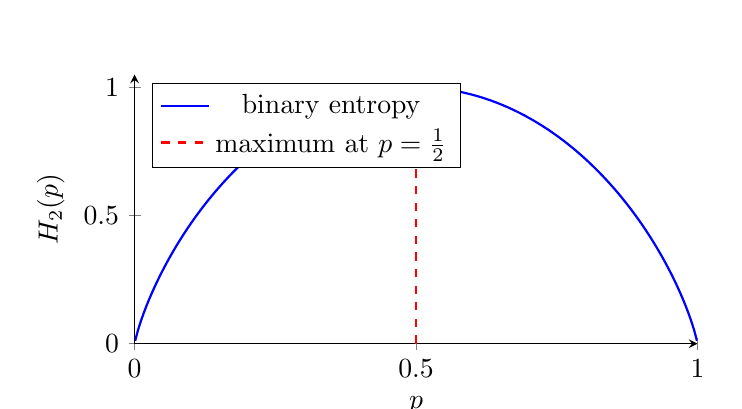
\begin{tikzpicture}
\begin{axis}[
    width=0.72\textwidth, height=5cm,
    xlabel={$p$}, ylabel={$H_2(p)$},
    domain=0.001:0.999, samples=200,
    xmin=0, xmax=1, ymin=0, ymax=1.05,
    xtick={0,0.5,1}, ytick={0,0.5,1},
    axis lines=left, legend pos=north west
]
\addplot[thick, blue] {-x*log2(x)-(1-x)*log2(1-x)};
\addlegendentry{binary entropy}
\addplot[thick, red, dashed] coordinates {(0.5,0) (0.5,1)};
\addlegendentry{maximum at $p= \frac{1}{2}$}
\end{axis}
\end{tikzpicture}
\caption{The binary entropy function $H_2(p)$ is symmetric, concave, and maximised at $p= \frac{1}{2}$.}
\label{fig:binary-entropy}
\end{figure}

\begin{example}
    Let $S = \{0,1\}$ with $p(0) = p$ and $p(1) = 1 - p$. Then
    \begin{align}
        H(p(x)) &= -p\log_2(p) - (1-p)\log_2(1-p)
    \end{align}
    The maximum entropy $H(p(x)) = 1$ is achieved when $p = \tfrac{1}{2}$, that is, when the two outcomes are equally likely.
\end{example}

\begin{example}
    \emph{Entropy of English language}: Shannon estimated the entropy of English text by having subjects predict the next letter in a sequence. He estimated that the entropy of English is approximately $1.0$ to $1.5$ bits per character. This means that despite using 26 letters (which would require $\log_2(26) \approx 4.7$ bits each if uniformly distributed), the inherent uncertainty is much lower due to the statistical structure of the language. This result has profound implications for data compression: English text can theoretically be compressed to roughly $30\%$ of its original size.
\end{example}

\begin{example}
    If $X\sim\mathrm{U}(a,b)$, then 
    \begin{align}
        H(X)=\log(b-a)
    \end{align}
    (with natural logarithms). Thus $\mathrm{U}(0,1)$ has $H=0$ nats, $\mathrm{U}(0,2)$ has $H=\log 2$ nats, and $\mathrm{U}(0,\tfrac12)$ has $H=-\log 2$ nats. Unlike discrete entropy, differential entropy may be negative; it measures spread relative to the units of $x$.
\end{example}

\begin{example}[Gaussian distribution]
    If $X\sim\mathscr{N}(\mu,\sigma^2)$, then
    \begin{align}
        H(X) &= \tfrac12\log\left(2\pi e\sigma^2\right).
    \end{align}
    For the standard normal this is $\tfrac12\log(2\pi e)\approx1.419$ nats. Increasing $\sigma$ increases the entropy by $\log\sigma$, so doubling the standard deviation adds $\log 2$ nats.
\end{example}

\begin{example}[Exponential distribution]
    If $X\sim\mathrm{Exp}(\lambda)$ with density $\lambda e^{-\lambda x}$ for $x\ge0$, then
    \begin{align}
        H(X) &= 1+\log\lambda.
    \end{align}
    For $\lambda=2$, $H=1-\log 2\approx0.307$ nats; a tighter rate concentrates the mass and lowers the entropy.
\end{example}

\begin{definition}
    A real-valued function $f$ is concave on an interval $I$ if
    \begin{align}
        f(\lambda x + (1-\lambda)y) &\geq \lambda f(x) + (1-\lambda) f(y)
    \end{align}
    for all $x, y \in I$ and every $\lambda \in [0,1]$. It is \emph{strictly concave}
    when the inequality is strict for all $x \neq y$ in $I$ and every $\lambda \in (0,1)$.
\end{definition}

\begin{example}[A concave function]
    The square root $f(x)=\sqrt{x}$ is concave on $(0,\infty)$. For $x=1$ and $y=4$,
    \begin{align}
        \frac{f(1)+f(4)}{2} &= \frac{1+2}{2}=1.5
        \leq \sqrt{2.5}\approx1.581 = f\!\left(\frac{1+4}{2}\right),
    \end{align}
    so averaging inputs gives a larger value than averaging outputs.
\end{example}

\begin{example}[Another concave function]
    The logarithm $f(x)=\log x$ is concave on $(0,\infty)$ because $f''(x)=-1/x^2<0$. For $x=1$ and $y=e^2$,
    \begin{align}
        \frac{\log 1+\log e^2}{2}=1 \leq \log\left(\frac{1+e^2}{2}\right)\approx1.434.
    \end{align}
\end{example}

\begin{example}[A concave function on a closed interval]
    The function $f(x)=x(1-x)$ is concave on $[0,1]$ since $f''(x)=-2$. Its graph is a downward parabola with maximum $1/4$ at $x=1/2$.
\end{example}

\begin{example}[A strictly concave function]
    The function $f(x)=\sin x$ is strictly concave on $[0,\pi]$ because $f''(x)=-\sin x<0$ on $(0,\pi)$. For $x=0$ and $y=\pi$,
    \begin{align}
        \frac{\sin 0+\sin\pi}{2}=0 < 1=\sin\frac{\pi}{2}.
    \end{align}
\end{example}

\begin{example}[Another strictly concave function]
    The negative quadratic $f(x)=-x^2$ is strictly concave on $\mathbb{R}$: $f''(x)=-2<0$ everywhere, and for $x\neq y$,
    \begin{align}
        \frac{f(x)+f(y)}{2} = -\frac{x^2+y^2}{2}
        < -\left(\frac{x+y}{2}\right)^2 = f\!\left(\frac{x+y}{2}\right).
    \end{align}
    The inequality is strict because $(x-y)^2>0$.
\end{example}

\begin{theorem}
    (\emph{Jensen's inequality}) Suppose $f$ is a continuous strictly concave function on the interval $I$. Suppose further that
    \begin{align}
        \sum_{i=1}^n a_i = 1
    \end{align}
    and $a_i > 0$, for $1 \leq i \leq n$. Then 
    \begin{align}
        \sum_{i=1}^n a_i f(x_i) &\leq f\bigg( \sum_{i=1}^n a_i x_i\bigg)
    \end{align}
    where $x_i \in I$, for $1 \leq i \leq n$. Further, equality occurs if and only if $x_1 = \ldots = x_n$.
\end{theorem}
\begin{proof}
    We argue by induction on $n$. For $n=2$ the statement is exactly the definition of concavity, since $a_2=1-a_1$.
    Suppose the result holds for $n-1$ weights and set $b=1-a_n>0$ and
    \begin{align}
        y = \frac{1}{b}\sum_{i=1}^{n-1} a_i x_i \in I .
    \end{align}
    The point $y$ lies in $I$ because an interval is convex. Applying the induction hypothesis to the normalised weights $a_i/b$ and then concavity to the two points $y$ and $x_n$ gives
    \begin{align}
        \sum_{i=1}^n a_i f(x_i)
        &= b\sum_{i=1}^{n-1}\frac{a_i}{b}f(x_i) + a_n f(x_n) \\
        &\leq b f(y) + a_n f(x_n) \\
        &\leq f\big( b y + a_n x_n \big)
        = f\left( \sum_{i=1}^n a_i x_i \right).
    \end{align}
    If $f$ is strictly concave, equality in the induction step forces $x_1=\cdots=x_{n-1}$, while equality in the second step forces $y=x_n$; hence all $x_i$ are equal. Conversely, equality is immediate when all $x_i$ coincide.
\end{proof}

% ref: N. Sahu - Mathematics for Machine Learning_ A Deep Dive into Algorithms (2023).pdf

\begin{definition}
    Given discrete distributions $p: S \to [0,1]$ and $q: S \to [0,1]$, the \emph{relative entropy} (\emph{information divergence}, \emph{Kullback-Leibler divergence}, $\mathrm{KL}$-divergence \index{KL-divergence} \emph{discrimination}) from $p$ to $q$ is defined as
    \begin{align}
    D_{\mathrm{KL}}(p\,\|\,q) &\defn \sum_{x \in S} p(x)\log\frac{p(x)}{q(x)}\\
    &= \underset{x\sim p}{\E}\left[\log\frac{p(x)}{q(x)}\right].
    \end{align}
    For a continuous distribution, it is given by
    \begin{align}
        D_{\mathrm{KL}}(p\,\|\,q) \defn \int p(x)\log\frac{p(x)}{q(x)} dx.
    \end{align}
    It is a measure of how much $q$ differs from $p$. Note that in general $D_{\mathrm{KL}}(p\,\|\,q) \neq D_{\mathrm{KL}}(q\,\|\,p)$.
\end{definition}

\begin{lemma}
    We have that $D_{\mathrm{KL}}(p\,\|\,q) \geq 0$ with equality if and only if $p=q$.
\end{lemma}
\begin{proof}
    Let $\mu$ denote counting measure in the discrete case and Lebesgue measure in the continuous case, so that
    \begin{align}
        D_{\mathrm{KL}}(p\,\|\,q) = \int_{\mathcal{X}} p(x)\log\frac{p(x)}{q(x)}\,d\mu(x)
    \end{align}
    specialises to a sum or an integral as appropriate. Put $S=\{x:p(x)>0\}$; where $p(x)=0$ the integrand is zero by convention. Since $-\log$ is convex, Jensen's inequality gives
    \begin{align}
        D_{\mathrm{KL}}(p\,\|\,q)
        &= -\int_S p(x)\log\frac{q(x)}{p(x)}\,d\mu(x) \\
        &\geq -\log\!\left(\int_S p(x)\frac{q(x)}{p(x)}\,d\mu(x)\right) \\
        &= -\log\!\left(\int_S q(x)\,d\mu(x)\right)
        \geq -\log 1 = 0,
    \end{align}
    because $\int_S q\,d\mu\leq\int_{\mathcal{X}} q\,d\mu=1$.

    Equality forces $\frac{q(x)}{p(x)}$ to be constant $\mu$-almost everywhere on $S$ and $\int_S q\,d\mu=1$. The latter implies $q=0$ off $S$, while the former gives $q=cp$ on $S$. Normalising $\int q\,d\mu=1$ then yields $c=1$, so $q=p$ $\mu$-almost everywhere. Conversely, $p=q$ clearly gives zero. The divergence is not symmetric: for the Bernoulli example above, $D_{\mathrm{KL}}(p\,\|\,q)\approx0.511$ while $D_{\mathrm{KL}}(q\,\|\,p)\approx0.368$.
\end{proof}

\begin{example}[Bernoulli mismatch]
    For $p=\mathscr{B}\left(\dfrac{1}{2}\right)$ and $q=\mathscr{B}(0.1)$, 
    \begin{align}
        D_{\mathrm{KL}}(p\,\|\,q) &= \tfrac12\log\tfrac{0.5}{0.1}+\tfrac12\log\tfrac{0.5}{0.9} \\
        &\approx 0.511\text{ nats},
    \end{align}
    quantifying the extra coding cost of using $q$.     Swapping the arguments gives $D_{\mathrm{KL}}(q\,\|\,p)\approx0.368\neq0.511$; the graph of $D_{\mathrm{KL}}$ as a function of $q$ is tilted and vanishes only at $q=p$.
\end{example}

\begin{example}[Gaussian mismatch]
    For $p=\mathscr{N}(0,1)$ and $q=\mathscr{N}(1,1)$,
    \begin{align}
        D_{\mathrm{KL}}(p\,\|\,q) &= \frac12\left(\frac{(0-1)^2}{1}+\frac{1}{1}-1-\log\frac{1}{1}\right) \\
        &= \frac12~\text{nats}.
    \end{align}
    The means differ by one standard deviation; the penalty is independent of the common scale.
\end{example}

The $\mathrm{KL}$-divergence has applications in the following:
\begin{enumerate}
    \item \emph{Model comparison}: KL-Divergence can be used to compare how well a model $Q$ approximates the true data distribution $P$. Smaller KL divergence indicates a better.approximation.
    \item \emph{Information Theory}: KL-Divergence is a key concept in information theory, providing a measure of how much information is lost when approximating one distribution with another.
    \item \emph{Probabilistic Modeling}: In machine learning, KL-Divergence is used in tasks like variational inference, where it quantifies the difference between the true posterior distribution and the approximating distribution.
    \item \emph{Variational Autoencoders (VAEs)}: In VAEs, KL-Divergence is used to regularize the latent space. It encourages the learned latent distribution to be similar to a known prior distribution, typically a simple Gaussian distribution.
    \item \emph{Natural Language Processing}: Supports language modeling, word embedding comparisons and topic modeling approaches such as Latent Dirichlet Allocation (LDA).
    \item \emph{Computer Vision}: Used in VAEs, GANs and recognition systems to align generated data with real world distributions.
    \item \emph{Anomaly Detection}: Identifies unusual or suspicious patterns by measuring distribution shifts, helpful in fraud detection and cybersecurity.
    \item \emph{Probabilistic Models}: Aligns learned distributions with target distributions like in Variational Autoencoders (VAEs).
    \item \emph{Reinforcement Learning}: Stabilizes policy updates in algorithms like PPO by limiting divergence from previous policies.
    \item \emph{Language Models}: Guides token probability distributions during fine-tuning and model distillation.
    \item \emph{Generative Models}: Measures how closely generated data matches real data distributions.
\end{enumerate}

\coderef{Code/information_theory.py}
\coderef{Code/entropy.ipynb}
\coderef{Code/cross_entropy.ipynb}
\coderef{Code/kl_divergence.ipynb}
\coderef{Code/bayes_rule.ipynb}

\begin{proposition}
    The $\mathrm{KL}$ divergence  is non-negative and zero iff $p=q$, but it is not symmetric. 
\end{proposition}

\begin{definition}
    The \emph{cross-entropy} between two distributions $p$ and $q$ is
    \begin{align}
        H(p,q) &\defn -\sum_x p(x)\log q(x)\\
        &=  H(p) + D_{\mathrm{KL}}(p\,\|\,q).
    \end{align}
\end{definition}
Minimising cross-entropy over $q$ is equivalent to minimising
$D_{\mathrm{KL}}(p\,\|\,q)$ because $H(p)$ does not depend on $q$. This is why cross-entropy is the standard classification loss.

\begin{example}[Binary labels]
    For $p=(1,0)$, $H(p,q)=-\log q(1)$: the loss penalises confident wrong predictions heavily and is minimised at $q(1)=1$, matching the logistic loss.
\end{example}

\begin{example}[Binary entropy relation]
    For $p=\mathrm{Bernoulli}(1/2)$ and $q=\mathrm{Bernoulli}(q_1)$, $H(p,q)=\log 2+D_{\mathrm{KL}}(p\,\|\,q)$; the curve is minimised at $q_1=1/2$, where cross-entropy equals the entropy of $p$.
\end{example}

\begin{example}[Classification]
    For a $k$-class problem with one-hot target $y$, cross-entropy reduces to $-\log q_y$, the negative log-likelihood of the true class. Minimising it is equivalent to maximum likelihood for the softmax classifier.
\end{example}

\begin{definition}
    The \emph{Jensen-Shannon divergence} between two distributions $p$ and $q$ is
    \begin{align}
        D_{\mathrm{JS}}(p\,\|\,q) = \frac{1}{2}D_{\mathrm{KL}}(p\,\|\,r) + \frac{1}{2}D_{\mathrm{KL}}(q\,\|\,r),
    \end{align}
    where $r = \frac{1}{2}(p + q)$.
\end{definition}
Some nice videos can be found \href{https://www.youtube.com/watch?v=KHVR587oW8I}{here}.

\begin{example}[Identical distributions]
    If $p=q=(0.5,0.5)$, then $r=p$ and both KL terms vanish, so $D_{\mathrm{JS}}(p\,\|\,q)=0$. In general $D_{\mathrm{JS}}=0$ only when $p=q$ almost everywhere.
\end{example}

\begin{example}[Disjoint support]
    If $p=(1,0)$ and $q=(0,1)$, then $r=(0.5,0.5)$ and
    \begin{align}
        D_{\mathrm{JS}}(p\,\|\,q) = \tfrac12\log 2+\tfrac12\log 2 = \log 2\approx0.693~\text{nats}.
    \end{align}
    This is the maximum value for binary distributions, so JS divergence is bounded, unlike KL.
\end{example}

\begin{example}[Overlapping Bernoulli laws]
    For $p=(0.9,0.1)$ and $q=(0.1,0.9)$, again $r=(0.5,0.5)$ and
    \begin{align}
        D_{\mathrm{KL}}(p\,\|\,r) = 0.9\log 1.8+0.1\log 0.2 \approx0.368,
    \end{align}
    with the same value for $D_{\mathrm{KL}}(q\,\|\,r)$ by symmetry. Hence $D_{\mathrm{JS}}(p\,\|\,q)\approx0.368$ nats, or about $0.531$ bits. Unlike KL, the JS divergence is symmetric and its square root is a metric.
\end{example}

\coderef{Code/js_divergence.ipynb}
\coderef{Code/information_theory.py}

\chapter{Introduction}
\label{ch:intro}

\begin{epigraph}
    {O, what learning is!}{William Shakespeare, Romeo and Juliet}
\end{epigraph}


\begin{epigraph}
    {Learning and intelligence are intimately related to each other. It is usually agreed that a system capable of learning deserves to be called intelligent; and conversely, a system being considered as intelligent is, among other things, usually expected to be able to learn. Learning always has to do with the self- improvement of future behaviour based on past experience.}{Sandip Sen and Gerhard Weiss, Learning in Multiagent Systems}
\end{epigraph}

What does it mean to learn? The dictionary definition is the activity or process of
gaining knowledge or skill by studying, practicing, being taught, or experiencing
something. The operational definition used in this course is Mitchell's:

\begin{epigraph}
{
A computer program is said to learn from experience $E$ with respect to some class of
tasks $T$ and performance measure $P$, if its performance at tasks in $T$, as
measured by $P$, improves with experience $E$.
}{Tom Mitchell}
\end{epigraph}

The \emph{machine-learning approach} is therefore to program an algorithm that automatically improves from data or experience, rather than to hand-code the desired behaviour. Learning problems are commonly classified along four axes.

\section{History}

\begin{table}[H]
    \centering
    \caption{A short timeline of machine learning.}
    \label{tab:ml-history}
    \begin{tabularx}{\textwidth}{@{}p{1.8cm}X@{}}
        \toprule
        Period & Milestone \\
        \midrule
        1957 & Perceptron algorithm (implemented as a circuit). \\
        1959 & Arthur Samuel's learning-based checkers program could defeat its author. \\
        1969 & Minsky and Papert's \emph{Perceptrons} exposed limitations of linear models. \\
        1980s & Connectionist psychologists explored neural models of cognition. \\
        1984 & Leslie Valiant formalised learning as PAC learning. \\
        1986 & Backpropagation (re)discovered by Geoffrey Hinton and colleagues. \\
        1988 & Judea Pearl's \emph{Probabilistic Reasoning in Intelligent Systems} introduced Bayesian networks. \\
        1990s & The ``AI Winter'': pessimism and low funding. \\
        1990s & A golden age for ML research: Markov chain Monte Carlo, variational inference, kernels and support vector machines, boosting, and convolutional networks. \\
        2000s & Applied AI fields (vision, NLP, etc.) adopted ML. \\
        2010s & Deep learning. \\
        2010--2012 & Neural networks broke previous records in speech-to-text and object recognition, and industry adoption accelerated. \\
        2016 & AlphaGo defeated the human Go champion. \\
        2017--2026 & Transformers (2017) enabled large language models; AlphaFold~2 (2020) advanced protein structure prediction; diffusion models (2020--2024) transformed image generation; ChatGPT (2022) and multimodal reasoning models (2024--2026) brought generative AI into widespread use. \\
        \bottomrule
    \end{tabularx}
\end{table}

\section{ML workflow}

We formulate machine learning as combinations of three components:
\begin{enumerate}
    \item \emph{Data}: Collections of individual data points that are characterized by features.
    \item \emph{Model}: a model or hypothesis space that consists of computationally feasible hypothesis.
    \item \emph{Loss function}: a function that measures the quality of a hypothesis map.
\end{enumerate}

% \item  Should I use ML on this problem?
    % \item \begin{enumerate}
    %     \item Is there a pattern to detect?
    %     \item Can I solve it analytically?
    %     \item Do I have data?
    % \end{enumerate}

Once we have decided a ML strategy for the problem at hand. Here is the sketch of the workflow:
\begin{enumerate}
    \item Gather and organize data.
    \item Load and inspect the data.
    \item Preprocessing, cleaning, visualizing.
    \item Establishing a baseline.
    \item Standardize the features.
    \item Choosing a model, loss, regularization.
    \item Optimization (could be simple, could be a Phd.).
    \item Hyperparameter search.
    \item Analyze performance and mistakes, and iterate back.
\end{enumerate}

\section{Supervised versus unsupervised}

\begin{enumerate}
    \item \emph{Supervised learning}: build a model that predicts an output from
    inputs using labelled examples.
    \begin{enumerate}
        \item \emph{Classification}: the output is qualitative (categorical).
        \begin{example}
            Predict whether a credit-card transaction is fraudulent.
        \end{example}
        \item \emph{Regression}: the output is quantitative (continuous or ordered).
        \begin{example}
            Predict the value of a stock tomorrow.
        \end{example}
    \end{enumerate}
    \item \emph{Unsupervised learning}: learn structure from data without a supervised
    output signal.
    \begin{enumerate}
        \item \emph{Clustering}: partition observations into groups that share common
        characteristics.
        \item \emph{Dimensionality reduction}: construct new features from the original
        inputs that retain important information.
        \item \emph{Density estimation}: model the probability distribution of the data.
    \end{enumerate}
    \item \emph{Reinforcement learning}: learn a policy for selecting actions based on
    rewards received from an environment.
\end{enumerate}

Two important intermediate settings are \emph{semi-supervised learning} (a small
labelled set together with a large unlabelled set) and \emph{self-supervised learning}
(labels are generated from the data itself, as in masked-language modelling).

\section{Active versus passive learners}

A \emph{passive} learner receives data without influencing which examples are
collected. An \emph{active} learner can request labels for particular examples, which
is valuable when labelling is expensive. The central question is which query is most
informative.

\section{Online versus batch learning}

In \emph{batch} learning the entire training set is available before training starts.
In \emph{online} learning examples arrive sequentially and the model is updated after
each one. Online methods are natural when the data distribution changes over time,
but they require care with learning rates, stability, and catastrophic forgetting.

\section{Helpfulness of the teacher}

The teacher may provide only labels, or may additionally provide explanations,
demonstrations, constraints, or rewards. The more helpful the teacher, the less data
and computation are usually required, but the harder it is to specify the teaching
signal.

\section{Inductive bias and the no-free-lunch theorem}

Every learner must make assumptions that go beyond the training data; these
assumptions are its \emph{inductive bias}. A convolutional network assumes that
nearby pixels are related and that patterns are translation-equivariant. A decision
tree assumes that axis-aligned splits are useful. The no-free-lunch theorem makes
this unavoidable:

\begin{theorem}[No free lunch, Wolpert 1996]
Averaged over all possible target functions, every learning algorithm has the same
expected off-training-set performance.
\end{theorem}

The theorem does not say that all algorithms are equally good in practice. Real problems are not uniformly distributed, and a good inductive bias matches the structure of the problem. Model choice is therefore the art of choosing assumptions that are appropriate for the data at hand.

\chapter{Supervised Learning}
\label{ch:supervised}

This chapter introduces the supervised-learning problem and the language used
throughout the rest of the notes. We first formalise labelled data, features and
targets, and illustrate the range of tasks with examples spanning regression,
binary classification, multiclass classification and structured output. We then
define loss functions, risk and empirical risk, which turn ``good prediction''
into an optimisation problem, and state the empirical risk minimisation
principle. The first learning algorithm we study is \texorpdfstring{$k$}{k}-nearest
neighbours: simple, nonparametric, and a useful baseline. The remainder of the
chapter asks how performance should be measured: training/validation/test splits,
cross-validation, error metrics, model flexibility, the bias--variance
decomposition, and the curse of dimensionality. Later chapters instantiate the
same framework with linear models, trees, kernels and neural networks.

\section{The supervised-learning problem}

Let $X \subseteq \mathbb{R}^{d}$ be the input space (predictors, independent variables, features) and $Y \subseteq \mathbb{R}$\footnote{In general, the output space can be in $\mathbb{R}^k$ for some $k \geq 1$.} the output space (response, dependent variable). We observe
the \emph{data set} of labelled pairs
\begin{align}
    D = \bigg\{ (\mathbf{x}^{(1)}, y_1), (\mathbf{x}^{(2)}, y_2), \ldots, (\mathbf{x}^{(n)}, y_n) \bigg\} \subseteq X \times Y,
\end{align}
drawn from an unknown joint distribution $\mathscr{D}$ over $X \times Y$. The goal is to learn a function
$f : X \to Y$ that predicts $y$ from $\mathbf{x}$ and
generalises to new observations.  The classical statistical model is
\begin{align}
    y = f(\mathbf{x}) + \varepsilon,
\end{align}
where $f$ is the systematic part and $\varepsilon$ is irreducible noise with average $\E[\varepsilon]=0$. Even with a perfect estimate of $f$, the noise limits how
accurate any prediction can be.

In supervised learning, the input is represented by a vector
$\mathbf{x} \in \R^d$. Each coordinate $x_i$ is a \emph{feature}\index{feature}, a numerical value describing a characteristic of the input. Images, text, audio, and waveforms can all be represented this way (images as pixel vectors, text as token counts or embeddings, audio as frames). Vector representations are convenient because we can apply linear algebra. The output is represented by a number $t \in \R$ in regression, or by an element of a discrete set in classification.

\innote{Prediction versus inference}{%
Predicting the response $y$ given inputs $\mathbf{x}$ is \emph{prediction}.
Understanding how the response depends on individual predictors $x_i$ is
\emph{inference}. Inference often requires an interpretable model rather than a
black box.}

\section{Examples of supervised learning}

\begin{example}[\emph{Age prediction}]
Given a headshot, predict the person's age. Input: an image; output: a real number.
\begin{center}
\begin{tikzpicture}[node distance=0.9cm, >=Latex,
    every node/.style={draw, rounded corners, align=center, font=\small}]
    \node (img) {headshot\\$64\times64$ pixels};
    \node[right=of img] (vec) {features\\$\mathbf{x}\in\R^{4096}$};
    \node[right=of vec] (pred) {predictor\\$f$};
    \node[right=of pred] (out) {age\\$\hat y\in\R$};
    \draw[->] (img) -- (vec);
    \draw[->] (vec) -- (pred);
    \draw[->] (pred) -- (out);
\end{tikzpicture}
\end{center}
Representative training examples $(\mathbf{x}^{(i)},y_i)$, summarised by two
features extracted from each image, are:
\begin{center}
\begin{tabular}{@{}lccc@{}}
\toprule
Image & Mean intensity & Eye spacing (px) & Age (years) \\
\midrule
A & $0.62$ & $28$ & $24$ \\
B & $0.55$ & $31$ & $47$ \\
C & $0.68$ & $26$ & $19$ \\
\bottomrule
\end{tabular}
\end{center}
\end{example}

\begin{example}[\emph{Image captioning}]
Given an image, produce a description. Input: an image; output: a sequence of words.
\begin{center}
\begin{tikzpicture}[node distance=0.9cm, >=Latex,
    every node/.style={draw, rounded corners, align=center, font=\small}]
    \node (img) {image};
    \node[right=of img] (vec) {visual features\\$\mathbf{z}\in\R^{512}$};
    \node[right=of vec] (pred) {sequence model\\$g$};
    \node[right=of pred] (out) {caption\\$\hat y_{1:T}$};
    \draw[->] (img) -- (vec);
    \draw[->] (vec) -- (pred);
    \draw[->] (pred) -- (out);
\end{tikzpicture}
\end{center}
\begin{center}
\begin{tabularx}{\textwidth}{@{}lXX@{}}
\toprule
Image & Detected objects & Target caption \\
\midrule
A & dog, grass & ``A dog runs on the grass.'' \\
B & bus, street & ``A bus drives down a street.'' \\
C & person, kite & ``A person flies a kite.'' \\
\bottomrule
\end{tabularx}
\end{center}
Here the output space $Y$ consists of variable-length sequences rather than a
single number.
\end{example}

\begin{example}[\emph{Exam grade}]
Given assignment and participation records, predict the final exam grade.
\begin{center}
\begin{tikzpicture}[node distance=0.9cm, >=Latex,
    every node/.style={draw, rounded corners, align=center, font=\small}]
    \node (rec) {student records};
    \node[right=of rec] (vec) {features\\assignment, participation};
    \node[right=of vec] (pred) {regressor\\$f$};
    \node[right=of pred] (out) {exam grade\\$\hat y\in\R$};
    \draw[->] (rec) -- (vec);
    \draw[->] (vec) -- (pred);
    \draw[->] (pred) -- (out);
\end{tikzpicture}
\end{center}
\begin{center}
\begin{tabular}{@{}lccc@{}}
\toprule
Student & Assignments & Participation & Exam grade \\
\midrule
1 & $88\%$ & $9/10$ & $82$ \\
2 & $61\%$ & $5/10$ & $58$ \\
3 & $95\%$ & $10/10$ & $91$ \\
\bottomrule
\end{tabular}
\end{center}
This is a regression problem: the target is a real-valued score.
\end{example}

\begin{example}[\emph{Email spam detection}]
Given an email, predict whether it is spam. Input: text and metadata; output: spam/not-spam.
\begin{center}
\begin{tikzpicture}[node distance=0.9cm, >=Latex,
    every node/.style={draw, rounded corners, align=center, font=\small}]
    \node (mail) {email};
    \node[right=of mail] (vec) {word counts\\$+$ metadata};
    \node[right=of vec] (pred) {classifier\\$f$};
    \node[right=of pred] (out) {label\\$\hat y\in\{0,1\}$};
    \draw[->] (mail) -- (vec);
    \draw[->] (vec) -- (pred);
    \draw[->] (pred) -- (out);
\end{tikzpicture}
\end{center}
\begin{center}
\begin{tabular}{@{}lccc@{}}
\toprule
Email & Count of ``free'' & Number of links & Label \\
\midrule
A & $4$ & $12$ & spam \\
B & $0$ & $1$ & not spam \\
C & $2$ & $7$ & spam \\
\bottomrule
\end{tabular}
\end{center}
\end{example}

\begin{example}[\emph{Iris classification}]
Classify iris flowers into species from petal and sepal measurements.
\begin{center}
\begin{tikzpicture}[node distance=0.9cm, >=Latex,
    every node/.style={draw, rounded corners, align=center, font=\small}]
    \node (flower) {flower};
    \node[right=of flower] (vec) {measurements\\$\mathbf{x}\in\R^4$};
    \node[right=of vec] (pred) {classifier\\$f$};
    \node[right=of pred] (out) {species\\$\hat y\in\{1,2,3\}$};
    \draw[->] (flower) -- (vec);
    \draw[->] (vec) -- (pred);
    \draw[->] (pred) -- (out);
\end{tikzpicture}
\end{center}
\begin{center}
\begin{tabular}{@{}ccccc@{}}
\toprule
Sepal length & Sepal width & Petal length & Petal width & Species \\
\midrule
$5.1$ & $3.5$ & $1.4$ & $0.2$ & setosa \\
$6.4$ & $3.2$ & $4.5$ & $1.5$ & versicolor \\
$6.3$ & $3.3$ & $6.0$ & $2.5$ & virginica \\
\bottomrule
\end{tabular}
\end{center}
All measurements are in centimetres; this is a three-class problem.
\end{example}

\begin{example}[\emph{Sentiment analysis}]
Given a piece of text, predict positive, negative, or neutral sentiment.
\begin{center}
\begin{tikzpicture}[node distance=0.9cm, >=Latex,
    every node/.style={draw, rounded corners, align=center, font=\small}]
    \node (text) {text};
    \node[right=of text] (vec) {features\\token counts};
    \node[right=of vec] (pred) {classifier\\$f$};
    \node[right=of pred] (out) {sentiment\\$\hat y$};
    \draw[->] (text) -- (vec);
    \draw[->] (vec) -- (pred);
    \draw[->] (pred) -- (out);
\end{tikzpicture}
\end{center}
\begin{center}
\begin{tabularx}{\textwidth}{@{}lXX@{}}
\toprule
Text snippet & Informative tokens & Label \\
\midrule
``The film was delightful.'' & delightful & positive \\
``It was dull and too long.'' & dull, long & negative \\
``The film was released today.'' & released & neutral \\
\bottomrule
\end{tabularx}
\end{center}
\end{example}

\begin{example}[\emph{Handwritten digits}]
Given an image of a digit, predict which digit it is.
\begin{center}
\begin{tikzpicture}[node distance=0.9cm, >=Latex,
    every node/.style={draw, rounded corners, align=center, font=\small}]
    \node (img) {digit image\\$28\times28$};
    \node[right=of img] (vec) {pixels\\$\mathbf{x}\in\R^{784}$};
    \node[right=of vec] (pred) {classifier\\$f$};
    \node[right=of pred] (out) {digit\\$\hat y\in\{0,\ldots,9\}$};
    \draw[->] (img) -- (vec);
    \draw[->] (vec) -- (pred);
    \draw[->] (pred) -- (out);
\end{tikzpicture}
\end{center}
\begin{center}
\begin{tabular}{@{}lcc@{}}
\toprule
Image & Centre-pixel intensity & True digit \\
\midrule
A & $0.00$ & $0$ \\
B & $0.94$ & $1$ \\
C & $0.76$ & $7$ \\
\bottomrule
\end{tabular}
\end{center}
This is a ten-class classification problem.
\end{example}

\section{Loss functions, risk, and empirical risk}

To say what a \emph{good} prediction is, we need a loss function $\ell(y,\hat{y})$. Common choices are squared error for regression, 
\begin{align}
    \ell(y,\hat{y})=(y-\hat{y})^2,
\end{align}
and the zero-one loss for classification, 
\begin{align}
    \ell(y,\hat{y})&=\begin{cases}
        1, &\text{if $y \neq \hat{y}$},\\
        0, &\text{otherwise}.
    \end{cases}
\end{align}
\begin{definition}
The \emph{risk} of a predictor $f$ is the expected loss under the data distribution:
\begin{align}
    \risk(f) \defn \underset{(\mathbf{x},y)\sim\mathscr{D}}{\E}[\ell(y,f(\mathbf{x}))].
\end{align}
The \emph{empirical risk} is defined as 
\begin{align}
    \widehat{\risk}_n(f) \defn \frac{1}{n}\sum_{i=1}^n \ell(y_i, f(\mathbf{x}^{(i)})).
\end{align}
\end{definition}
\begin{example}[Squared error]
    For squared-error loss and a linear predictor 
    \begin{align}
        f(\mathbf{x})=\mathbf{x}^\top\boldsymbol{\beta},
    \end{align}
    the risk 
    \begin{align}
        \risk(f)=\E[(y-f(\mathbf{x}))^2]
    \end{align}
    is the mean squared error; its empirical counterpart is 
    \begin{align}
        \widehat\risk_n(f)=\frac1n\sum_i(y_i-f(\mathbf{x}^{(i)}))^2.
    \end{align}
    For example, let $n=3$, $f(x)=2x+1$ and take the data below.
    \begin{center}
    \begin{tabular}{@{}cccc@{}}
        \toprule
        $x_i$ & $y_i$ & $f(x_i)$ & $(y_i-f(x_i))^2$ \\
        \midrule
        $1$ & $4$ & $3$ & $1$ \\
        $2$ & $6$ & $5$ & $1$ \\
        $3$ & $7$ & $7$ & $0$ \\
        \bottomrule
    \end{tabular}
    \end{center}
    The squared errors sum to $2$, so
    $\widehat\risk_3(f)=2/3\approx0.667$. The empirical risk is just the
    average of the last column; the true risk $\risk(f)$ replaces that average
    with an expectation over the unknown distribution $\mathscr{D}$.
\end{example}

\begin{example}[Zero-one loss]
    For zero-one loss, 
    \begin{align}
        \risk(f)=\Pr(y\neq f(\mathbf{x}))
    \end{align}
    is the misclassification probability, while $\hat\risk_n(f)$ is the fraction of errors on the training set.
    \begin{center}
    \begin{tabular}{@{}cccc@{}}
        \toprule
        $i$ & $y_i$ & $f(\mathbf{x}^{(i)})$ & $\mathbf{1}_{\{y_i\neq f(\mathbf{x}^{(i)})\}}$ \\
        \midrule
        $1$ & $0$ & $0$ & $0$ \\
        $2$ & $1$ & $1$ & $0$ \\
        $3$ & $0$ & $1$ & $1$ \\
        $4$ & $1$ & $1$ & $0$ \\
        \bottomrule
    \end{tabular}
    \end{center}
    On these $n=4$ examples there is one mistake, so
    $\hat\risk_4(f)=1/4=0.25$: the empirical misclassification rate. If these
    data are representative of $\mathscr{D}$, this estimates
    $\Pr(y\neq f(\mathbf{x}))$.
\end{example}

\begin{example}[Irreducible noise]
    If 
    \begin{align}
        y=f^*(\mathbf{x})+\varepsilon
    \end{align}
    with $\E[\varepsilon]=0$ and $\Var(\varepsilon)=\sigma^2$, then even the true predictor has risk $\risk(f^*)=\sigma^2$: the irreducible noise floor.
    Take $f^*(x)=2x$ and let $\varepsilon$ be $-1$ or $+1$ with equal
    probability, so $\sigma^2=1$. One realisation of $n=4$ observations is:
    \begin{center}
    \begin{tabular}{@{}ccccc@{}}
        \toprule
        $x_i$ & $f^*(x_i)$ & $\varepsilon_i$ & $y_i$ & $(y_i-f^*(x_i))^2$ \\
        \midrule
        $1$ & $2$ & $-1$ & $1$ & $1$ \\
        $2$ & $4$ & $+1$ & $5$ & $1$ \\
        $3$ & $6$ & $-1$ & $5$ & $1$ \\
        $4$ & $8$ & $+1$ & $9$ & $1$ \\
        \bottomrule
    \end{tabular}
    \end{center}
    Even with the correct predictor, every squared error equals $\sigma^2=1$ and
    $\hat\risk_4(f^*)=1$. More data cannot remove this floor; it only helps us
    estimate $f^*$ more accurately.
\end{example}

\begin{principle}
The \emph{empirical risk minimisation} (ERM) principle states that we should choose the predictor that minimises the empirical risk.
\end{principle}
Much of learning theory (Chapter~\ref{ch:slt}) studies when small empirical risk implies small true risk.

\section{\texorpdfstring{$k$}{k}-nearest neighbours}

The $k$-nearest-neighbour ($k$-NN) classifier is one of the simplest learners. It stores the training data and, for a new point $\mathbf{x}$, finds the $k$ closest training points and predicts the most common label among them (for regression, the average target). It is a \emph{non-parametric}, \emph{instance-based} method. 

% Three practical issues dominate:
% \begin{enumerate}
%     \item \textbf{Distance metric.} Euclidean distance is standard, but features must be scaled first. For high-dimensional data, cosine or learned distances may be better.
%     \item \textbf{Choice of $k$.} Small $k$ gives a flexible, low-bias, high-variance classifier; large $k$ gives a smooth, high-bias, low-variance classifier.
%     \item \textbf{Computational cost.} Prediction requires comparing the query with all stored examples unless a spatial index is used.
% \end{enumerate}
% The bias-variance trade-off in $k$ is a concrete illustration of the general
% trade-off discussed below.

\begin{problem}
   Let $X$ be the data space, where we can think of $X$ as a set of points in Euclidean space\footnote{or with any other metric space}, along with a labelling function $f: X \longrightarrow Y$, where $Y$ is the set of labels. We are given some training data $\hat{f} \subseteq f$, where each point $(\hat{\mathbf{x}}, \hat{y}) \in \hat{f}$ informs us that the point $\hat{\mathbf{x}}$ has label $\hat{y}$. Given a point $\mathbf{x} \in X$, we want to (predict its label i.e.) find the closest point $\hat{\mathbf{x}} \in \hat{X}$ such that the distance $d(\mathbf{x}, \hat{\mathbf{x}})$ is minimised. That is, find 
   \begin{align}
        \hat{\mathbf{x}} = \arg\min_{\hat{\mathbf{x}} \in \hat{X}} d(\mathbf{x}, \hat{\mathbf{x}})
   \end{align}
   and output $\hat{y} = f(\hat{\mathbf{x}})$.
\end{problem}

The problem can be visualized using a \emph{Voronoi diagram}: a partition of the input space into regions, one around each training point, such that every location in a given region is closer to its associated training point than to any other.

\begin{example}[Voronoi diagram for six training points]
    Figure~\ref{fig:voronoi} shows six labelled training points and the Voronoi
    partition they induce. The cells of the three blue points (class $0$) and the
    three red points (class $1$) tile the plane. Inside a cell, the corresponding
    training point is the nearest neighbour, so the $1$-NN classifier predicts the
    label of that point everywhere in the cell.
\end{example}

\begin{figure}[H]
    \centering
    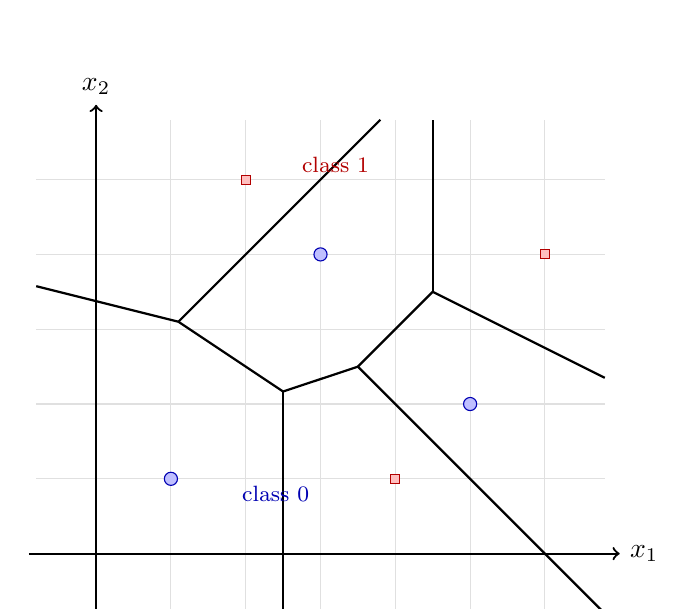
\begin{tikzpicture}[scale=0.95]
        % Background grid and axes.
        \draw[black!12, thin, step=1] (-0.8,-0.8) grid (6.8,5.8);
        \draw[->, thick] (-0.9,0) -- (7.0,0) node[right] {$x_1$};
        \draw[->, thick] (0,-0.9) -- (0,6.0) node[above] {$x_2$};

        % Voronoi edges, clipped to the plotting rectangle.
        \draw[black, thick] (1.1,3.1) -- (2.5,2.1667);
        \draw[black, thick] (1.1,3.1) -- (3.8,5.8);
        \draw[black, thick] (1.1,3.1) -- (-0.8,3.575);
        \draw[black, thick] (2.5,2.1667) -- (2.5,-0.8);
        \draw[black, thick] (2.5,2.1667) -- (3.5,2.5);
        \draw[black, thick] (3.5,2.5) -- (4.5,3.5);
        \draw[black, thick] (4.5,3.5) -- (4.5,5.8);
        \draw[black, thick] (4.5,3.5) -- (6.8,2.35);
        \draw[black, thick] (3.5,2.5) -- (6.8,-0.8);

        % Training points of class 0.
        \filldraw[blue!70!black, fill=blue!25] (1,1) circle (2.5pt);
        \filldraw[blue!70!black, fill=blue!25] (3,4) circle (2.5pt);
        \filldraw[blue!70!black, fill=blue!25] (5,2) circle (2.5pt);

        % Training points of class 1.
        \filldraw[red!70!black, fill=red!25] (1.94,4.94) rectangle (2.06,5.06);
        \filldraw[red!70!black, fill=red!25] (3.94,0.94) rectangle (4.06,1.06);
        \filldraw[red!70!black, fill=red!25] (5.94,3.94) rectangle (6.06,4.06);

        \node[font=\footnotesize, blue!70!black] at (2.4,0.8) {class $0$};
        \node[font=\footnotesize, red!70!black] at (3.2,5.2) {class $1$};
    \end{tikzpicture}
    \caption{Voronoi diagram for six training points. Each cell contains the points
    that are closer to its associated training point than to any other training
    point.}
    \label{fig:voronoi}
\end{figure}

\begin{example}[Classifying a new point by $k$-NN]
    Take the six training points of Figure~\ref{fig:voronoi} and query
    $\mathbf{x}=(3.2,2.5)$. Its distances to the training points, in increasing
    order, are:
    \begin{center}
    \begin{tabular}{@{}lccc@{}}
        \toprule
        Training point & Label & Distance & Rank \\
        \midrule
        $(3,4)$ & $0$ & $1.513$ & $1$ \\
        $(4,1)$ & $1$ & $1.700$ & $2$ \\
        $(5,2)$ & $0$ & $1.868$ & $3$ \\
        $(1,1)$ & $0$ & $2.663$ & $4$ \\
        $(2,5)$ & $1$ & $2.773$ & $5$ \\
        $(6,4)$ & $1$ & $3.176$ & $6$ \\
        \bottomrule
    \end{tabular}
    \end{center}
    For $k=1$ the prediction is the label of $(3,4)$, namely $0$. For $k=3$ the
    labels of the three nearest points are $0,1,0$, whose majority is again $0$.
    The query point lies in the Voronoi cell of $(3,4)$.
\end{example}

The \emph{decision boundary} is the boundary between regions of input space assigned to different categories. 

\begin{example}[Decision boundary of a $1$-NN classifier]
    In the six-point example, the decision boundary of the $1$-NN rule is the
    union of those Voronoi edges that separate training points of different
    labels. These edges are drawn as thick lines in
    Figure~\ref{fig:knn-boundary}. Crossing one of them changes the nearest
    training point from a class-$0$ point to a class-$1$ point (or vice versa),
    so the predicted label changes.
\end{example}

\begin{figure}[H]
    \centering
    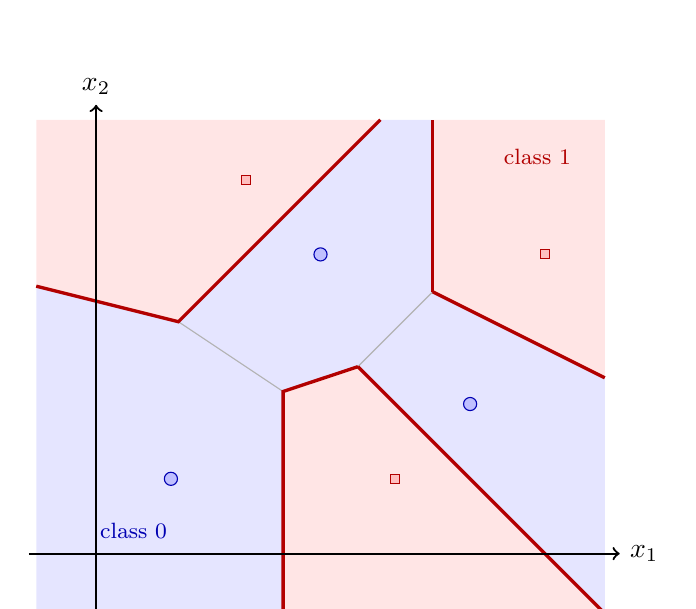
\begin{tikzpicture}[scale=0.95]
        % Shade the decision regions according to the label of the nearest point.
        \fill[blue!10] (-0.8,-0.8) -- (2.5,-0.8) -- (2.5,2.1667) --
            (1.1,3.1) -- (-0.8,3.575) -- cycle;
        \fill[blue!10] (1.1,3.1) -- (2.5,2.1667) -- (3.5,2.5) --
            (4.5,3.5) -- (4.5,5.8) -- (3.8,5.8) -- cycle;
        \fill[blue!10] (3.5,2.5) -- (4.5,3.5) -- (6.8,2.35) --
            (6.8,-0.8) -- cycle;
        \fill[red!10] (-0.8,3.575) -- (1.1,3.1) -- (3.8,5.8) --
            (-0.8,5.8) -- cycle;
        \fill[red!10] (2.5,-0.8) -- (2.5,2.1667) -- (3.5,2.5) --
            (6.8,-0.8) -- cycle;
        \fill[red!10] (4.5,3.5) -- (4.5,5.8) -- (6.8,5.8) --
            (6.8,2.35) -- cycle;

        % Voronoi edges inside a class are drawn faintly.
        \draw[black!30, thin] (1.1,3.1) -- (2.5,2.1667);
        \draw[black!30, thin] (3.5,2.5) -- (4.5,3.5);

        % Edges that separate the two classes.
        \draw[red!70!black, very thick] (-0.8,3.575) -- (1.1,3.1) -- (3.8,5.8);
        \draw[red!70!black, very thick] (2.5,-0.8) -- (2.5,2.1667) -- (3.5,2.5);
        \draw[red!70!black, very thick] (3.5,2.5) -- (6.8,-0.8);
        \draw[red!70!black, very thick] (4.5,3.5) -- (4.5,5.8);
        \draw[red!70!black, very thick] (4.5,3.5) -- (6.8,2.35);

        % Training points.
        \filldraw[blue!70!black, fill=blue!25] (1,1) circle (2.5pt);
        \filldraw[blue!70!black, fill=blue!25] (3,4) circle (2.5pt);
        \filldraw[blue!70!black, fill=blue!25] (5,2) circle (2.5pt);
        \filldraw[red!70!black, fill=red!25] (1.94,4.94) rectangle (2.06,5.06);
        \filldraw[red!70!black, fill=red!25] (3.94,0.94) rectangle (4.06,1.06);
        \filldraw[red!70!black, fill=red!25] (5.94,3.94) rectangle (6.06,4.06);

        \draw[->, thick] (-0.9,0) -- (7.0,0) node[right] {$x_1$};
        \draw[->, thick] (0,-0.9) -- (0,6.0) node[above] {$x_2$};
        \node[font=\footnotesize, blue!70!black] at (0.5,0.3) {class $0$};
        \node[font=\footnotesize, red!70!black] at (5.9,5.3) {class $1$};
    \end{tikzpicture}
    \caption{Decision boundary of the $1$-NN classifier for the data of
    Figure~\ref{fig:voronoi}. The thick segments separate the class-$0$ and
    class-$1$ decision regions; the faint segments are Voronoi edges between
    points of the same class.}
    \label{fig:knn-boundary}
\end{figure}

\begin{example}[A linear decision boundary]
    A logistic-regression classifier with $\mathbf{w}=(1,1)^\top$ and $b=-6$
    predicts class $1$ when $x_1+x_2>6$ and class $0$ otherwise. Its decision
    boundary is the straight line $x_1+x_2=6$. For instance, the score at
    $(2,2)$ is $2+2-6=-2$, so the predicted label is $0$, while the score at
    $(3,4)$ is $3+4-6=1$, so the predicted label is $1$. Unlike the piecewise
    linear $1$-NN boundary in Figure~\ref{fig:knn-boundary}, this boundary is a
    single line.
\end{example}

\begin{problem}
    Find $k$-closest point
    \begin{align}
        \hat{\mathbf{x}}_1 &= \arg\min_{\hat{\mathbf{x}} \in \hat{X}} d(\mathbf{x}, \hat{\mathbf{x}}) \\
    \hat{\mathbf{x}}_2 &= \arg\min_{\hat{\mathbf{x}} \in \hat{X} \backslash \{\hat{\mathbf{x}}_1\}} d(\mathbf{x}, \hat{\mathbf{x}}) \\
                \vdots \\
    \hat{\mathbf{x}}_k &= \arg\min_{\hat{\mathbf{x}} \in \hat{X} \backslash \{\hat{\mathbf{x}}_1, \ldots, \hat{\mathbf{x}}_{k-1}\}} d(\mathbf{x}, \hat{\mathbf{x}})
   \end{align}
   and then let $\hat{t}_i = f(\hat{\mathbf{x}}_i)$ for $i = 1, \ldots, k$. Let $\hat{t}$ be the mode of these values.
\end{problem}

\begin{example}[Two moons]
    The two-moons\index{two moons} dataset is a classic synthetic benchmark in machine learning and data science consisting of two interleaving half-circle shapes in a 2D plane. Each moon is one class: the points of one moon form a crescent that wraps around the other, so the two classes cannot be separated by a straight line. This makes it a good test for classifiers that can learn non-linear decision boundaries, such as kernel methods or neural networks.
    A few representative points are:
    \begin{center}
    \begin{tabular}{@{}lccc@{}}
        \toprule
        Point & $x_1$ & $x_2$ & Class \\
        \midrule
        A & $1.00$ & $0.00$ & $0$ \\
        B & $0.00$ & $1.00$ & $0$ \\
        C & $-1.00$ & $0.00$ & $0$ \\
        D & $0.00$ & $0.50$ & $1$ \\
        E & $1.00$ & $-0.50$ & $1$ \\
        F & $2.00$ & $0.50$ & $1$ \\
        \bottomrule
    \end{tabular}
    \end{center}
    Class $0$ lies on the upper semicircle of radius $1$ centred at the origin;
    class $1$ lies on the lower semicircle of radius $1$ centred at $(1,0.5)$.
    No straight line separates the two classes.
\end{example}

\begin{example}[Image Classification Datasets: MNIST]
    MNIST is a classic handwritten-digit dataset: 10 classes (digits 0 to 9), each image is $28\times28$ grayscale, and the standard split is 60k training images and 10k test images (often repartitioned as 50k train, 10k validation, and 10k test). Despite its small size by modern standards, MNIST remains a common first benchmark because it is easy to load, quick to train on, and illustrates the whole image-classification pipeline.
    Each example is a pair $(\mathbf{x},y)$ with $\mathbf{x}\in[0,1]^{784}$ and
    $y\in\{0,\ldots,9\}$. Four pixel values from three typical images are:
    \begin{center}
    \begin{tabular}{@{}lccccc@{}}
        \toprule
        Image & $x_{13,13}$ & $x_{13,14}$ & $x_{14,13}$ & $x_{14,14}$ & Label \\
        \midrule
        A & $0.00$ & $0.21$ & $0.00$ & $0.00$ & $0$ \\
        B & $0.94$ & $0.88$ & $0.00$ & $0.00$ & $1$ \\
        C & $0.76$ & $0.81$ & $0.12$ & $0.03$ & $7$ \\
        \bottomrule
    \end{tabular}
    \end{center}
    A digit $0$ is dark around the boundary and light in the centre, while $1$
    has a bright vertical stroke near the middle.
\end{example}

\begin{example}[Image Classification Datasets: ImageNet]
    ImageNet is a large-scale image-classification benchmark with 1000 classes. The standard version (ILSVRC) contains roughly 1.3M training images (about 1.3K per class), 50K validation images (50 per class), and 100K test images (100 per class). Its size and diversity made it the key driver of the deep-learning revolution in computer vision beginning around 2012.
    A single validation example has the following structure:
    \begin{center}
    \begin{tabular}{@{}llll@{}}
        \toprule
        Image id & Input $\mathbf{x}$ & True class $y$ & Prediction $\hat y$ \\
        \midrule
        A & $224\times224\times3$ & \texttt{tabby\ cat} & \texttt{tabby\ cat} \\
        B & $224\times224\times3$ & \texttt{sports\ car} & \texttt{sports\ car} \\
        C & $224\times224\times3$ & \texttt{banana} & \texttt{orange} \\
        \bottomrule
    \end{tabular}
    \end{center}
    Under top-1 accuracy, images A and B score $1$ and image C scores $0$;
    top-5 accuracy also counts a prediction if the true class appears among the
    five most likely classes.
\end{example}

\begin{example}[IRIS]
    The IRIS dataset is one of the most famous small datasets in statistics and machine learning. It contains 150 measurements of iris flowers: 50 from each of three species (setosa, versicolor, virginica). For each flower it records four features---sepal length, sepal width, petal length, and petal width---in centimetres. It is often used to teach classification, clustering, and data visualisation because it is small, easy to understand, and exhibits clear structure.
    A representative training set is:
    \begin{center}
    \begin{tabular}{@{}ccccc@{}}
        \toprule
        Sepal length & Sepal width & Petal length & Petal width & Species \\
        \midrule
        $5.1$ & $3.5$ & $1.4$ & $0.2$ & setosa \\
        $6.4$ & $3.2$ & $4.5$ & $1.5$ & versicolor \\
        $6.3$ & $3.3$ & $6.0$ & $2.5$ & virginica \\
        \bottomrule
    \end{tabular}
    \end{center}
    Setosa has short, narrow petals and is linearly separable; versicolor and
    virginica overlap, so a perfect classifier is impossible.
\end{example}


\section{}

\section{Assessing model performance}

We want to know how well predictions will work on previously unseen data. The ability
to generalise is what makes a learned model useful. The available data are usually
split into three parts:
\begin{enumerate}
    \item \emph{Training data}: used to fit the model parameters.
    \item \emph{Validation data}: used to tune hyperparameters and select the best
    model.
    \item \emph{Test data}: used once, at the end, to evaluate the final model. It is
    not available to the algorithm during any part of the learning process.
\end{enumerate}
The test set must never influence training or hyperparameter choices; otherwise the
reported error is biased downward. Chapter~\ref{ch:cv} develops cross-validation and
nested procedures for using data efficiently.

\section{Model flexibility, underfitting, and overfitting}

\emph{Model flexibility} (also called model \emph{capacity}) is a measure of how rich
a family of functions the model can represent. A flexible model can approximate
complicated, highly nonlinear relationships; an inflexible one is restricted to a
smaller hypothesis class, such as linear functions. Flexibility is controlled by
architectural choices---for example the degree of a polynomial, the number of
neighbours in $k$-NN, or the depth and width of a neural network---and by
regularisation.

As model flexibility increases, training error generally decreases: a flexible model can fit more of the variance in the training set. Some of that variance may be noise. Therefore test error may decrease at first and then increase. 

There is always a healthy balance to seek when you train any model
between high bias/low variance (or underfit) and high variance/low
bias (or overfit).

If the test error is much larger than the training error, the model is \emph{overfitting}. If both errors are large, the model is \emph{underfitting} and needs more capacity or better features.

\section{Error metrics}
We have the following metrics to evaluate the performance of a model:
\begin{enumerate}
\item \emph{Mean squared error}\index{mean squared error}, often used as the driving cost
function of the model in regression problems
\item \emph{Mean absolute error}\index{mean absolute error}, sometimes used as an additional
performance metric
\item \emph{Cross-entropy}\index{cross-entropy} (log loss), the driving cost function
in logistic regression and neural networks
\item \emph{Accuracy}\index{accuracy}, defined as number of correct classifications
divided by the total number of samples, and probably
one of the most popular performance metrics
\end{enumerate}

For simplicity, let us consider a binary classification problem:
\begin{problem}
    We have data $D = \{(x, y)\}$ where $y \in \{0, 1\}$. Our model makes a prediction for each data point. Either $f(x) = 0$ or $f(x) = 1$.
\end{problem}
We can define the following metrics:
\begin{enumerate}
    \item \emph{True positive}\index{True positive}: Data points labelled as positive and predicted as positive. That is, $y=1$, and $f_{\Theta}(\hat{x}) = 1$. The model correctly predicts a positive case.
    \item \emph{True negative}\index{True negative}: Data points labelled as negative and predicted as negative. That is, $y = 0$, and $f_{\Theta}(\hat{x}) = 0$. The model correctly predicts a negative case.
    \item \emph{False positive}\index{False positive}: Data points labelled as negative but predicted as positive. That is, $y = 0$, and $f_{\Theta}(\hat{x}) = 1$. The model incorrectly predicts a positive case when it is actually negative.
    \item \emph{False negative}\index{False negative}: Data points labelled as positive but predicted as negative. That is, $y = 1$, and $f_{\Theta}(\hat{x}) = 0$. The model incorrectly predicts a negative case when it is actually positive.
\end{enumerate}

\begin{definition}
    A \emph{confusion matrix} is a $2 \times 2$ table that summarizes the accuracy of a classification model or diagnostic test by comparing predicted outcomes to actual outcomes. 
\begin{figure}[H]
\begin{center}
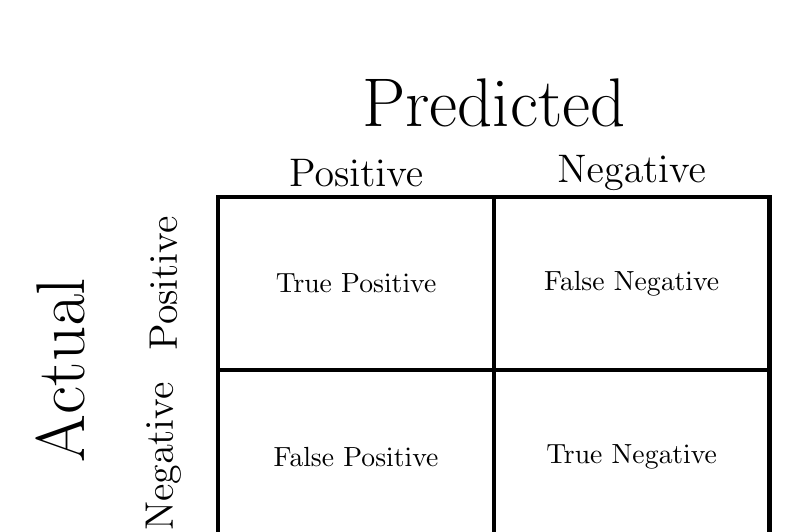
\begin{tikzpicture}[>=stealth]
    \def\w{3.5}
    \def\h{2.2}
    % Column headings
    \node at (3.5, 5.6) {\Huge{Predicted}};
    \node at (1.75, 4.7) {\Large Positive};
    \node at (5.25, 4.7) {\Large Negative};

    % Row headings
    \node[rotate=90] at (-2.0, 2.2) {\Huge{Actual}};
    \node[rotate=90] at (-0.7, 3.3) {\Large Positive};
    \node[rotate=90] at (-0.7, 1.1) {\Large Negative};

    % Matrix
    \draw[line width=1.5pt] (0,0) rectangle (7,4.4);
    \draw[line width=1.5pt] (3.5,0) -- (3.5,4.4);
    \draw[line width=1.5pt] (0,2.2) -- (7,2.2);

    % Entries
    \node at (1.75,3.3) {True Positive};
    \node at (5.25,3.3) {False Negative};
    \node at (1.75,1.1) {False Positive};
    \node at (5.25,1.1) {True Negative};
\end{tikzpicture}
\end{center}
    \caption{Confusion matrix}
\end{figure}
\end{definition}
It shows where the model or test made correct predictions and where it was wrong. This summary helps you understand whether it confuses positive and negatives, helping you improve its accuracy. Also check \url{https://en.wikipedia.org/wiki/Confusion_matrix}. There are few metrics based on confusion matrix.

\begin{definition}
    The \emph{accuracy}\index{accuracy} is defined as 
    \begin{align}
        \text{accuracy} &\defn \frac{\mathrm{TP} + \mathrm{TN}}{\mathrm{TP} + \mathrm{TN} + \mathrm{FP} + \mathrm{FN}}
    \end{align}
\end{definition}
Accuracy shows how many predictions the model got right out of all the predictions. It gives idea of overall performance but it can be misleading when one class is more dominant over the other. For example a model that predicts the majority class correctly most of the time might have high accuracy but still fail to capture important details about other classes. 
\begin{example}[Accuracy of a spam filter]
    A spam filter is evaluated on $1{,}000$ emails and produces
    $\mathrm{TP}=80$, $\mathrm{FP}=15$, $\mathrm{FN}=5$, and $\mathrm{TN}=900$.
    Its accuracy is
    \begin{align}
        \frac{80+900}{80+15+5+900} = \frac{980}{1000} = 0.98.
    \end{align}
    That is, $98\%$ of all predictions are correct.
\end{example}

\begin{example}[Accuracy with imbalanced classes]
    On a fraud dataset with $990$ legitimate transactions and $10$ fraudulent
    ones, the classifier that always predicts ``legitimate'' has
    $\mathrm{TN}=990$, $\mathrm{TP}=0$, and accuracy $990/1000=0.99$. It is
    nevertheless useless for fraud detection because it never identifies a
    fraudulent transaction. This is why accuracy should be reported together
    with precision and recall on imbalanced data.
\end{example}

\begin{definition}
    The \emph{precision}\index{precision} is defined as
    \begin{align}
        \mathrm{precision} &\defn \frac{\mathrm{TP}}{\mathrm{TP}+\mathrm{FP}}
    \end{align}
\end{definition}
Precision focus on the quality of the model’s positive predictions. It tells us how many of the ``positive'' predictions were actually correct. It is important in situations where false positives need to be minimized such as detecting spam emails or fraud.
\begin{example}[Precision of a spam filter]
    Suppose a spam filter has $\mathrm{TP}=90$, $\mathrm{FP}=10$,
    $\mathrm{FN}=30$, and $\mathrm{TN}=870$. Then
    \begin{align}
        \mathrm{precision} = \frac{90}{90+10} = 0.90.
    \end{align}
    Of the $100$ emails that the filter flags as spam, $90$ really are spam.
\end{example}

\begin{example}[Precision and low disease prevalence]
    A screening test is applied to $10{,}000$ people. It gives
    $\mathrm{TP}=18$, $\mathrm{FP}=182$, $\mathrm{FN}=2$, and
    $\mathrm{TN}=9798$, so
    \begin{align}
        \mathrm{precision} = \frac{18}{18+182} = 0.09.
    \end{align}
    Although the test finds $18$ of the $20$ diseased people, only $9\%$ of the
    positive test results are true positives. When the disease is rare, even a
    modest false-positive rate can dominate the positive predictions.
\end{example}

\begin{definition}
    The \emph{recall}\index{recall} is defined as
    \begin{align}
        \mathrm{recall} &\defn \frac{\mathrm{TP}}{\mathrm{TP}+\mathrm{FN}}
    \end{align}
\end{definition}
\begin{example}[Recall of a disease test]
    With $\mathrm{TP}=60$, $\mathrm{FN}=40$, $\mathrm{FP}=20$, and
    $\mathrm{TN}=880$,
    \begin{align}
        \mathrm{recall} = \frac{60}{60+40} = 0.60.
    \end{align}
    The test finds $60\%$ of all people who actually have the disease.
\end{example}

\begin{example}[Recall of a fire alarm]
    A fire-alarm system that misses one fire in five has recall $0.8$. A second
    system that misses one fire in twenty has recall $0.95$. When false negatives
    are dangerous, recall is the key metric even if the more sensitive system
    produces more false alarms.
\end{example}

\begin{definition}
    The \emph{$\mathrm{F1}$-score}\index{F1-score} is defined as
    \begin{align}
        \mathrm{F1} &\defn 2 \cdot \frac{\mathrm{precision} \cdot \mathrm{recall}}{\mathrm{precision} + \mathrm{recall}}
    \end{align}
    It is defined as the harmonic mean of precision and recall.
\end{definition}
F1-score combines precision and recall into a single metric to balance their trade-off. It provides a better sense of a model’s overall performance particularly for imbalanced datasets. It is helpful when both false positives and false negatives are important though it assumes precision and recall are equally important but in some situations one might matter more than the other.
\begin{example}[Computing the F1-score]
    For a classifier with $\mathrm{TP}=40$, $\mathrm{FP}=10$, $\mathrm{FN}=20$,
    and $\mathrm{TN}=930$,
    \begin{align}
        \mathrm{precision} = \frac{40}{50} = 0.80,
        \qquad
        \mathrm{recall} = \frac{40}{60} = 0.667,
    \end{align}
    and therefore
    \begin{align}
        \mathrm{F1}
        = 2\cdot\frac{0.80\cdot0.667}{0.80+0.667}
        \approx 0.727.
    \end{align}
\end{example}

\begin{example}[F1-score versus a single metric]
    Model~A has precision $0.9$ and recall $0.2$, so its F1-score is
    $2(0.9)(0.2)/(0.9+0.2)\approx0.327$. Model~B has precision $0.6$ and recall
    $0.6$, so its F1-score is $0.6$. The F1-score prefers Model~B because it
    rewards balanced performance, whereas Model~A is excellent at avoiding false
    positives but misses most positive cases.
\end{example}

\begin{definition}
    The \emph{specificity}\index{specificity} is defined as
    \begin{align}
        \mathrm{specificity} &\defn \frac{\mathrm{TN}}{\mathrm{TN}+\mathrm{FP}}
    \end{align}
\end{definition}
Specificity is another important metric in the evaluation of classification models particularly in binary classification. It measures the ability of a model to correctly identify negative instances. Specificity is also known as the True Negative Rate Formula.
\begin{example}[Specificity of a screening test]
    A test with $\mathrm{TN}=935$, $\mathrm{FP}=5$, $\mathrm{TP}=50$, and
    $\mathrm{FN}=10$ has
    \begin{align}
        \mathrm{specificity} = \frac{935}{935+5} = 0.9947.
    \end{align}
    It correctly clears $99.47\%$ of the healthy people.
\end{example}

\begin{example}[Specificity and confirmatory tests]
    A confirmatory test that rarely raises false alarms can have very high
    specificity; for example, $\mathrm{TN}=9990$ and $\mathrm{FP}=10$ give
    specificity $0.999$. Specificity is especially important when a false
    positive triggers costly or invasive follow-up tests.
\end{example}

\begin{definition}
    The \emph{Matthews correlation coefficient}\index{Matthews correlation coefficient} is defined as
    \begin{align}
        \mathrm{MCC} &\defn \frac{\mathrm{TP} \cdot \mathrm{TN} - \mathrm{FP} \cdot \mathrm{FN}}{\sqrt{(\mathrm{TP} + \mathrm{FP})(\mathrm{TP} + \mathrm{FN})(\mathrm{TN} + \mathrm{FP})(\mathrm{TN} + \mathrm{FN})}}
    \end{align}
\end{definition}
The Matthews correlation coefficient is a measure of the quality of binary classifications. It takes into account true and false positives and negatives and is generally regarded as a balanced measure which can be used even if the classes are of very different sizes.
\begin{example}[Computing the MCC]
    Using $\mathrm{TP}=40$, $\mathrm{FP}=10$, $\mathrm{FN}=20$, and
    $\mathrm{TN}=930$,
    \begin{align}
        \mathrm{MCC}
        &= \frac{40\cdot930 - 10\cdot20}
                {\sqrt{(50)(60)(940)(980)}} \\
        &= \frac{37000}{52570} \approx 0.704.
    \end{align}
    The value is well above zero, indicating a genuine association between the
    predictions and the labels.
\end{example}

\begin{example}[MCC for random guessing]
    On a balanced test set with $\mathrm{TP}=25$, $\mathrm{FP}=25$,
    $\mathrm{FN}=25$, and $\mathrm{TN}=25$,
    \begin{align}
        \mathrm{MCC}
        = \frac{25\cdot25 - 25\cdot25}
               {\sqrt{(50)(50)(50)(50)}} = 0.
    \end{align}
    Random guessing therefore receives an MCC of zero, while a lopsided
    classifier can still appear to have high accuracy.
\end{example}

\begin{definition}
    The \emph{Type-1 error probability} $\epsilon_1$ is defined as
    \begin{align}
        \epsilon_1 &\defn \frac{\mathrm{FP}}{\mathrm{FP} + \mathrm{TN}}
    \end{align}
    and the \emph{Type-2 error probability} $\epsilon_2$ is defined as
    \begin{align}
        \epsilon_2 &\defn \frac{\mathrm{FN}}{\mathrm{FN} + \mathrm{TP}}
    \end{align}
\end{definition}
Type 1 error occurs when the model incorrectly predicts a positive instance but the actual instance is negative. This is also known as a false positive. Type 1 Errors affect the precision of a model which measures the accuracy of positive predictions. Type 2 error occurs when the model fails to predict a positive instance even though it is actually positive. This is also known as a false negative. Type 2 Errors impact the recall of a model which measures how well the model identifies all actual positive cases.
\begin{example}[Type-1 and Type-2 error probabilities]
    With $\mathrm{TP}=45$, $\mathrm{FP}=5$, $\mathrm{FN}=15$, and
    $\mathrm{TN}=935$,
    \begin{align}
        \epsilon_1 &= \frac{5}{5+935} = \frac{5}{940} \approx 0.0053, \\
        \epsilon_2 &= \frac{15}{15+45} = \frac{15}{60} = 0.25.
    \end{align}
    The test has a low false-positive rate but misses $25\%$ of the true
    positive cases.
\end{example}

\begin{example}[Errors in a criminal trial]
    In a criminal trial, a Type-1 error is convicting an innocent defendant and
    a Type-2 error is acquitting a guilty one. Lowering the standard of evidence
    reduces Type-2 errors but increases Type-1 errors, and raising it has the
    opposite effect. This is the same trade-off as moving a classifier's decision
    threshold.
\end{example}

\section{Bias--variance decomposition}

Bias is the error caused by simplifying assumptions built into the model. Variance is
how much the learned function changes if it is trained on a different training set.
For squared loss, with $y = f(\mathbf{x}) + \varepsilon$,
$\E[\varepsilon]=0$, $\Var(\varepsilon)=\sigma^2$, the expected test error at a point
$\mathbf{x}$ decomposes as
\begin{align}
    \E\big[(y - \hat{f}(\mathbf{x}))^2\big]
    = \underbrace{\big(\E[\hat{f}(\mathbf{x})] - f(\mathbf{x})\big)^2}_{\text{bias}^2}
    + \underbrace{\Var\big(\hat{f}(\mathbf{x})\big)}_{\text{variance}}
    + \underbrace{\sigma^2}_{\text{irreducible noise}}.
\end{align}
The expectation is over the randomness of the training set and the noise.

\begin{figure}[htbp]
\centering
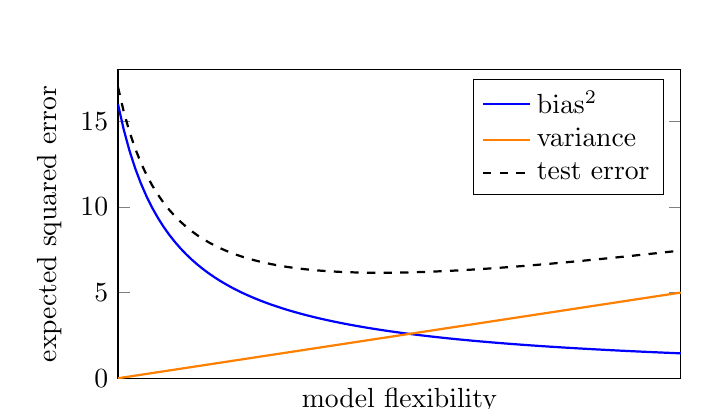
\begin{tikzpicture}
\begin{axis}[
    width=0.72\textwidth, height=5.5cm,
    xlabel={model flexibility}, ylabel={expected squared error},
    domain=0:10, samples=100,
    xmin=0, xmax=10, ymin=0, ymax=18,
    xtick=\empty, ytick={0,5,10,15},
    legend pos=north east, legend cell align=left
]
\addplot[thick, blue] {16/(x+1)};
\addlegendentry{bias$^2$}
\addplot[thick, orange] {0.5*x};
\addlegendentry{variance}
\addplot[thick, black, dashed] {16/(x+1)+0.5*x+1};
\addlegendentry{test error}
\end{axis}
\end{tikzpicture}
\caption{As model flexibility grows, squared bias falls and variance rises; their sum plus irreducible noise is minimised at an intermediate complexity.}
\label{fig:bias-variance}
\end{figure}

Generally, more flexible methods have more variance and less bias; less flexible
methods have more bias and less variance. The best method for a task balances the two
to achieve the lowest test error (Figure~\ref{fig:bias-variance}). This is why
regularisation (Chapter~\ref{ch:reg}) and cross-validation
(Chapter~\ref{ch:cv}) are central tools.

\section{The curse of dimensionality}

As dimensionality increases, data become sparse: to maintain a given density of
samples, the number of observations must grow exponentially with the number of
dimensions. Distance-based methods such as k-NN deteriorate because nearest
neighbours are no longer meaningfully ``near''. The curse of dimensionality motivates
dimensionality reduction, feature selection, strong inductive biases, and models that
share parameters across dimensions.

\section{Common trade-offs}

\begin{enumerate}
    \item Bias versus variance.
    \item Accuracy versus interpretability.
    \item Accuracy versus scalability.
    \item Domain knowledge versus data-driven learning.
    \item More data versus a better algorithm.
    \item Accuracy versus fairness, privacy, and robustness.
\end{enumerate}
There is no universally best point on these axes. The right choice depends on the
deployment context, the cost of different errors, and the available data.

\chapter{Linear Regression}
\label{ch:linear}

Linear regression is a simple supervised-learning method for predicting quantitative
outputs. Many machine-learning methods are generalisations of it, and it illustrates
key concepts---least squares, overfitting, regularisation, and inference---while
remaining interpretable.

\section{Simple linear regression}

Simple linear regression predicts a quantitative response $Y$ from a single predictor
$X$, assuming an approximately linear relationship:
\begin{align}
    Y = \beta_0 + \beta_1 X + \epsilon.
\end{align}
Here $\beta_0$ is the intercept and $\beta_1$ the slope; together they are the
\emph{coefficients} or \emph{parameters} of the model. We estimate them from training
data
\begin{align}
    (x^{(1)}, y^{(1)}), \ldots, (x^{(n)}, y^{(n)}).
\end{align}
Estimated parameters are denoted $\hat{\beta}_0, \hat{\beta}_1$. For a realisation
$X=x$, the prediction is
\begin{align}
    \hat{y} = \hat{\beta}_0 + \hat{\beta}_1 x.
\end{align}
The goal is to choose the coefficients so that
$y^{(i)} \approx \hat{\beta}_0 + \hat{\beta}_1 x^{(i)}$ for all $i$. Two questions
remain: how do we estimate the coefficients (\emph{fit} the model), and what counts
as a \emph{good fit}?

The usual assumptions are: linearity in the parameters, independent errors,
constant error variance (homoscedasticity), and---for exact inference---normally
distributed errors. The predictor may be transformed (logs, polynomials) while the
model remains linear in $\beta$.

\section{Least squares}

\begin{definition}[Residuals and RSS]
The \emph{residual} for the $i$-th observation is
\begin{align}
    e^{(i)} = y^{(i)} - \hat{y}^{(i)}.
\end{align}
The \emph{residual sum of squares} (RSS) is
\begin{align}
    \mathrm{RSS}
    = \sum_{i=1}^n (e^{(i)})^2
    = \sum_{i=1}^n \big(y^{(i)} - \hat{y}^{(i)}\big)^2.
\end{align}
\end{definition}

\begin{definition}[Least-squares estimator]
The least-squares estimates jointly minimise the RSS:
\begin{align}
    (\hat{\beta}_0, \hat{\beta}_1)
    = \arg\min_{\beta_0,\beta_1}
    \sum_{i=1}^n \big(y^{(i)} - \beta_0 - \beta_1 x^{(i)}\big)^2.
\end{align}
\end{definition}

Setting the partial derivatives to zero gives the normal equations. For simple
linear regression their solution is
\begin{align}
    \hat{\beta}_1
    &= \frac{\sum_{i=1}^n (x^{(i)} - \bar{x})(y^{(i)} - \bar{y})}
              {\sum_{i=1}^n (x^{(i)} - \bar{x})^2}
    = \frac{\Cov(x,y)}{\Var(x)},\\
    \hat{\beta}_0 &= \bar{y} - \hat{\beta}_1 \bar{x}.
\end{align}
The fitted line always passes through $(\bar{x},\bar{y})$. The second derivative of
the RSS with respect to $\beta_1$ is $2\sum_i (x^{(i)}-\bar{x})^2 > 0$, so the
stationary point is a minimum.

\section{Multiple linear regression}

With $p$ predictors, write each observation as a row of a design matrix
$\mathbf{X} \in \R^{n \times (p+1)}$ (the leading column of ones absorbs the
intercept) and the targets as $\mathbf{y} \in \R^n$. Then
\begin{align}
    \mathbf{y} = \mathbf{X}\boldsymbol{\beta} + \boldsymbol{\epsilon},
    \qquad
    \mathrm{RSS}(\boldsymbol{\beta})
    = (\mathbf{y} - \mathbf{X}\boldsymbol{\beta})^\top
      (\mathbf{y} - \mathbf{X}\boldsymbol{\beta}).
\end{align}
Differentiating with respect to $\boldsymbol{\beta}$ and setting the result to zero
gives the \emph{normal equations}
\begin{align}
    \mathbf{X}^\top\mathbf{X}\boldsymbol{\beta}
    = \mathbf{X}^\top\mathbf{y},
\end{align}
so, when $\mathbf{X}^\top\mathbf{X}$ is invertible,
\begin{align}
    \hat{\boldsymbol{\beta}}
    = (\mathbf{X}^\top\mathbf{X})^{-1}\mathbf{X}^\top\mathbf{y}.
\end{align}
The fitted values are $\hat{\mathbf{y}} = \mathbf{H}\mathbf{y}$ with the \emph{hat
matrix} $\mathbf{H} = \mathbf{X}(\mathbf{X}^\top\mathbf{X})^{-1}\mathbf{X}^\top$.
The hat matrix is symmetric and idempotent, $\mathbf{H}^2=\mathbf{H}$, and projects
$\mathbf{y}$ onto the column space of $\mathbf{X}$.

If $\mathbf{X}^\top\mathbf{X}$ is singular or nearly singular (collinearity, more
features than observations), the inverse is unstable or does not exist. Ridge
regression (Chapter~\ref{ch:reg}) fixes this by adding $\lambda\mathbf{I}$.

\section{Coefficient interpretation and inference}

In multiple regression, $\beta_j$ is the expected change in $Y$ associated with a
one-unit increase in $X_j$, \emph{holding all other predictors fixed}. This
``holding fixed'' clause is essential; with correlated predictors the coefficients can
change substantially when predictors are added or removed.

Under the classical assumptions, the least-squares estimator is unbiased,
$\E[\hat{\boldsymbol{\beta}}]=\boldsymbol{\beta}$, with covariance
\begin{align}
    \Var(\hat{\boldsymbol{\beta}})
    = \sigma^2(\mathbf{X}^\top\mathbf{X})^{-1}.
\end{align}
Replacing $\sigma^2$ by its estimate
$\hat{\sigma}^2 = \mathrm{RSS}/(n-p-1)$ gives standard errors. A $t$-statistic
$\hat{\beta}_j/\mathrm{SE}(\hat{\beta}_j)$ tests whether a single coefficient is
zero; an $F$-test compares a full model with a nested model. These tests are valid
only if the model assumptions are reasonable.

Two summary measures are common:
\begin{enumerate}
    \item \emph{Residual standard error} (RSE):
    \begin{align}
        \mathrm{RSE}
        = \sqrt{\frac{\mathrm{RSS}}{n-p-1}}
        = \sqrt{\frac{1}{n-p-1}\sum_{i=1}^n (y^{(i)} - \hat{y}^{(i)})^2}.
    \end{align}
    A higher RSE means a worse fit on the scale of $Y$.
    \item \emph{Coefficient of determination} $R^2$:
    \begin{align}
        R^2 = \frac{\mathrm{TSS} - \mathrm{RSS}}{\mathrm{TSS}}
        = 1 - \frac{\mathrm{RSS}}{\mathrm{TSS}},
        \qquad
        \mathrm{TSS} = \sum_{i=1}^n (y^{(i)} - \bar{y})^2.
    \end{align}
    $R^2$ is the proportion of variability in $Y$ explained by the model. It always
    increases when predictors are added, so the \emph{adjusted} $R^2$ penalises model
    size:
    \begin{align}
        R^2_{\mathrm{adj}}
        = 1 - (1-R^2)\frac{n-1}{n-p-1}.
    \end{align}
\end{enumerate}

\section{Diagnostics and extensions}

Residual plots reveal violations of the assumptions. A funnel shape suggests
heteroscedasticity; curvature suggests a missing nonlinear term; a few large residuals
suggest outliers or high-leverage points. Diagnostic plots are more informative than
$R^2$ alone.

Linear regression can be extended without leaving the linear-in-parameters
framework:
\begin{itemize}
    \item \textbf{Polynomial and spline terms}: add $x^2, x^3, \ldots$ or spline basis
    functions.
    \item \textbf{Interactions}: add products $x_j x_k$ to model non-additive effects.
    \item \textbf{Qualitative predictors}: encode categories with dummy variables
    (one-hot encoding), dropping one level to avoid collinearity.
    \item \textbf{Generalised linear models}: replace the Gaussian likelihood and
    identity link; logistic regression is the Bernoulli case
    (Chapter~\ref{ch:logistic}).
\end{itemize}

\section{Strengths and limitations}

Linear regression is fast, interpretable, and a strong baseline. It is easy to
regularise and has well-understood statistical theory. Its main limitation is the
linearity assumption: it cannot capture complex interactions unless they are
engineered explicitly. It is also sensitive to outliers and to collinearity, and it
can overfit when $p$ is large relative to $n$.

\coderef{Code/linear_regression.py}
\coderef{Code/linear_regression.ipynb}

\chapter{Logistic Regression and Classification}
\label{ch:logistic}

\section{Classification setup}

In binary classification the target is $y \in \{0,1\}$. A linear model
\begin{align}
    \hat{y} = \mathbf{w}^\top\mathbf{x} + b
\end{align}
can take any real value, so it is not a
probability. Applying a threshold gives a classifier, but the resulting decision
boundary is still linear and the model is sensitive to the scale of the scores. We
want a model that outputs a probability in $(0,1)$ and a loss that is appropriate for
labels.

\section{The logistic model}

The \emph{logistic (sigmoid) function} is
\begin{align}
    \sigma(z) \defn \frac{1}{1+e^{-z}}.
\end{align}
It is increasing, maps $\R$ to $(0,1)$, and satisfies
\begin{align}
    \sigma'(z)=\sigma(z)(1-\sigma(z)).
\end{align}
Logistic regression models
\begin{align}
    \Pr(Y=1\mid\mathbf{x}) = \sigma(\mathbf{w}^\top\mathbf{x} + b)
    = \frac{1}{1+e^{-(\mathbf{w}^\top\mathbf{x}+b)}}.
\end{align}
The \emph{log-odds} (logit) are linear:
\begin{align}
    \log\frac{\Pr(Y=1\mid\mathbf{x})}{\Pr(Y=0\mid\mathbf{x})}
    = \mathbf{w}^\top\mathbf{x} + b.
\end{align}
A one-unit increase in $x_j$ multiplies the odds by $e^{w_j}$, holding the other
features fixed. This is a useful interpretation that linear regression does not
provide for probabilities.

The decision boundary is the set where $\Pr(Y=1\mid\mathbf{x})=1/2$, i.e.
$\mathbf{w}^\top\mathbf{x}+b=0$, which is a hyperplane. Logistic regression is
therefore a \emph{linear classifier}, but a probabilistic one.

\begin{figure}[htbp]
\centering
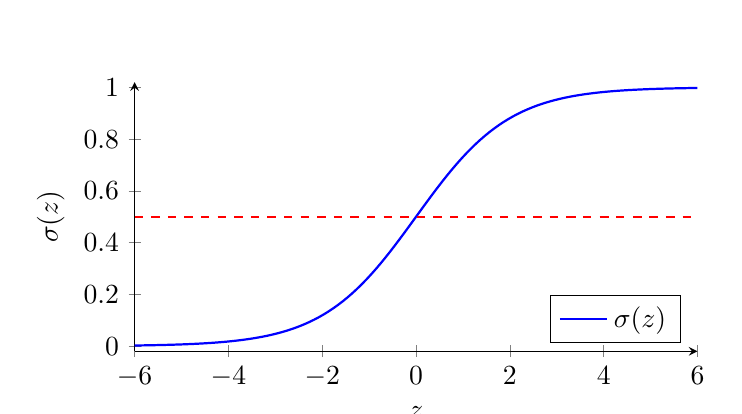
\begin{tikzpicture}
\begin{axis}[
    width=0.72\textwidth, height=5cm,
    xlabel={$z$}, ylabel={$\sigma(z)$},
    domain=-6:6, samples=120, ymin=-0.02, ymax=1.02,
    axis lines=left, legend pos=south east
]
\addplot[thick, blue] {1/(1+exp(-x))};
\addlegendentry{$\sigma(z)$}
\addplot[thick, red, dashed] {0.5};
\end{axis}
\end{tikzpicture}
\caption{The logistic sigmoid. The decision threshold $0.5$ corresponds to $z=0$.}
\label{fig:sigmoid}
\end{figure}

\section{Maximum likelihood and cross-entropy}

\begin{definition}
    For a dataset $D = \{(\mathbf{x}^{(i)},y_i)\}_{i=1}^n$, the likelihood is
    \begin{align}
        L(\mathbf{w},b) \defn \prod_{i=1}^n p_i^{y_i}(1-p_i)^{1-y_i},
    \end{align}
    where $p_i = \sigma(\mathbf{w}^\top\mathbf{x}^{(i)}+b)$.
\end{definition}

\begin{example}[Likelihood for two observations]
    Suppose $n=2$, with labels $y_1=1$ and $y_2=0$, and predicted probabilities
    $p_1=0.9$ and $p_2=0.2$. Then
    \begin{align}
        L(\mathbf{w},b)
        = p_1^{1}(1-p_1)^{0}\,p_2^{0}(1-p_2)^{1}
        = 0.9 \cdot 0.8 = 0.72.
    \end{align}
    The log-likelihood is $\log 0.72 \approx -0.329$.
\end{example}

\begin{example}[Likelihood rewards confident correct predictions]
    For a single example with label $y=1$, a predicted probability $p=0.99$
    gives likelihood $0.99$, while $p=0.51$ gives likelihood $0.51$. Maximising
    the likelihood therefore rewards assigning high probability to the observed
    label. Note that the likelihood is a function of the parameters, not a
    probability distribution over them.
\end{example}

\begin{definition}
    Given a dataset $D = \{(\mathbf{x}^{(i)},y_i)\}_{i=1}^n$, the \emph{binary cross-entropy}\index{binary cross-entropy} is
    \begin{align}
        \ell(\mathbf{w},b) \defn -\sum_{i=1}^n \left[ y_i \log p_i + (1-y_i)\log(1-p_i) \right],
    \end{align}
    where $p_i = \sigma(\mathbf{w}^\top\mathbf{x}^{(i)}+b)$.
\end{definition}

\begin{example}[Binary cross-entropy for two observations]
    Using the same two observations as above, with $(y_1,p_1)=(1,0.9)$ and
    $(y_2,p_2)=(0,0.2)$,
    \begin{align}
        \ell(\mathbf{w},b)
        &= -\big[\log 0.9 + \log(1-0.2)\big] \\
        &= -\big[-0.1054 - 0.2231\big]
        = 0.3285.
    \end{align}
    This is exactly the negative log-likelihood, so minimising the cross-entropy
    is the same as maximising the likelihood.
\end{example}

\begin{example}[Confident mistakes are penalised heavily]
    For a correctly classified example with $y=1$ and $p=0.99$, the loss is
    $-\log 0.99 \approx 0.010$. For a confidently wrong prediction with $y=1$
    and $p=0.01$, the loss is $-\log 0.01 \approx 4.605$. The loss grows without
    bound as the predicted probability of the correct class approaches zero,
    which is why cross-entropy strongly discourages confident mistakes.
\end{example}

Maximising the log-likelihood is equivalent to minimising the \emph{binary cross-entropy}.

The gradient\index{gradient} of the binary cross-entropy has the clean form
\begin{align}
    \nabla_{\mathbf{w}} \ell
    = \sum_{i=1}^n (p_i - y_i)\,\mathbf{x}^{(i)},
    \qquad
    \frac{\partial \ell}{\partial b}
    = \sum_{i=1}^n (p_i - y_i).
\end{align}
Unlike linear regression, there is no closed-form solution; we use gradient descent,
Newton's method, or a specialised solver such as L-BFGS. The negative log-likelihood
is convex in $(\mathbf{w},b)$, so a local minimum is global.

Regularised logistic regression adds $\lambda\norm{\mathbf{w}}_2^2$ or
$\lambda\norm{\mathbf{w}}_1$ to the objective. The intercept is normally not
penalised. Regularisation is important when the classes are separable, because the
unregularised maximum-likelihood solution can have infinite weights.

\section{Multiclass logistic regression}

For $m$ classes, use the \emph{softmax} function:
\begin{align}
    \Pr(Y=k\mid\mathbf{x})
    = \frac{e^{\mathbf{w}_k^\top\mathbf{x}+b_k}}
           {\sum_{j=1}^m e^{\mathbf{w}_j^\top\mathbf{x}+b_j}}.
\end{align}
The loss is the categorical cross-entropy
\begin{align}
    \ell = -\sum_{i=1}^n \log \Pr(Y=y_i\mid\mathbf{x}^{(i)}).
\end{align}
Softmax regression has one parameter vector per class; the parameters are
identifiable only up to a common additive constant unless a reference class or a
regulariser is used.

\section{Evaluating classifiers}

Accuracy is the fraction of correct predictions, but it can be misleading when classes
are imbalanced. For binary classification, define
\begin{align}
    \mathrm{precision} &= \frac{\mathrm{TP}}{\mathrm{TP}+\mathrm{FP}}, &
    \mathrm{recall} &= \frac{\mathrm{TP}}{\mathrm{TP}+\mathrm{FN}},\\
    F_1 &= \frac{2\,\mathrm{precision}\cdot\mathrm{recall}}
                {\mathrm{precision}+\mathrm{recall}}, &
    \mathrm{specificity} &= \frac{\mathrm{TN}}{\mathrm{TN}+\mathrm{FP}}.
\end{align}
The \emph{confusion matrix} tabulates true and predicted labels and is often more
informative than a single number.

A probabilistic classifier outputs scores; varying the threshold traces a
\emph{receiver operating characteristic} (ROC) curve of true-positive rate against
false-positive rate. The area under this curve (AUC) is a threshold-independent
summary. For heavily imbalanced data, the precision--recall curve is often more
informative than ROC. \emph{Calibration} asks whether predicted probabilities match
observed frequencies; a model can rank well yet be badly calibrated.

\section{Class imbalance and practical issues}

When one class is rare, a classifier that always predicts the majority class can have
high accuracy but be useless. Remedies include resampling, class weights, threshold
tuning, and choosing a loss that reflects the relative cost of errors. Always report
metrics beyond accuracy, and always evaluate on a held-out set with the same class
distribution as deployment.

\coderef{Code/logistic_regression.py}
\coderef{Code/mnist_supervised.py}

\chapter{Regularization and Sparsity}
\label{ch:reg}

Regularisation penalises model complexity to reduce variance and combat overfitting.
We add a penalty $P(\boldsymbol{\beta})$ to the training objective:
\begin{align}
    \hat{\boldsymbol{\beta}}
    = \arg\min_{\boldsymbol{\beta}}
      \left\{ \mathrm{RSS}(\boldsymbol{\beta})
      + \lambda\,P(\boldsymbol{\beta}) \right\},
\end{align}
where $\lambda \geq 0$ controls the strength of regularisation. Equivalently, for a
given budget $t$,
\begin{align}
    \min_{\boldsymbol{\beta}} \mathrm{RSS}(\boldsymbol{\beta})
    \quad \text{subject to} \quad P(\boldsymbol{\beta}) \leq t.
\end{align}
This is the Lagrangian form of a constrained optimisation problem. Larger $\lambda$
means a smaller feasible region and stronger shrinkage.

\section{Ridge regression ($\ell_2$)}

Ridge regression uses
\begin{align}
    P(\boldsymbol{\beta}) = \sum_{j=1}^p \beta_j^2 = \norm{\boldsymbol{\beta}}_2^2.
\end{align}
The objective is
\begin{align}
    \mathrm{RSS}(\boldsymbol{\beta}) + \lambda\norm{\boldsymbol{\beta}}_2^2,
\end{align}
with closed-form solution
\begin{align}
    \hat{\boldsymbol{\beta}}_{\mathrm{ridge}}
    = (\mathbf{X}^\top\mathbf{X} + \lambda\mathbf{I})^{-1}\mathbf{X}^\top\mathbf{y}
\end{align}
when the intercept is handled separately. The added $\lambda\mathbf{I}$ makes the
matrix invertible even when $\mathbf{X}^\top\mathbf{X}$ is singular. Ridge shrinks
coefficients toward zero but rarely sets them exactly to zero. It is effective when
many predictors have small, non-zero effects, and it handles correlated predictors
gracefully by distributing weight among them.

Ridge has a Bayesian interpretation: it is the MAP estimate under a Gaussian prior
$\beta_j \sim \mathscr{N}(0,\tau^2)$ with $\lambda = \sigma^2/\tau^2$.

\section{LASSO ($\ell_1$)}

The LASSO (least absolute shrinkage and selection operator) uses
\begin{align}
    P(\boldsymbol{\beta}) = \sum_{j=1}^p |\beta_j| = \norm{\boldsymbol{\beta}}_1.
\end{align}
Unlike ridge, LASSO can set coefficients exactly to zero, performing automatic
\emph{feature selection}. The solution is \emph{sparse}: only a subset of predictors
retain non-zero coefficients. This is valuable for interpretation and for
high-dimensional problems, but LASSO can behave erratically when predictors are
highly correlated: it tends to select one and ignore the others.

LASSO is the MAP estimate under a Laplace prior,
$p(\beta_j) \propto e^{-|\beta_j|/b}$. The Laplace density has a sharp peak at zero,
which is the probabilistic counterpart of the geometric corner argument below.

\section{Elastic net}

Elastic net combines both penalties:
\begin{align}
    P(\boldsymbol{\beta})
    = \alpha\norm{\boldsymbol{\beta}}_1 + (1-\alpha)\norm{\boldsymbol{\beta}}_2^2,
\end{align}
interpolating between LASSO ($\alpha=1$) and ridge ($\alpha=0$). It handles
correlated predictors better than LASSO alone, because the $\ell_2$ term encourages
groups of correlated variables to enter or leave together, while the $\ell_1$ term
still produces sparsity.

\section{Why the $\ell_1$ penalty yields sparsity}

The $\ell_1$ ball $\{\boldsymbol{\beta}: \norm{\boldsymbol{\beta}}_1 \leq t\}$ has
corners on the coordinate axes; the contours of the unpenalised loss tend to touch
these corners, forcing some coefficients to zero. The $\ell_2$ ball is round, so
contact typically occurs with all coefficients non-zero. In two dimensions, the
picture is:

\begin{figure}[htbp]
\centering
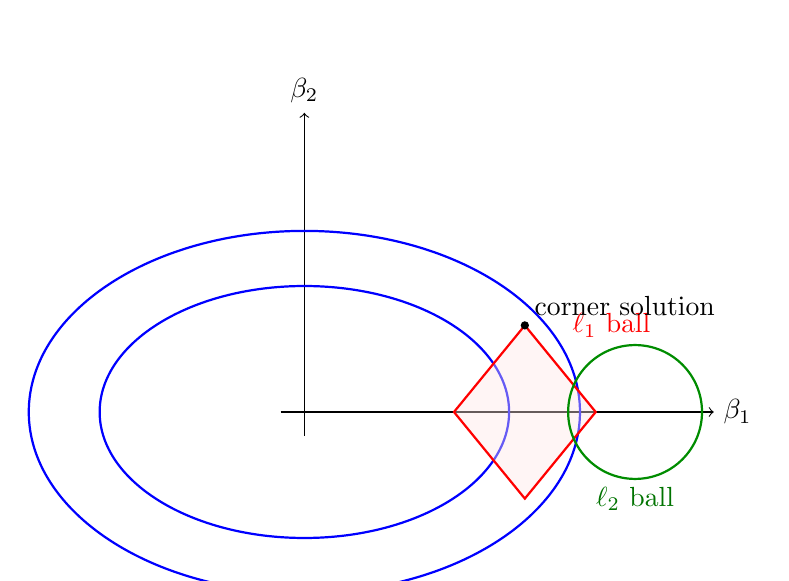
\begin{tikzpicture}[scale=1.0]
\draw[->] (-0.3,0) -- (5.2,0) node[right] {$\beta_1$};
\draw[->] (0,-0.3) -- (0,3.8) node[above] {$\beta_2$};
\draw[thick, blue] (0,0) ellipse (2.6 and 1.6);
\draw[thick, blue] (0,0) ellipse (3.5 and 2.3);
\draw[thick, red, fill=red!10, fill opacity=0.4]
  (1.9,0) -- (2.8,1.1) -- (3.7,0) -- (2.8,-1.1) -- cycle;
\node[red] at (3.9,1.1) {$\ell_1$ ball};
\draw[thick, green!55!black] (4.2,0) circle (0.85);
\node[green!45!black] at (4.2,-1.1) {$\ell_2$ ball};
\fill (2.8,1.1) circle (1.5pt);
\node[above right] at (2.8,1.1) {corner solution};
\end{tikzpicture}
\caption{Schematic of the constrained view of regularisation. The elliptical
contours are level sets of the loss; the feasible region is the penalty ball. The
$\ell_1$ ball has corners, making sparse solutions likely.}
\label{fig:l1-l2}
\end{figure}

\section{Practical considerations}

\begin{itemize}
    \item \textbf{Standardise features.} Penalties are not scale-invariant. A feature
    measured in thousands will be penalised differently from one measured in
    fractions. Centre and scale before regularising (but do not penalise the
    intercept).
    \item \textbf{Choose $\lambda$ by cross-validation.} The regularisation path is
    usually computed over a grid of $\lambda$ values, and the value with the best
    validation error is selected (Chapter~\ref{ch:cv}).
    \item \textbf{Use the right solver.} Coordinate descent is standard for LASSO;
    `saga` handles elastic net and large sparse problems.
    \item \textbf{Do not interpret selected features as causal.} Selection is
    sensitive to the data and to correlated predictors.
\end{itemize}

\coderef{Code/regularization.py}
\coderef{Code/linear_regression.py}

\chapter{Model Assessment: Cross-Validation and Imputation}
\label{ch:cv}

\section{Why validate?}

Training error optimistically estimates generalisation error, especially for flexible
models. We need held-out data to estimate how well a model performs on unseen
observations. A \emph{validation} set is used for model selection and hyperparameter
tuning; a \emph{test} set is used once, at the end, to report final performance.

\section{Train / validation / test split}

\begin{itemize}
    \item \textbf{Training data}: used to fit model parameters.
    \item \textbf{Validation data}: used to tune hyperparameters and select models.
    \item \textbf{Test data}: used once, at the end, to report final generalisation
    error.
\end{itemize}
The test set must never influence training or hyperparameter choices; otherwise the
reported error is biased downward. When data are scarce, a single validation split is
wasteful, which motivates cross-validation.

\section{k-fold cross-validation}

Partition the data into $k$ roughly equal folds. For each fold $i$:
\begin{enumerate}
    \item Train on the other $k-1$ folds.
    \item Evaluate on fold $i$.
\end{enumerate}
Average the $k$ validation errors to obtain the cross-validation estimate:
\begin{align}
    \mathrm{CV}_{(k)}
    = \frac{1}{k}\sum_{i=1}^k \hat{\risk}_i.
\end{align}
Common choices are $k=5$ or $k=10$; $k=5$ is cheaper, $k=10$ has slightly lower bias.
The folds should be stratified for classification so that each fold preserves the
class proportions, grouped when observations are not independent (for example,
multiple images of the same patient), and ordered when the data are a time series.

\begin{figure}[htbp]
\centering
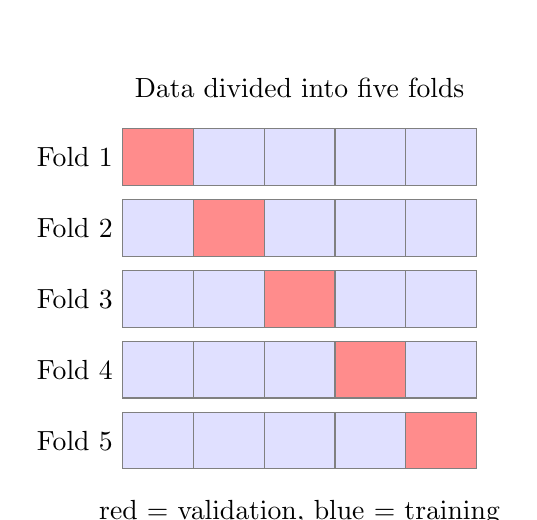
\begin{tikzpicture}[scale=0.9]
\foreach \i in {1,...,5} {
  \foreach \j in {1,...,5} {
    \pgfmathsetmacro{\shade}{(\i==\j) ? 1 : 0}
    \ifnum\shade=1
      \fill[red!45] (\j-1,-\i) rectangle ++(1,0.8);
    \else
      \fill[blue!12] (\j-1,-\i) rectangle ++(1,0.8);
    \fi
    \draw[gray] (\j-1,-\i) rectangle ++(1,0.8);
  }
  \node[left] at (0,-\i+0.4) {Fold \i};
}
\node[above] at (2.5,0.1) {Data divided into five folds};
\node[below] at (2.5,-5.3) {red = validation, blue = training};
\end{tikzpicture}
\caption{Five-fold cross-validation. Each fold serves once as the validation set.}
\label{fig:kfold}
\end{figure}

\section{Leave-one-out cross-validation}

With $k=n$, each observation serves once as the validation set:
\begin{align}
    \mathrm{LOOCV} = \frac{1}{n}\sum_{i=1}^n \ell\big(y_i, \hat{f}^{(-i)}(\mathbf{x}^{(i)})\big).
\end{align}
LOOCV is approximately unbiased but can have high variance because the $n$ training
sets are almost identical. It is computationally expensive ($n$ model fits), although
for ordinary least squares there is a closed-form shortcut using the hat matrix:
\begin{align}
    \mathrm{LOOCV} = \frac{1}{n}\sum_{i=1}^n
    \left(\frac{y_i-\hat{y}_i}{1-h_{ii}}\right)^2,
\end{align}
where $h_{ii}$ is the $i$-th diagonal entry of the hat matrix.

\section{Nested cross-validation}

When both model selection and hyperparameter tuning are needed, use two loops. An
outer loop estimates generalisation error; an inner loop performs cross-validation
for tuning. For each outer fold, the inner loop selects hyperparameters using only
the outer training data. Nested CV prevents information leakage from the tuning step
into the error estimate. It is more expensive but often necessary when comparing many
models.

\section{Data leakage}

Leakage occurs when information from outside the training data influences the model.
Common sources are:
\begin{itemize}
    \item Scaling, imputing, or selecting features before splitting the data.
    \item Using the test set to choose hyperparameters.
    \item Duplicated or near-duplicated observations split across train and test.
    \item Target leakage: a feature that is a proxy for the label or is measured after
    the outcome.
\end{itemize}
The cure is to put every preprocessing step inside a pipeline and fit the pipeline
only on training folds.

\section{Imputation}

Missing data are common. Strategies include:
\begin{itemize}
    \item \textbf{Mean/median imputation}: replace missing values with the feature mean
    or median. Simple but distorts variance and correlations.
    \item \textbf{Mode imputation}: for categorical features, use the most frequent
    category.
    \item \textbf{KNN imputation}: impute from the values of the $k$ nearest complete
    observations.
    \item \textbf{MICE} (multiple imputation by chained equations): model each feature
    with missingness as a function of the others, iterating through features multiple
    times to generate several imputed datasets.
\end{itemize}
Always fit the imputer on training data only, then apply the same transformation to
validation and test data. If the missingness itself is informative, add a
\emph{missing-indicator} feature.

\coderef{Code/cross_validation.py}

\chapter{Support Vector Machines}
\label{ch:svm}

\section{Maximum-margin classification}

For linearly separable binary data with labels $y_i \in \{-1,+1\}$, a hyperplane
\begin{align}
    \mathbf{w}^\top\mathbf{x}+b=0
\end{align}
classifies correctly if
\begin{align}
    y_i(\mathbf{w}^\top\mathbf{x}^{(i)}+b) > 0
\end{align}
for all $i$. Among all separating hyperplanes, the support vector machine chooses the one with the largest \emph{margin}: the distance from the hyperplane to the closest training points. The geometric margin
is $\dfrac{2}{\norm{\mathbf{w}}}$, so maximising the margin is equivalent to minimising $\norm{\mathbf{w}}$.

\begin{figure}[htbp]
\centering
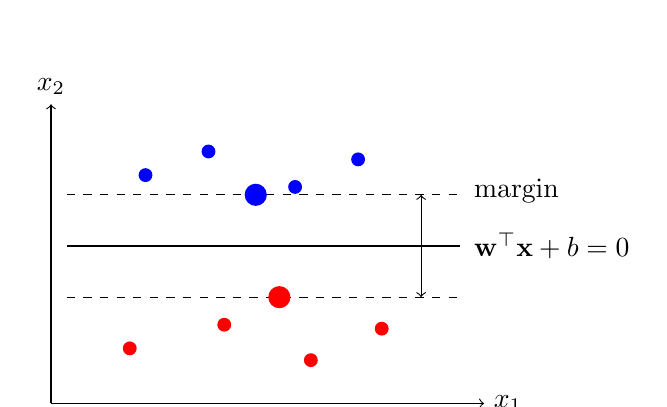
\begin{tikzpicture}[scale=1.0]
\draw[->] (0,0) -- (5.5,0) node[right] {$x_1$};
\draw[->] (0,0) -- (0,3.8) node[above] {$x_2$};
\draw[thick] (0.2,2.0) -- (5.2,2.0);
\draw[dashed] (0.2,1.35) -- (5.2,1.35);
\draw[dashed] (0.2,2.65) -- (5.2,2.65);
\foreach \p in {(1.2,2.9),(2.0,3.2),(3.1,2.75),(3.9,3.1)}
  \fill[blue] \p circle (2.5pt);
\foreach \p in {(1.0,0.7),(2.2,1.0),(3.3,0.55),(4.2,0.95)}
  \fill[red] \p circle (2.5pt);
\fill[blue] (2.6,2.65) circle (4pt);
\fill[red] (2.9,1.35) circle (4pt);
\node[right] at (5.25,2.0) {$\mathbf{w}^\top\mathbf{x}+b=0$};
\node[right] at (5.25,2.7) {margin};
\draw[<->] (4.7,1.35) -- (4.7,2.65);
\end{tikzpicture}
\caption{Schematic of a maximum-margin classifier.}
\label{fig:svm}
\end{figure}


\begin{example}
    \todo{insert a concrete example with small table of data points and graphs.}
\end{example}


\begin{example}
    \todo{insert another concrete example with small table of data points and graphs.}
\end{example}


\section{Hard-margin primal problem}

The hard-margin SVM solves
\begin{align}
    \min_{\mathbf{w},b}\ \frac{1}{2}\norm{\mathbf{w}}^2
    \quad \text{subject to} \quad
    y_i(\mathbf{w}^\top\mathbf{x}^{(i)}+b) \geq 1, \quad i=1,\ldots,n.
\end{align}
The constraints say that every point is on the correct side and at least at unit
distance from the boundary in the scaled coordinates. The objective is strictly convex
and the constraints are linear, so the problem has a unique solution when the data are
separable.

Introducing Lagrange multipliers $\alpha_i \geq 0$, the Lagrangian is
\begin{align}
    \mathcal{L}(\mathbf{w},b,\boldsymbol{\alpha})
    = \frac{1}{2}\norm{\mathbf{w}}^2
    - \sum_{i=1}^n \alpha_i\big[y_i(\mathbf{w}^\top\mathbf{x}^{(i)}+b)-1\big].
\end{align}
Setting derivatives to zero gives
\begin{align}
    \mathbf{w} = \sum_{i=1}^n \alpha_i y_i \mathbf{x}^{(i)},
    \qquad
    \sum_{i=1}^n \alpha_i y_i = 0.
\end{align}
Substituting back yields the \emph{dual}
\begin{align}
    \max_{\boldsymbol{\alpha}}\
    \sum_{i=1}^n \alpha_i
    - \frac{1}{2}\sum_{i,j=1}^n \alpha_i\alpha_j y_i y_j
      {\mathbf{x}^{(i)}}^\top\mathbf{x}^{(j)}
    \quad \text{subject to} \quad
    \alpha_i \geq 0,\ \sum_i \alpha_i y_i = 0.
\end{align}
The Karush--Kuhn--Tucker conditions imply
$\alpha_i\big[y_i(\mathbf{w}^\top\mathbf{x}^{(i)}+b)-1\big]=0$. Points with
$\alpha_i>0$ lie exactly on the margin and are the \emph{support vectors}; all other
points have $\alpha_i=0$ and do not affect the solution.

\section{Soft margin and hinge loss}

Real data are rarely separable. The soft-margin SVM introduces slack variables
$\xi_i \geq 0$:
\begin{align}
    \min_{\mathbf{w},b,\boldsymbol{\xi}}\
    \frac{1}{2}\norm{\mathbf{w}}^2 + C\sum_{i=1}^n \xi_i
    \quad \text{subject to} \quad
    y_i(\mathbf{w}^\top\mathbf{x}^{(i)}+b) \geq 1-\xi_i,\ \xi_i \geq 0.
\end{align}
The parameter $C>0$ controls the trade-off between margin size and training errors.
Equivalently, the SVM minimises the regularised \emph{hinge loss}
\begin{align}
    \frac{1}{2}\norm{\mathbf{w}}^2
    + C\sum_{i=1}^n \max\big(0, 1-y_i(\mathbf{w}^\top\mathbf{x}^{(i)}+b)\big).
\end{align}
A large $C$ penalises violations strongly and tends to overfit; a small $C$ allows
more violations and produces a wider margin. The dual is the same as above but with
the box constraint $0 \leq \alpha_i \leq C$.

\section{The kernel trick}

The dual depends on the data only through inner products
${\mathbf{x}^{(i)}}^\top\mathbf{x}^{(j)}$. Replace the inner product by a kernel
$K(\mathbf{x},\mathbf{z})$ and the algorithm operates implicitly in a richer feature
space without ever computing the mapping. By Mercer's theorem, a symmetric positive
semidefinite kernel corresponds to an inner product in some feature space.

Common kernels:
\begin{align}
    \text{linear: } & K(\mathbf{x},\mathbf{z}) = \mathbf{x}^\top\mathbf{z},\\
    \text{polynomial: } & K(\mathbf{x},\mathbf{z}) = (\gamma\,\mathbf{x}^\top\mathbf{z}+r)^d,\\
    \text{RBF/Gaussian: } & K(\mathbf{x},\mathbf{z}) =
      \exp\!\left(-\gamma\norm{\mathbf{x}-\mathbf{z}}^2\right).
\end{align}
The RBF kernel corresponds to an infinite-dimensional feature space and is a strong
default when no problem-specific kernel is available. Its bandwidth $\gamma$ controls
the locality of the similarity: large $\gamma$ means each point influences only a
small neighbourhood.

The prediction for a new point is
\begin{align}
    \hat{f}(\mathbf{x})
    = \sum_{i \in \mathrm{SV}} \alpha_i y_i K(\mathbf{x}^{(i)},\mathbf{x}) + b,
\end{align}
so only support vectors are needed at test time.

\section{Multi-class problems, regression, and practice}

SVMs are inherently binary. Common multiclass reductions are one-vs-rest (train $K$
classifiers) and one-vs-one (train $K(K-1)/2$ classifiers and vote). Support vector
regression uses an $\epsilon$-insensitive tube around the predictions.

Practical notes:
\begin{itemize}
    \item Standardise features before using RBF kernels.
    \item Tune $C$ and $\gamma$ together on a logarithmic grid with cross-validation.
    \item Kernel SVMs scale roughly quadratically in the number of training examples;
    for large data, linear SVMs or approximate kernels are preferable.
    \item The decision function is not a calibrated probability; use Platt scaling or
    cross-validated calibration if probabilities are needed.
\end{itemize}

\coderef{Code/svm.py}

\chapter{Classification and Regression Trees}
\label{ch:trees}

\section{Tree models}

A decision tree partitions the feature space into axis-aligned rectangles and fits a
simple prediction in each rectangle. It is built by \emph{recursive binary
splitting}: starting from the root, choose a feature and a threshold that split the
data, then recurse on the two children until a stopping rule is met. Prediction
follows the path from root to leaf.

Trees are interpretable, handle mixed feature types, require little preprocessing,
and capture interactions automatically. They are also unstable: small changes in the
data can produce a very different tree.

\section{Splitting criteria}

For classification, let $p_{mk}$ be the proportion of class $k$ in node $m$. Common
impurity measures are:
\begin{align}
    \text{Gini: } & G_m = \sum_{k=1}^K p_{mk}(1-p_{mk}),\\
    \text{entropy: } & H_m = -\sum_{k=1}^K p_{mk}\log p_{mk},\\
    \text{missclassification: } & E_m = 1-\max_k p_{mk}.
\end{align}
Gini and entropy are smooth and generally preferred; they are more sensitive to
changes in class probabilities than the misclassification rate.

A split is chosen to maximise the impurity decrease (equivalently, the information
gain):
\begin{align}
    \Delta I
    = I_m - \frac{n_L}{n_m}I_L - \frac{n_R}{n_m}I_R,
\end{align}
where $I_L$ and $I_R$ are the impurities of the left and right children. The search
over all features and thresholds is greedy: the best split at the current node is
chosen without regard to later splits.

For regression, use the sum of squared errors in a node,
\begin{align}
    \mathrm{SSE}_m = \sum_{i \in R_m} (y_i - \bar{y}_m)^2,
\end{align}
and choose splits that maximise the reduction in SSE. The leaf prediction is the mean
target in that leaf.

\section{Stopping, pruning, and cost-complexity}

A fully grown tree can fit the training data perfectly, which is severe overfitting.
Ways to control tree size include:
\begin{itemize}
    \item stopping rules: maximum depth, minimum samples per leaf, minimum impurity
    decrease;
    \item \emph{cost-complexity pruning}: grow a large tree, then minimise
    \begin{align}
        \mathrm{RSS}(T) + \alpha|T|,
    \end{align}
    where $|T|$ is the number of leaves and $\alpha \geq 0$ controls the penalty;
    \item cross-validation to choose $\alpha$, depth, or leaf size.
\end{itemize}

\section{Bagging and random forests}

Trees have low bias but high variance. \emph{Bagging} (bootstrap aggregating) fits
many trees on bootstrap samples and averages their predictions. Averaging reduces
variance without increasing bias much. Random forests add a second source of
randomness: at each split, only a random subset of features is considered. This
decorrelates the trees and makes the average more effective. The out-of-bag samples
for each tree provide a convenient internal estimate of error.

Random forests are strong, robust defaults for tabular data. They give a measure of
feature importance, can handle nonlinearity and interactions, and require relatively
little tuning. They are less interpretable than a single tree and can be large and
slow at prediction time if the forest is big.

\section{Boosting and gradient boosting}

Boosting fits models sequentially, each new model focusing on the errors of the
ensemble so far. \emph{AdaBoost} reweights misclassified examples and combines weak
learners with weights. \emph{Gradient boosting} views boosting as functional gradient
descent: at each iteration, fit a weak learner to the negative gradient of the loss
(the pseudo-residuals) and add it to the ensemble with a learning rate
$\nu$:
\begin{align}
    F_m(\mathbf{x}) = F_{m-1}(\mathbf{x}) + \nu\, h_m(\mathbf{x}).
\end{align}
For squared error the pseudo-residuals are ordinary residuals; for logistic loss they
are $y_i-p_i$. Modern implementations such as XGBoost, LightGBM, and CatBoost add
regularisation, second-order information, and efficient split finding.

Boosting usually achieves lower bias than bagging and often wins on tabular
benchmarks, but it is more sensitive to noisy labels and to hyperparameters. It also
can overfit if the number of rounds is too large, so early stopping on a validation
set is standard.

\section{Feature importance and interpretation}

Impurity-based importance sums the impurity decrease attributable to each feature
across all splits. It is cheap but biased toward high-cardinality features.
Permutation importance measures the drop in validation performance when a feature's
values are randomly shuffled; it is more directly tied to predictive usefulness but
can be misleading when features are correlated. Partial dependence plots show the
marginal effect of a feature after averaging over the others. None of these methods
establishes causality.

\section{Strengths and limitations}

Trees and ensembles are excellent for tabular data with nonlinear relationships and
interactions. They are invariant to monotone transformations of individual features
and can handle missing values with some implementations. Their weaknesses are
instability of single trees, limited extrapolation (a tree cannot predict outside the
range of the training targets), and difficulty representing smooth linear
relationships without many splits.

\coderef{Code/trees.py}

\chapter{Gradient Descent and Optimization}
\label{ch:gd}

\section{The optimisation problem}

Most machine-learning training problems can be written as
\begin{align}
    \min_{\boldsymbol{\theta}}\
    J(\boldsymbol{\theta})
    = \frac{1}{n}\sum_{i=1}^n \ell\big(y_i, f(\mathbf{x}^{(i)};\boldsymbol{\theta})\big)
    + \lambda\,\Omega(\boldsymbol{\theta}),
\end{align}
where $\boldsymbol{\theta}$ collects all parameters, $\ell$ is a per-example loss, and
$\Omega$ is a regulariser. For linear and logistic regression, $J$ is convex. For
neural networks, it is non-convex and the goal is to find a good local minimum.

\section{Batch gradient descent}

Gradient descent updates the parameters in the direction of steepest descent:
\begin{align}
    \boldsymbol{\theta}_{t+1}
    = \boldsymbol{\theta}_t - \eta_t \nabla J(\boldsymbol{\theta}_t),
\end{align}
where $\eta_t>0$ is the learning rate. For an $L$-smooth function, a constant step
size $\eta \leq 1/L$ guarantees descent. If $\eta$ is too small, convergence is slow;
if it is too large, the iterates can oscillate or diverge. For strongly convex
quadratic objectives, the error contracts at rate
$(1-\mu/L)^t$, so ill-conditioning (small $\mu/L$) is the main obstacle.

\section{Stochastic and mini-batch gradient descent}

Computing $\nabla J$ over all $n$ examples is expensive for large datasets. Stochastic
gradient descent (SGD) uses one example at a time:
\begin{align}
    \boldsymbol{\theta}_{t+1}
    = \boldsymbol{\theta}_t - \eta_t \nabla \ell\big(y_{i_t}, f(\mathbf{x}^{(i_t)};\boldsymbol{\theta}_t)\big).
\end{align}
The gradient is noisy but unbiased (for uniformly sampled examples), and the noise can
help escape shallow local minima. Mini-batch SGD averages a small batch:
\begin{align}
    \boldsymbol{\theta}_{t+1}
    = \boldsymbol{\theta}_t
    - \eta_t \frac{1}{B}\sum_{i \in \mathcal{B}_t}
      \nabla \ell\big(y_i, f(\mathbf{x}^{(i)};\boldsymbol{\theta}_t)\big).
\end{align}
Mini-batches exploit vectorised hardware and give a better estimate of the gradient
than a single example. The batch size trades off gradient variance against
computation per update.

For SGD to converge, the learning rate must typically decay, for example
$\eta_t = \eta_0/(1+\gamma t)$ or a step schedule. In practice, constant rates with
warmup and cosine decay are common for deep networks.

\section{Momentum and acceleration}

Momentum accumulates a velocity that smooths out noisy gradient directions:
\begin{align}
    \mathbf{v}_{t+1} &= \beta\mathbf{v}_t - \eta\nabla J(\boldsymbol{\theta}_t),\\
    \boldsymbol{\theta}_{t+1} &= \boldsymbol{\theta}_t + \mathbf{v}_{t+1}.
\end{align}
It damps oscillations across narrow valleys and accelerates along consistent
directions. Nesterov momentum evaluates the gradient at the look-ahead point
$\boldsymbol{\theta}_t + \beta\mathbf{v}_t$, which often improves convergence.

\section{Adaptive methods}

AdaGrad scales each coordinate by the inverse square root of accumulated squared
gradients, which helps with sparse features. RMSProp uses an exponentially decaying
average of squared gradients. Adam combines momentum with RMSProp:
\begin{align}
    \mathbf{m}_t &= \beta_1\mathbf{m}_{t-1} + (1-\beta_1)\mathbf{g}_t,\\
    \mathbf{v}_t &= \beta_2\mathbf{v}_{t-1} + (1-\beta_2)\mathbf{g}_t^2,\\
    \hat{\mathbf{m}}_t &= \frac{\mathbf{m}_t}{1-\beta_1^t}, \qquad
    \hat{\mathbf{v}}_t = \frac{\mathbf{v}_t}{1-\beta_2^t},\\
    \boldsymbol{\theta}_{t+1} &= \boldsymbol{\theta}_t
    - \eta\frac{\hat{\mathbf{m}}_t}{\sqrt{\hat{\mathbf{v}}_t}+\epsilon}.
\end{align}
Adam is a robust default for deep networks but can generalise slightly worse than
well-tuned SGD with momentum on some vision tasks. The choice depends on the problem,
the batch size, and the budget for tuning.

\section{Practical guidance}

\begin{itemize}
    \item \textbf{Scale features.} Gradient descent is not scale-invariant; standardise
    inputs (and consider normalising targets).
    \item \textbf{Monitor both training and validation loss.} Training loss alone can
    decrease while the model overfits.
    \item \textbf{Use early stopping.} Stop when validation loss has not improved for a
    fixed number of epochs.
    \item \textbf{Clip gradients} when training recurrent or very deep networks.
    \item \textbf{Check the learning rate.} A quick sweep over a logarithmic grid is
    often the highest-value hyperparameter search.
    \item \textbf{Shuffle the data} each epoch so that mini-batches are representative.
\end{itemize}

\coderef{Code/gradient_descent.py}

\chapter{Unsupervised Learning}
\label{ch:unsupervised}

Unsupervised learning seeks structure in unlabelled data. The two dominant tasks are
\emph{clustering} (grouping similar observations) and \emph{dimensionality reduction}
(representing data with fewer coordinates while preserving important structure).

\section{\texorpdfstring{$k$}{k}-means clustering}

K-means partitions $n$ observations into $K$ clusters by minimising the within-cluster
sum of squares:
\begin{align}
    \min_{\{C_k\},\{\boldsymbol{\mu}_k\}}
    \sum_{k=1}^K \sum_{\mathbf{x}^{(i)} \in C_k}
    \norm{\mathbf{x}^{(i)} - \boldsymbol{\mu}_k}^2,
\end{align}
where $\boldsymbol{\mu}_k$ is the centroid of cluster $k$. Lloyd's algorithm
alternates two steps:
\begin{enumerate}
    \item \textbf{Assignment}: assign each point to the nearest centroid.
    \item \textbf{Update}: set each centroid to the mean of its assigned points.
\end{enumerate}
Each step decreases the objective, so the algorithm converges to a local minimum. The
result depends on initialisation; k-means++ chooses initial centroids that are spread
out and is the standard default.

K-means assumes roughly spherical clusters of similar size and is sensitive to
feature scaling and outliers. The number of clusters can be chosen with the elbow
method (plot the objective against $K$) or the silhouette score:
\begin{align}
    s(i) = \frac{b(i)-a(i)}{\max\{a(i),b(i)\}},
\end{align}
where $a(i)$ is the mean distance to points in the same cluster and $b(i)$ the mean
distance to points in the nearest other cluster.

\section{Hierarchical clustering}

Agglomerative hierarchical clustering starts with each point as its own cluster and
repeatedly merges the two closest clusters. The result is a dendrogram that records
the merge order. Linkage determines cluster distance:
\begin{itemize}
    \item \textbf{single}: minimum pairwise distance (can chain);
    \item \textbf{complete}: maximum pairwise distance (compact clusters);
    \item \textbf{average}: average pairwise distance;
    \item \textbf{Ward}: merge that increases within-cluster variance the least.
\end{itemize}
Hierarchical clustering is deterministic and provides a multi-scale view, but it is
$O(n^2)$ in memory and time for the standard algorithm and sensitive to the linkage
choice.

\section{DBSCAN}

DBSCAN defines clusters as dense regions separated by sparse regions. It requires two
parameters: a radius $\epsilon$ and a minimum number of neighbours
\texttt{min\_samples}. Points are \emph{core} points if their $\epsilon$-neighbourhood
contains enough points; clusters are connected components of core points plus their
neighbours. Points that are not reachable from any core point are labelled noise.
DBSCAN finds arbitrarily shaped clusters and does not require $K$, but it struggles
when clusters have very different densities.

\section{Principal component analysis}

PCA finds orthogonal directions of maximum variance. After centring the data, the
first principal component is
\begin{align}
    \mathbf{v}_1 = \arg\max_{\norm{\mathbf{v}}=1} \Var(\mathbf{X}\mathbf{v})
    = \arg\max_{\norm{\mathbf{v}}=1} \mathbf{v}^\top\boldsymbol{\Sigma}\mathbf{v},
\end{align}
where $\boldsymbol{\Sigma}$ is the sample covariance. The solution is the eigenvector
of $\boldsymbol{\Sigma}$ with the largest eigenvalue; subsequent components are the
leading eigenvectors orthogonal to the previous ones. Equivalently, compute the
singular value decomposition
\begin{align}
    \mathbf{X}_c = \mathbf{U}\mathbf{S}\mathbf{V}^\top,
\end{align}
and use the columns of $\mathbf{V}$ as components. The variance explained by the
$j$-th component is $s_j^2/(n-1)$.

PCA is used for compression, denoising, visualisation, and as a preprocessing step
before distance-based methods. It is linear and unsupervised: it may discard
directions that are low-variance but highly predictive. Kernel PCA applies the same
idea in a kernel-induced feature space.

\section{Nonlinear embedding}

t-SNE and UMAP aim to preserve neighbourhood relationships in a low-dimensional
embedding. They are excellent for visualisation but not for general-purpose feature
extraction: distances between well-separated clusters are not meaningful, and the
embedding depends on hyperparameters and random seeds. For visualisation, run them
with several seeds and be cautious about over-interpreting cluster sizes.

\section{Evaluating unsupervised methods}

Clustering can be evaluated with internal measures such as silhouette, Davies--Bouldin,
and Calinski--Harabasz, or with external labels when available (adjusted Rand index,
normalised mutual information). Dimensionality reduction can be evaluated by
reconstruction error for PCA, or by downstream task performance.

\coderef{Code/unsupervised.py}

\chapter{Neural Networks}
\label{ch:nn}

\section{From the perceptron to multilayer networks}

The perceptron computes a weighted sum and applies a step function:
\begin{align}
    \hat{y} = \mathbf{1}\{\mathbf{w}^\top\mathbf{x}+b > 0\}.
\end{align}
It can only represent linearly separable functions; the XOR problem is the canonical
counterexample. A multilayer perceptron (MLP) stacks layers of differentiable
nonlinear units and can represent much richer functions.

An MLP with one hidden layer computes
\begin{align}
    \mathbf{h} &= \phi(\mathbf{W}_1\mathbf{x}+\mathbf{b}_1),\\
    \hat{\mathbf{y}} &= \psi(\mathbf{W}_2\mathbf{h}+\mathbf{b}_2),
\end{align}
where $\phi$ is a hidden activation and $\psi$ is the output activation (identity for
regression, sigmoid for binary classification, softmax for multiclass). Common hidden
activations are
\begin{align}
    \mathrm{ReLU}(z) &= \max(0,z) \\
    \tanh(z) &= \frac{e^z-e^{-z}}{e^z+e^{-z}} \\
    \sigma(z) &= \frac{1}{1+e^{-z}}.
\end{align}
ReLU is the default for deep networks because it is cheap and less prone to vanishing
gradients. The \emph{universal approximation theorem} says that a sufficiently wide
one-hidden-layer network can approximate any continuous function on a compact domain
to arbitrary accuracy; depth is what makes approximation efficient.

\begin{figure}[htbp]
\centering
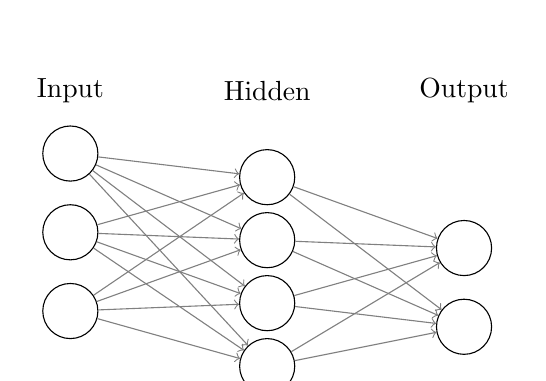
\begin{tikzpicture}[
    node distance=1.2cm,
    neuron/.style={circle, draw, minimum size=0.7cm, inner sep=0pt},
    every edge/.style={draw, ->, shorten >=1pt}
]
\foreach \i in {1,2,3}
  \node[neuron] (i\i) at (0,-\i) {};
\foreach \j in {1,2,3,4}
  \node[neuron] (h\j) at (2.5,-0.5-\j*0.8) {};
\foreach \k in {1,2}
  \node[neuron] (o\k) at (5,-1.2-\k*1.0) {};
\foreach \i in {1,2,3}
  \foreach \j in {1,2,3,4}
    \draw[->, gray] (i\i) -- (h\j);
\foreach \j in {1,2,3,4}
  \foreach \k in {1,2}
    \draw[->, gray] (h\j) -- (o\k);
\node at (0,-0.2) {Input};
\node at (2.5,-0.2) {Hidden};
\node at (5,-0.2) {Output};
\end{tikzpicture}
\caption{A fully connected feedforward network with three inputs, one hidden layer,
and two outputs.}
\label{fig:mlp}
\end{figure}

\section{Forward propagation and loss}

For a batch of examples, store activations as matrices with one example per row. The
forward pass is a sequence of affine transformations and activations. The training
objective is the average loss plus regularisation:
\begin{align}
    J = \frac{1}{n}\sum_{i=1}^n \ell(y_i,\hat{\mathbf{y}}_i)
    + \lambda\sum_{l}\norm{\mathbf{W}_l}_F^2.
\end{align}
For regression, use squared error; for binary classification, binary cross-entropy;
for multiclass, categorical cross-entropy. These choices are not arbitrary: they
correspond to Gaussian, Bernoulli, and categorical likelihoods respectively.

\section{Backpropagation}

Backpropagation is the chain rule applied efficiently to a computation graph. For a
single layer with pre-activation $\mathbf{z} = \mathbf{W}\mathbf{a}_{\mathrm{prev}}+
\mathbf{b}$ and activation $\mathbf{a}=\phi(\mathbf{z})$, define the error signal
$\boldsymbol{\delta} = \partial J/\partial \mathbf{z}$. Then
\begin{align}
    \frac{\partial J}{\partial \mathbf{W}}
    &= \boldsymbol{\delta}\,\mathbf{a}_{\mathrm{prev}}^\top, &
    \frac{\partial J}{\partial \mathbf{b}} &= \boldsymbol{\delta},\\
    \boldsymbol{\delta}_{\mathrm{prev}}
    &= \left(\mathbf{W}^\top\boldsymbol{\delta}\right)\odot
       \phi'(\mathbf{z}_{\mathrm{prev}}),
\end{align}
where $\odot$ is elementwise multiplication. Starting from the output layer, these
recursions propagate the error backward through the network. Automatic
differentiation libraries implement the same idea for arbitrary computation graphs.

\section{Training deep networks}

\begin{itemize}
    \item \textbf{Initialisation}: Xavier/Glorot initialisation for $\tanh$ and He
    initialisation for ReLU keep activations and gradients well scaled.
    \item \textbf{Normalisation}: batch normalisation or layer normalisation stabilises
    training and allows larger learning rates.
    \item \textbf{Regularisation}: weight decay, dropout, data augmentation, and early
    stopping reduce overfitting.
    \item \textbf{Optimisation}: Adam or SGD with momentum; learning-rate schedules
    matter.
    \item \textbf{Monitoring}: track training and validation loss, gradient norms, and
    activation statistics.
\end{itemize}

\section{Generalisation}

Deep networks have far more parameters than classical models, yet they generalise well
in many settings. Classical bias--variance intuition is incomplete: very large
networks can interpolate the training data and still perform well on test data, a
phenomenon sometimes called \emph{double descent}. Explanations include implicit
regularisation from SGD, architectural inductive biases, and the geometry of
overparameterised loss landscapes. The practical lesson is that capacity alone does
not determine generalisation; data, optimisation, and architecture interact.

\coderef{Code/neural_networks.py}

\chapter{Deep Learning}
\label{ch:deep}

Deep learning uses neural networks with many layers and architectures tailored to the
structure of the data.

\section{Convolutional neural networks}

A convolution layer applies a small learnable filter across spatial positions:
\begin{align}
    y_{i,j,k} = \sum_{a,b,c} W_{a,b,c,k}\,x_{i+a,j+b,c} + b_k.
\end{align}
Convolutions exploit locality and translation equivariance, and they share weights
across positions, which drastically reduces the parameter count compared with a fully
connected layer. A typical CNN alternates convolution, nonlinearity, and pooling
(or strided convolution), then uses a global pooling or fully connected head.
Landmark architectures include LeNet, AlexNet, VGG, GoogLeNet, and ResNet. Residual
connections $\mathbf{y}=\mathbf{x}+F(\mathbf{x})$ make very deep networks trainable.

\section{Sequence models}

Recurrent networks process a sequence one step at a time and maintain a hidden state:
\begin{align}
    \mathbf{h}_t = \phi(\mathbf{W}_h\mathbf{h}_{t-1}+\mathbf{W}_x\mathbf{x}_t+\mathbf{b}).
\end{align}
Backpropagation through time is the chain rule unrolled over the sequence. Long
dependencies suffer from vanishing or exploding gradients; gated architectures such as
LSTM and GRU use gates to control information flow. For many sequence tasks,
transformers have largely replaced recurrent models.

\section{Attention and transformers}

Scaled dot-product attention computes
\begin{align}
    \mathrm{Attention}(\mathbf{Q},\mathbf{K},\mathbf{V})
    = \mathrm{softmax}\!\left(\frac{\mathbf{Q}\mathbf{K}^\top}{\sqrt{d_k}}\right)\mathbf{V}.
\end{align}
Multi-head attention runs several attention operations in parallel and concatenates
the results. A transformer block combines multi-head attention with a position-wise
feedforward network, residual connections, and layer normalisation. Because attention
is permutation-equivariant, positional encodings are added to inject order.
Transformers underlie modern language models and have been adapted to vision, audio,
and scientific data.

\section{Generative models}

Generative models learn a distribution over data. Important families include:
\begin{itemize}
    \item \textbf{Autoencoders}: learn a bottleneck representation by reconstructing
    the input; denoising and variational autoencoders add noise or a probabilistic
    latent variable.
    \item \textbf{Variational autoencoders (VAEs)}: maximise the evidence lower bound
    (ELBO), balancing reconstruction against a KL penalty on the latent distribution.
    \item \textbf{Generative adversarial networks (GANs)}: train a generator and a
    discriminator in a minimax game.
    \item \textbf{Diffusion models}: learn to reverse a gradual noising process.
\end{itemize}

\section{Transfer learning and data efficiency}

Large models are often pretrained on a broad dataset and then fine-tuned on a small
target dataset. Fine-tuning can update all parameters or only a subset; linear probing
trains only a new head. Data augmentation, self-supervised pretraining, and
distillation are further tools for improving data efficiency. When applying deep
learning, start with a pretrained model if the domain is close to a standard one, and
only train from scratch when you have enough data and compute.

\coderef{Code/deep_learning.py}

\chapter{Probabilistic Models}
\label{ch:probmodels}

\section{Graphical models}

A Bayesian network represents a joint distribution as a directed acyclic graph:
\begin{align}
    p(\mathbf{x}) = \prod_{i=1}^d p\big(x_i \mid \mathrm{parents}(x_i)\big).
\end{align}
The graph encodes conditional independences, which can be read off with
d-separation. Graphical models provide a compact language for complex joint
distributions and a recipe for inference. Markov random fields use undirected graphs
and factor potentials instead of conditional probabilities.

\section{Mixture models and the EM algorithm}

A Gaussian mixture model assumes
\begin{align}
    p(\mathbf{x}) = \sum_{k=1}^K \pi_k\,\mathscr{N}(\mathbf{x}\mid
    \boldsymbol{\mu}_k,\boldsymbol{\Sigma}_k),
    \qquad \sum_k \pi_k = 1.
\end{align}
Latent variables $z_i \in \{1,\ldots,K\}$ indicate the component that generated each
observation. The log-likelihood is not concave because of the sum inside the log, so
we use expectation--maximisation (EM). The E-step computes responsibilities
\begin{align}
    \gamma_{ik} = \frac{\pi_k\,\mathscr{N}(\mathbf{x}^{(i)}\mid\boldsymbol{\mu}_k,
    \boldsymbol{\Sigma}_k)}{\sum_{j=1}^K \pi_j\,\mathscr{N}(\mathbf{x}^{(i)}\mid
    \boldsymbol{\mu}_j,\boldsymbol{\Sigma}_j)},
\end{align}
and the M-step updates the parameters using the responsibilities as soft assignments.
Each iteration increases the likelihood (or leaves it unchanged), but EM can converge
to a local maximum.

\section{Hidden Markov models}

An HMM models a sequence of observations $\mathbf{x}_1,\ldots,\mathbf{x}_T$ generated
by a latent Markov chain $z_1,\ldots,z_T$:
\begin{align}
    p(\mathbf{x}_{1:T},\mathbf{z}_{1:T})
    = p(z_1)\prod_{t=2}^T p(z_t\mid z_{t-1})
      \prod_{t=1}^T p(\mathbf{x}_t\mid z_t).
\end{align}
The forward--backward algorithm computes marginal posteriors in linear time; Viterbi
finds the most likely state sequence; Baum--Welch is EM for HMMs. HMMs remain useful
for speech, bioinformatics, and simple sequence labelling, although deep sequence
models are now more common for large datasets.

\section{Variational inference and MCMC}

For complex models the posterior $p(\mathbf{z}\mid\mathbf{x})$ is intractable.
\emph{Variational inference} chooses a tractable family $q_\phi(\mathbf{z})$ and
maximises the evidence lower bound
\begin{align}
    \mathcal{L}(\phi)
    = \E_{q_\phi(\mathbf{z})}\big[\log p(\mathbf{x},\mathbf{z})
      - \log q_\phi(\mathbf{z})\big]
    = \log p(\mathbf{x}) - D_{\mathrm{KL}}\big(q_\phi(\mathbf{z})\,\|\,
      p(\mathbf{z}\mid\mathbf{x})\big).
\end{align}
Maximising the ELBO is equivalent to minimising the KL divergence to the true
posterior. \emph{Markov chain Monte Carlo} (MCMC) instead draws samples from the
posterior; it is asymptotically exact but can be slow. Variational methods are faster
and scale better; MCMC is preferable when accuracy is critical and the model is
moderate-sized.

\coderef{Code/probabilistic_models.py}

\chapter{Reinforcement Learning}
\label{ch:rl}

\section{Markov decision processes}

A Markov decision process (MDP) is a tuple
$(\mathcal{S},\mathcal{A},P,R,\gamma)$: states, actions, transition probabilities
$P(s'\mid s,a)$, rewards $R(s,a)$, and a discount factor $\gamma \in [0,1)$. At each
step the agent observes state $s_t$, chooses action $a_t$, receives reward $r_t$, and
transitions to $s_{t+1}$. A policy $\pi(a\mid s)$ specifies the action distribution.

The \emph{return} is the discounted sum of rewards:
\begin{align}
    G_t = \sum_{k=0}^{\infty}\gamma^k r_{t+k}.
\end{align}
The \emph{state-value function} and \emph{action-value function} are
\begin{align}
    V^\pi(s) &= \E_\pi[G_t\mid s_t=s], &
    Q^\pi(s,a) &= \E_\pi[G_t\mid s_t=s,a_t=a].
\end{align}
The optimal policy maximises these values; at least one deterministic optimal policy
exists for finite MDPs.

\section{Bellman equations}

The Bellman expectation equations are
\begin{align}
    V^\pi(s) &= \sum_a \pi(a\mid s)\sum_{s'}P(s'\mid s,a)
      \big[R(s,a)+\gamma V^\pi(s')\big],\\
    Q^\pi(s,a) &= \sum_{s'}P(s'\mid s,a)
      \big[R(s,a)+\gamma\sum_{a'}\pi(a'\mid s')Q^\pi(s',a')\big].
\end{align}
The Bellman optimality equations replace the policy average with a max:
\begin{align}
    V^\star(s) = \max_a \sum_{s'}P(s'\mid s,a)
    \big[R(s,a)+\gamma V^\star(s')\big].
\end{align}
If the model is known, \emph{policy evaluation}, \emph{policy iteration}, and
\emph{value iteration} solve the MDP exactly (up to numerical precision). Value
iteration repeatedly applies the Bellman optimality operator; it converges because the
operator is a $\gamma$-contraction in the sup norm.

\section{Model-free learning}

When the transition model is unknown, the agent learns from experience.
\emph{Monte Carlo} methods average complete returns. \emph{Temporal-difference} (TD)
methods bootstrap from current value estimates. TD(0) updates
\begin{align}
    V(s_t) \leftarrow V(s_t) + \alpha\big[r_t+\gamma V(s_{t+1})-V(s_t)\big].
\end{align}
SARSA is on-policy TD control:
\begin{align}
    Q(s_t,a_t) \leftarrow Q(s_t,a_t)
    + \alpha\big[r_t+\gamma Q(s_{t+1},a_{t+1})-Q(s_t,a_t)\big].
\end{align}
Q-learning is off-policy:
\begin{align}
    Q(s_t,a_t) \leftarrow Q(s_t,a_t)
    + \alpha\big[r_t+\gamma\max_{a'}Q(s_{t+1},a')-Q(s_t,a_t)\big].
\end{align}
Q-learning converges to $Q^\star$ under suitable conditions on the learning rate and
exploration.

\section{Exploration versus exploitation}

An agent must balance trying actions that may be better (exploration) against using
what it already knows (exploitation). $\epsilon$-greedy chooses a random action with
probability $\epsilon$ and the greedy action otherwise. Softmax exploration, optimistic
initialisation, and upper-confidence bounds are alternatives. In large state spaces,
value functions are approximated by neural networks; deep Q-learning (DQN) stabilises
this with experience replay and target networks.

\section{Policy-gradient methods}

Policy-gradient methods optimise the policy directly. The REINFORCE estimator is
\begin{align}
    \nabla_\theta J(\theta)
    = \E_\pi\big[G_t\,\nabla_\theta\log\pi_\theta(a_t\mid s_t)\big].
\end{align}
It is unbiased but has high variance; subtracting a baseline $b(s_t)$ that does not
depend on the action reduces variance without introducing bias:
\begin{align}
    \nabla_\theta J(\theta)
    = \E_\pi\big[(G_t-b(s_t))\,
      \nabla_\theta\log\pi_\theta(a_t\mid s_t)\big].
\end{align}
Actor--critic methods learn both a policy (actor) and a value function (critic); the
critic supplies the baseline and the advantage estimate. Modern algorithms such as
A2C, PPO, and SAC build on these ideas.

\section{Practical considerations}

Reinforcement learning is notoriously sample-inefficient and sensitive to reward
design. Reward shaping can speed learning but may introduce unintended incentives.
Environments can be non-stationary, and policies trained in simulation may not
transfer to the real world. Evaluation requires multiple seeds and careful attention
to variance.

\coderef{Code/reinforcement_learning.py}

\chapter{Statistical Learning Theory}
\label{ch:slt}

\section{Empirical risk minimisation}

A learning algorithm chooses a hypothesis $h$ from a class $\mathcal{H}$ based on a
training sample $S=((\mathbf{x}^{(1)},y_1),\ldots,(\mathbf{x}^{(n)},y_n))$. The
empirical risk is
\begin{align}
    \hat{\risk}_S(h) = \frac{1}{n}\sum_{i=1}^n \ell(y_i,h(\mathbf{x}^{(i)})),
\end{align}
and ERM returns $\hat{h}=\arg\min_{h\in\mathcal{H}}\hat{\risk}_S(h)$. The central
question is how close $\risk(\hat{h})$ is to $\risk(h^\star)$, where
$h^\star=\arg\min_{h\in\mathcal{H}}\risk(h)$ is the best hypothesis in the class.

\section{Error decomposition}

The excess risk decomposes into \emph{approximation error} and \emph{estimation
error}:
\begin{align}
    \risk(\hat{h}) - \risk(h^\star_{\mathcal{H}})
    \leq \underbrace{\risk(h^\star_{\mathcal{H}}) -
      \inf_{h}\risk(h)}_{\text{approximation}}
    + \underbrace{\risk(\hat{h}) - \risk(h^\star_{\mathcal{H}})}_{\text{estimation}}.
\end{align}
A richer class reduces approximation error but increases estimation error. This is
the learning-theoretic version of the bias--variance trade-off. Regularisation
restricts the effective complexity of the class.

\section{PAC learning}

Probably approximately correct (PAC) learning asks for a hypothesis whose risk is
within $\epsilon$ of the best in the class with probability at least $1-\delta$. For a
finite hypothesis class, the union bound gives: if
\begin{align}
    n \geq \frac{1}{2\epsilon^2}
    \log\frac{2|\mathcal{H}|}{\delta},
\end{align}
then with probability at least $1-\delta$, every $h\in\mathcal{H}$ satisfies
$|\risk(h)-\hat{\risk}_S(h)| \leq \epsilon$. The sample complexity grows only
logarithmically with the number of hypotheses. This bound is loose but illustrates why
finite, simple model classes are easy to learn.

\section{VC dimension}

For binary classification, the VC dimension of $\mathcal{H}$ is the size of the
largest set that $\mathcal{H}$ can \emph{shatter} (label in all possible ways). In
$d$ dimensions, linear classifiers have VC dimension $d+1$; the class of all
axis-aligned rectangles in $\R^2$ have VC dimension $4$ (and $2d$ in $\R^d$); a one-nearest-neighbour classifier can
shatter any finite set but has infinite VC dimension. Infinite VC dimension does not
imply failure, but it means that uniform convergence guarantees cannot be obtained
from VC theory alone.

The fundamental theorem of statistical learning (for binary classification) states
that a hypothesis class is PAC-learnable if and only if it has finite VC dimension.
Generalisation bounds are typically of the form
\begin{align}
    \risk(h) \leq \hat{\risk}_S(h)
    + O\!\left(\sqrt{\frac{\mathrm{VC}(\mathcal{H})}{n}}\right)
\end{align}
with logarithmic confidence terms. These bounds are worst-case and often pessimistic
for modern overparameterised models.

\section{Rademacher complexity and margin theory}

Rademacher complexity measures how well a hypothesis class can fit random noise:
\begin{align}
    \mathfrak{R}_n(\mathcal{H})
    = \E_{S,\boldsymbol{\sigma}}\left[
      \sup_{h\in\mathcal{H}}\frac{1}{n}\sum_{i=1}^n \sigma_i h(\mathbf{x}^{(i)})
    \right],
\end{align}
where $\sigma_i \in \{-1,+1\}$ are independent Rademacher variables. It yields
data-dependent generalisation bounds. Margin-based analysis explains why large-margin
classifiers can generalise even when their VC dimension is large: what matters is the
margin distribution, not just the raw parameter count.

\section{Double descent and modern practice}

Classical theory predicts that models with more parameters than data should overfit
badly. In practice, deep networks and other overparameterised models can interpolate
the training data and still generalise. Test error often follows a \emph{double
descent} curve: it decreases, peaks near the interpolation threshold, and then
decreases again as capacity grows. This has motivated research on implicit
regularisation, benign overfitting, and the geometry of overparameterised models.

The practical implications are:
\begin{itemize}
    \item Do not choose model size solely from classical parameter-counting bounds.
    \item Use validation data and learning curves rather than theoretical bounds alone.
    \item Regularisation, data augmentation, and early stopping remain effective.
    \item Theory is most useful for understanding \emph{why} and \emph{when} methods
    work, not for predicting benchmark accuracy.
\end{itemize}

\coderef{Code/learning_theory.py}

\chapter{Tools}
\label{ch:tools}

The Python ecosystem is the default for applied machine learning. The table below summarises the main libraries used in these notes.

\begin{center}
\renewcommand{\arraystretch}{1.25}
\begin{tabularx}{\textwidth}{@{}l>{\raggedright\arraybackslash}X@{}}
\toprule
Library & Role \\
\midrule
\texttt{NumPy} & $N$-dimensional arrays, linear algebra, random numbers. \\
\texttt{pandas} & Tabular data manipulation, cleaning, and exploratory analysis. \\
\texttt{matplotlib} & Plotting and visualisation. \\
\texttt{scikit-learn} & Classical ML: regression, classification, clustering, model selection,
preprocessing, pipelines, metrics. \\
\texttt{XGBoost} & Gradient-boosted trees with regularisation and efficient split finding. \\
\texttt{PyTorch} & Deep learning with dynamic computation graphs and automatic differentiation. \\
\texttt{TensorFlow} & Deep learning with a high-level API and production deployment tools. probably the most popular framework
nowadays for building, training, and querying machine
learning models. \\
\texttt{Keras} & a very popular library for neural networks
and regression models that easily integrates on top of
TensorFlow \\ 
\texttt{JAX} & Composable numerical computing and automatic differentiation. \\
\texttt{seaborn} & Statistical data visualization. \\
\bottomrule
\end{tabularx}
\end{center}

\section{Installing the companion code}

The minimal environment for the companion scripts is
\begin{pycode}
python -m venv .venv
source .venv/bin/activate        # Windows: .venv\Scripts\activate
pip install -r Code/requirements.txt
\end{pycode}
The deep-learning script additionally requires PyTorch:
\begin{pycode}
pip install torch torchvision
\end{pycode}

\section{Reproducibility checklist}

\begin{enumerate}
    \item Fix random seeds for data splitting, initialisation, and stochastic
    optimisation.
    \item Record library versions and hardware.
    \item Separate training, validation, and test data; never tune on the test set.
    \item Report mean and standard deviation over multiple runs when results are
    stochastic.
    \item Save the exact command, configuration, and data version used to produce each
    result.
\end{enumerate}

\section{A minimal workflow}

A reliable baseline workflow is:
\begin{enumerate}
    \item Load and inspect the data; check missing values, class balance, and leakage.
    \item Split into training and test sets before any preprocessing.
    \item Build a simple baseline (mean predictor, logistic regression, or a small
    tree).
    \item Put preprocessing and the model in a pipeline.
    \item Tune a small number of hyperparameters with cross-validation.
    \item Evaluate once on the test set; inspect errors and calibration.
    \item Only then move to more complex models or deep learning.
\end{enumerate}

\chapter{Resources}
\label{ch:resources}

\section{People}

\href{https://www.cs.toronto.edu/~rgrosse/}{Roger Grosse}, \href{https://www.cs.toronto.edu/~murat/}{Murat Erdogdu}, \href{https://www.cs.toronto.edu/~zemel/}{Richard Zemel}, \href{https://www.cs.toronto.edu/~juan/}{Juan Felipe Carrasquilla}, \href{https://www.cs.toronto.edu/~emad/}{Emad Andrews}, \href{https://www.cs.toronto.edu/~amir/}{Amir-massoud Farahmand}.

\section{Courses}

\begin{enumerate}
    \item \href{https://web.stanford.edu/class/cme250/}{Stanford University --- CME 250:
    Introduction to Machine Learning}.
    \item \href{https://www.cs.toronto.edu/~rgrosse/courses/csc321_2018/}{University of
    Toronto --- CSC 321: Intro to Neural Networks and Machine Learning}.
    \item \href{https://www.d2l.ai/}{Dive into Deep Learning} --- an interactive,
    open-access deep-learning book.
\end{enumerate}

\section{Books}

\begin{enumerate}
    \item \emph{An Introduction to Statistical Learning with Applications in R}\cite{james2021introduction}. Accessible first text; strong on regression, classification, resampling, and trees. It has a dedicated URL \url{https://www.statlearning.com/}.
    \item \emph{The Elements of Statistical Learning}
    \cite{hastie2009elements}. The more theoretical companion to the previous book. See \url{https://hastie.su.domains/ElemStatLearn/}.
    \item \emph{Pattern Recognition}
    \cite{theodoridis2006pattern}. Broad coverage with a probabilistic emphasis.
    \item \emph{Information Theory, Inference, and Learning Algorithms}
    \cite{mackay2003information}. Beautiful treatment of inference and learning.
    \item \emph{Bayesian Reasoning and Machine Learning}
    \cite{barber2012bayesian}. Graphical models and Bayesian methods.
    \item \emph{Reinforcement Learning: An Introduction}
    \cite{sutton1998reinforcement}. The standard reference for RL.
    \item \emph{Mathematics for Machine Learning}
    \cite{deisenroth2020mathematics}. Linear algebra, calculus, and probability for ML.
    \item \emph{Understanding Machine Learning: From Theory to Algorithms}
    \cite{shalev2014understanding}. Learning theory and algorithmic foundations.
    \item \emph{Machine Learning: A Probabilistic Perspective}
    \cite{murphy2012machine}. Comprehensive probabilistic treatment.
    \item Mathematics for Machine Learning by Marc Peter Deisenroth, A.Aldo Faisal and Cheng Soon Ong
\end{enumerate}

\section{Online resources}

\begin{enumerate}
    \item \href{https://huggingface.co/}{Hugging Face}:
    \item \href{https://alexsemendinger.github.io/transformers-gentle-introduction}{Transformers: A Gentle Introduction}.
    \item \href{https://www.turing.ac.uk/about-us}{The Alan Turing Institute}.
\end{enumerate}

\section{Conferences}

\begin{enumerate}
    \item \href{https://womeninaisafety.toronto.acm.org/}{Women in AI Safety}.
    \item  NeurIPS, ICML, ICLR, UAI.
    \item 
\end{enumerate}

\section{Technologies}

\begin{enumerate}
    \item \href{https://numpy.org/doc/}{NumPy}.
    \item \href{https://scikit-learn.org/stable/user_guide.html}{scikit-learn user guide}.
    \item \href{https://pytorch.org/tutorials/}{PyTorch tutorials}.
    \item \href{https://www.tensorflow.org/tutorials}{TensorFlow tutorials}.
    \item \href{https://xgboost.readthedocs.io/}{XGBoost documentation}.
    \item \href{https://github.com/crewAIInc/crewAI}{CrewAI}.
    \item \href{https://github.com/OpenHands/OpenHands}{OpenHands}.
    \item \href{https://octo.axiomatic-ai.com/search}{Octo}.
    \item \href{https://marimo.io/}{marimo}.
\end{enumerate}

\section{Helpful websites}

\begin{enumerate}
    \item \href{https://stats.stackexchange.com/}{Cross Validated} --- a question and answer site for people interested in statistics.
    \item \href{https://www.kaggle.com/}{Kaggle} --- a platform for data science competitions and datasets.
    \item \href{https://arxiv.org/}{arXiv} --- a repository of electronic preprints of scientific papers in the fields of physics, mathematics, computer science, and quantitative biology.
\end{enumerate}

\backmatter
\printindex
\printbibliography

\end{document}
